% --------------------------------------------------------------------------------
% Concepts: Modules
% --------------------------------------------------------------------------------

% ================================================================================
\chapter{Modules}
% ================================================================================

% --------------------------------------------------------------------------------
\section{Introduction}
% --------------------------------------------------------------------------------

This chapter describes the modules in the toolbox. A \emph{module}
represents a well-defined process leading to images and (possibly)
an inference. \emph{Well-defined} here means that it corresponds
to a relevant musical perceptual phenomenon. Figure
\ref{Fig:ImageTransformationModules} gives an overview of what we
have in mind as a global picture.

\begin{figure}[h]
    \centering
    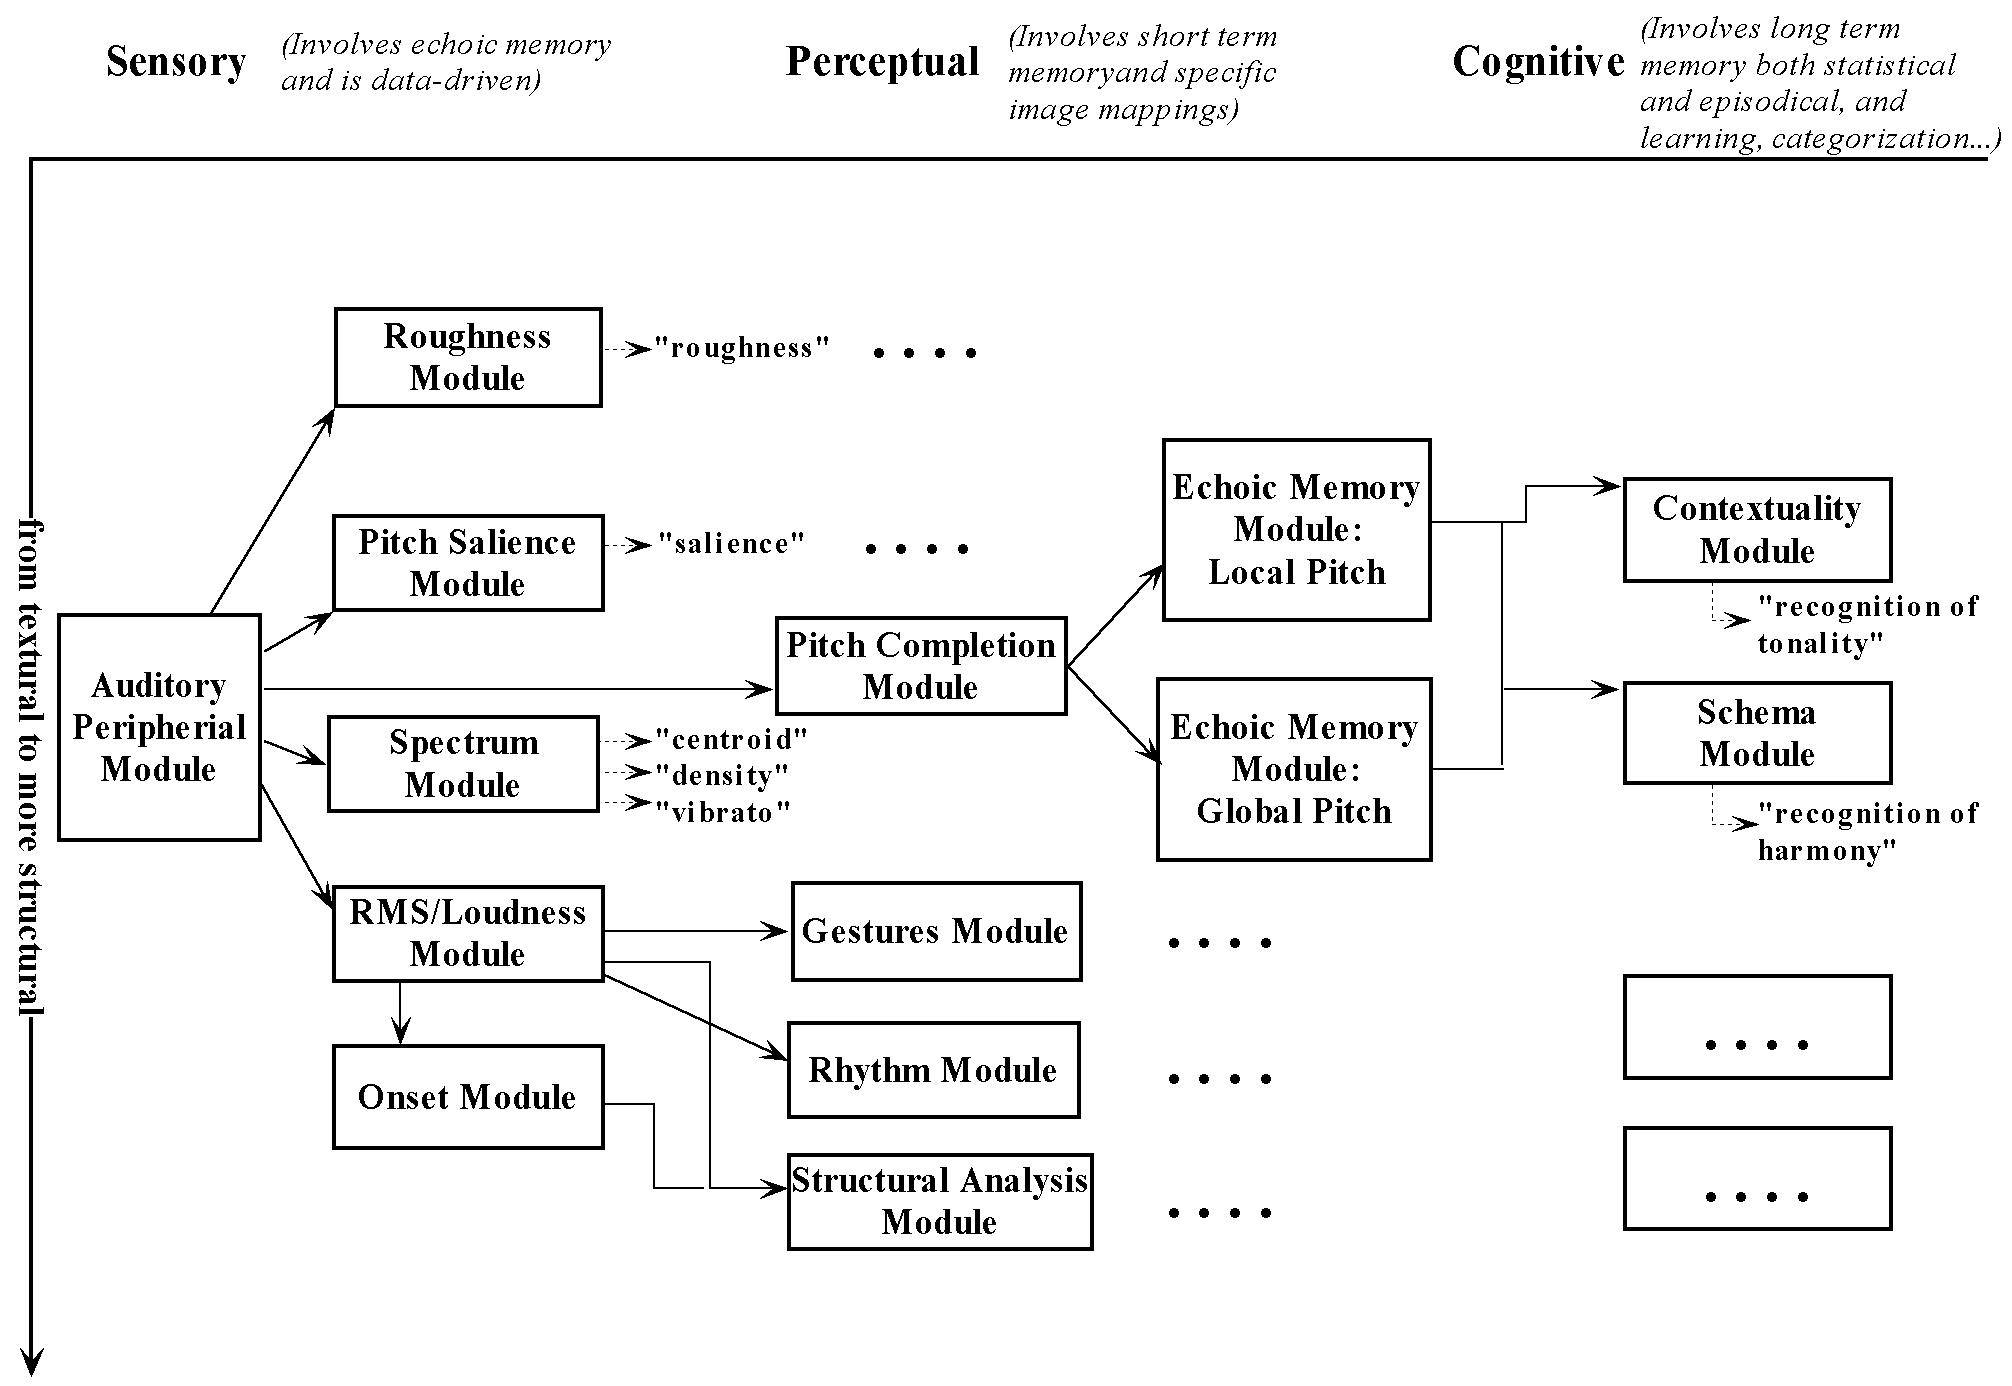
\includegraphics[width=\textwidth]{Graphics/ImageTransformationModules}
    \caption{Chart of image transformation modules, organized
    according to the distinction between sensory, perceptual, and
    cognitive information processing (horizontal axis), and from
    textural to structural (vertical axis). The chart is not
    exhaustive.}
    \label{Fig:ImageTransformationModules}
\end{figure}

The modules on the left are sensory based, the ones on the right
are cognition based and the ones in the middle are perception
based.
\begin{itemize}
    \item Sensory modules involve immediate memory and are based
    on stimulus-driven processing. We assume that they are located
    in the periphery of the auditory system.
    \item Perception modules involve short-term memory and
    specific image mapping from the temporal domain into the
    spatial domain. We assume that they are located in the brain
    stem.
    \item Cognitive modules involve long-term memory, learning and
    categorization. We assume that they are located in the cortex.
\end{itemize}
The modules are furthermore organized from texture (top) to
structure (bottom). This is obviously a simplification but one
that according to our feeling makes sense, at least to some
extent. You should be aware of the fact that this is just one
possible way to visualize the modules and that other
visualizations of the global picture are possible. Notice one more
feature of this chart, in particular the expressions between
quotes, such as "roughness". These labels refer to inferences
associated with the modules. In figure
\ref{Fig:ModulesHighlighted} the modules in the toolbox are
highlighted.

\begin{figure}[h]
    \centering
    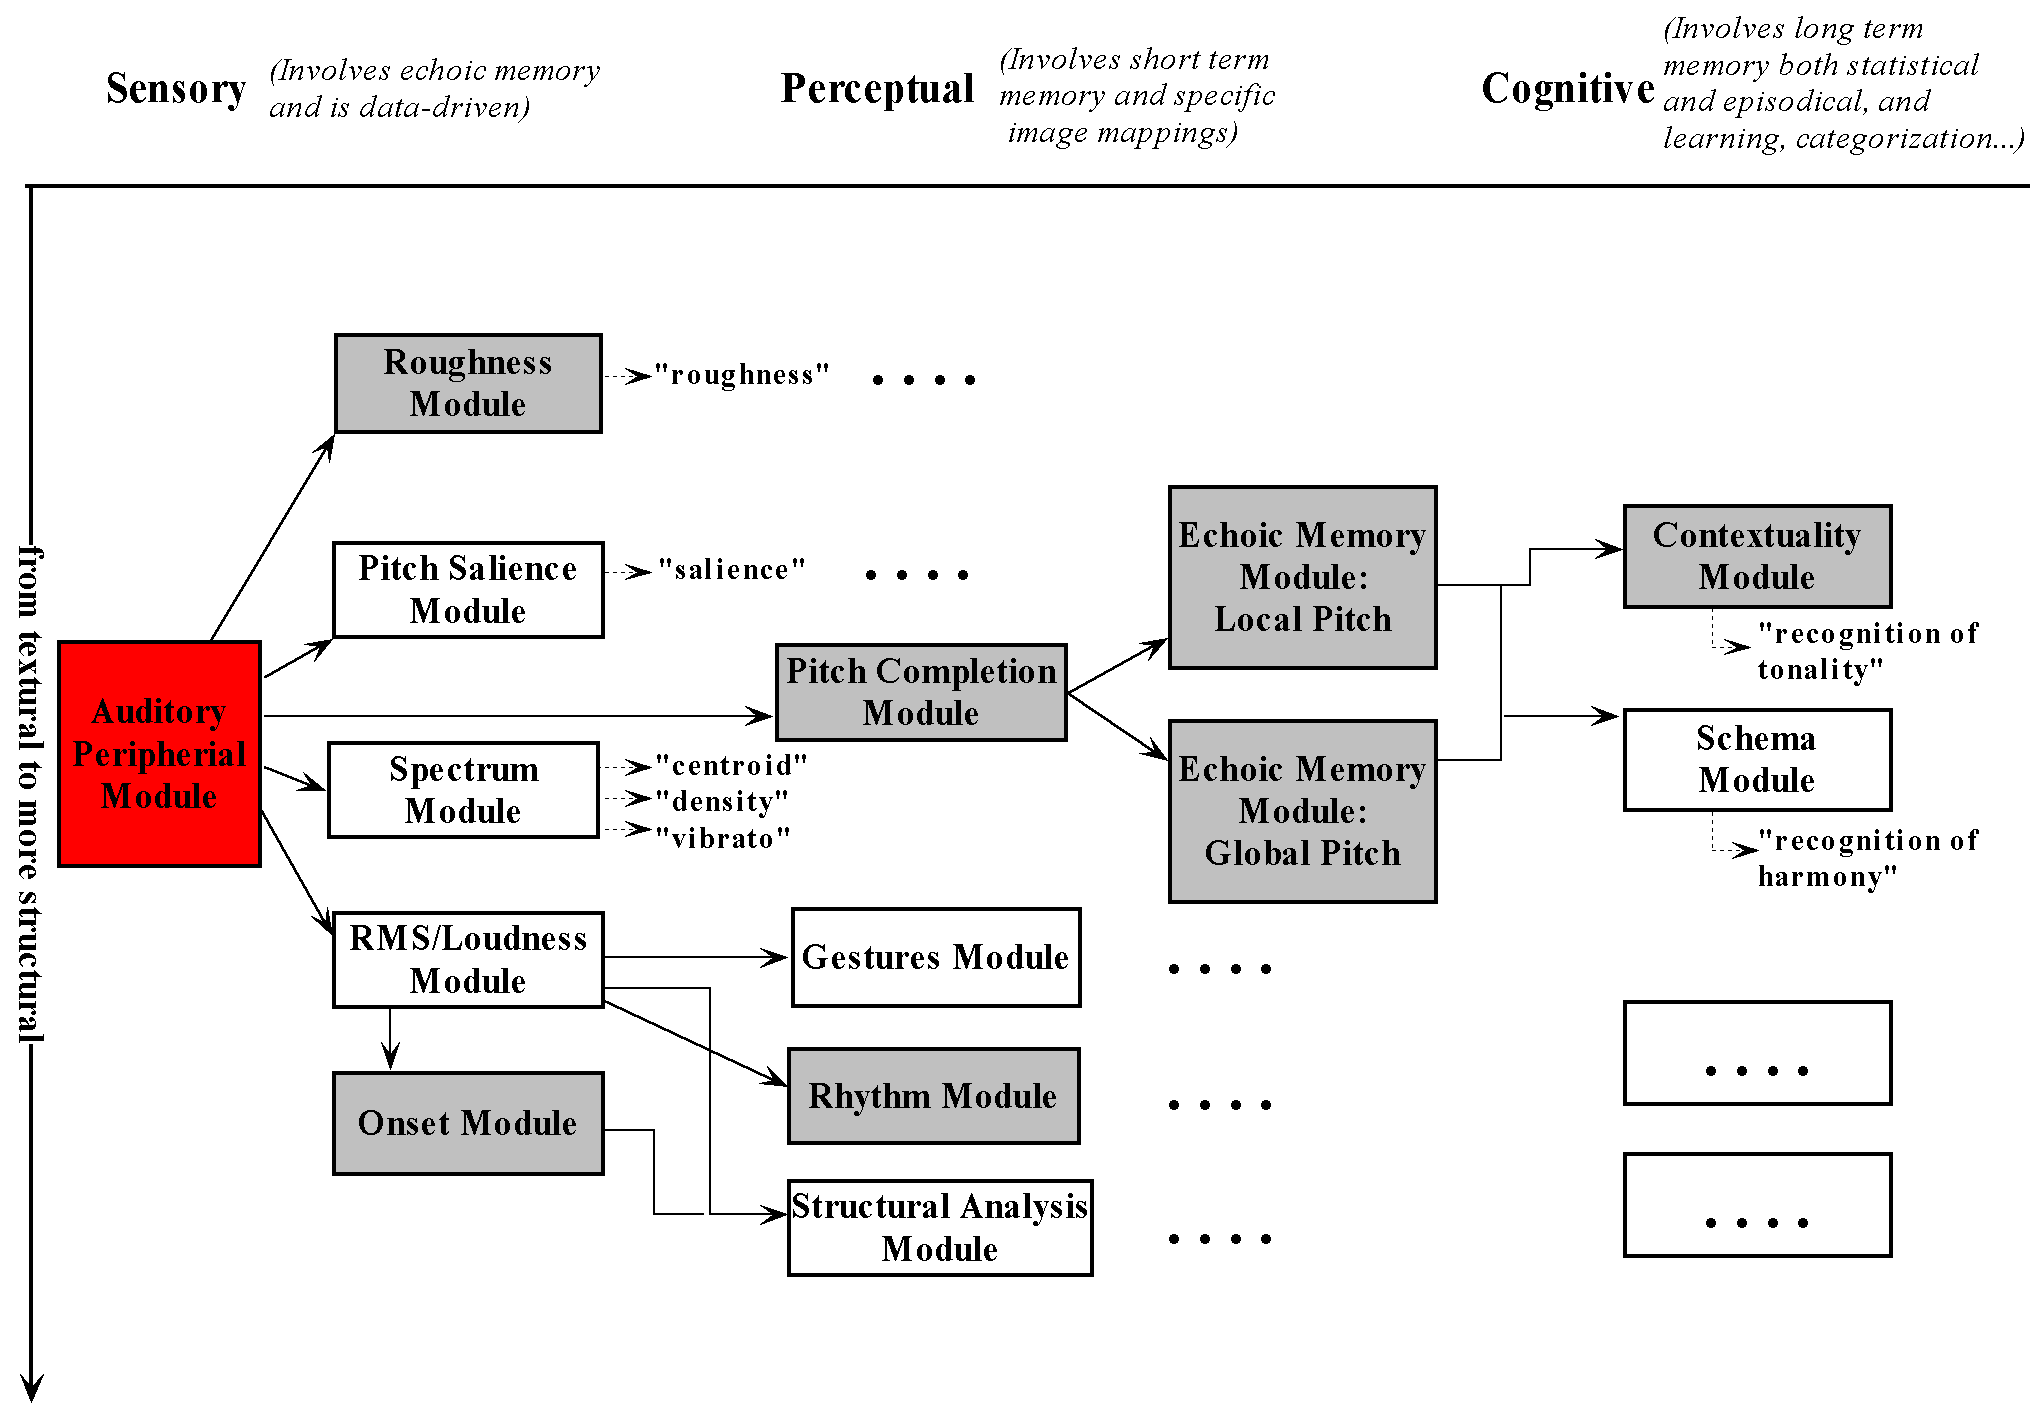
\includegraphics[width=\textwidth]{Graphics/ModulesHighlighted}
    \caption{Situation of the toolbox modules in the global conception}
    \label{Fig:ModulesHighlighted}
\end{figure}

Recall that a module is a well-defined process but that it may
consist of one or more toolbox functions. We learn you how to use
these functions while exploring the modules. If it is the first
time that you read this introduction you can skip the
functional-logical and signal processing descriptions and limit
yourself to the introductory description and the examples. This
should provide enough information to acquire an idea of what the
module is doing.

% --------------------------------------------------------------------------------
% --------------------------------------------------------------------------------
\newpage
\section{Auditory Peripheral Module}
% --------------------------------------------------------------------------------

% Make general target
\hypertarget{Concepts:AuditoryPeripheralModule}{}

% Make target for following functions:
\hypertarget{Concepts:IPEMCalcANI}{}
\hypertarget{Concepts:IPEMCalcANIFromFile}{}
\hypertarget{Concepts:IPEMLoadANI}{}
\hypertarget{Concepts:IPEMSaveANI}{}

\subsection{Introductory description}
% --------------------------------------------------------------------------------

The Auditory Peripheral Module (APM) (fig. \ref{Fig:ModulesAPM})
takes as input a sound and gives as output the \emph{auditory
primary image} which is a kind of physiological justified
representation of the auditory information stream along the VIIIth
cranial nerve. The musical signal is decomposed in different
subbands and represented as neural patterns. The patterns are
rate-codes, which means that they provide the probability of
neuronal firing during a short interval of time.
\begin{figure}[h]
    \centering
    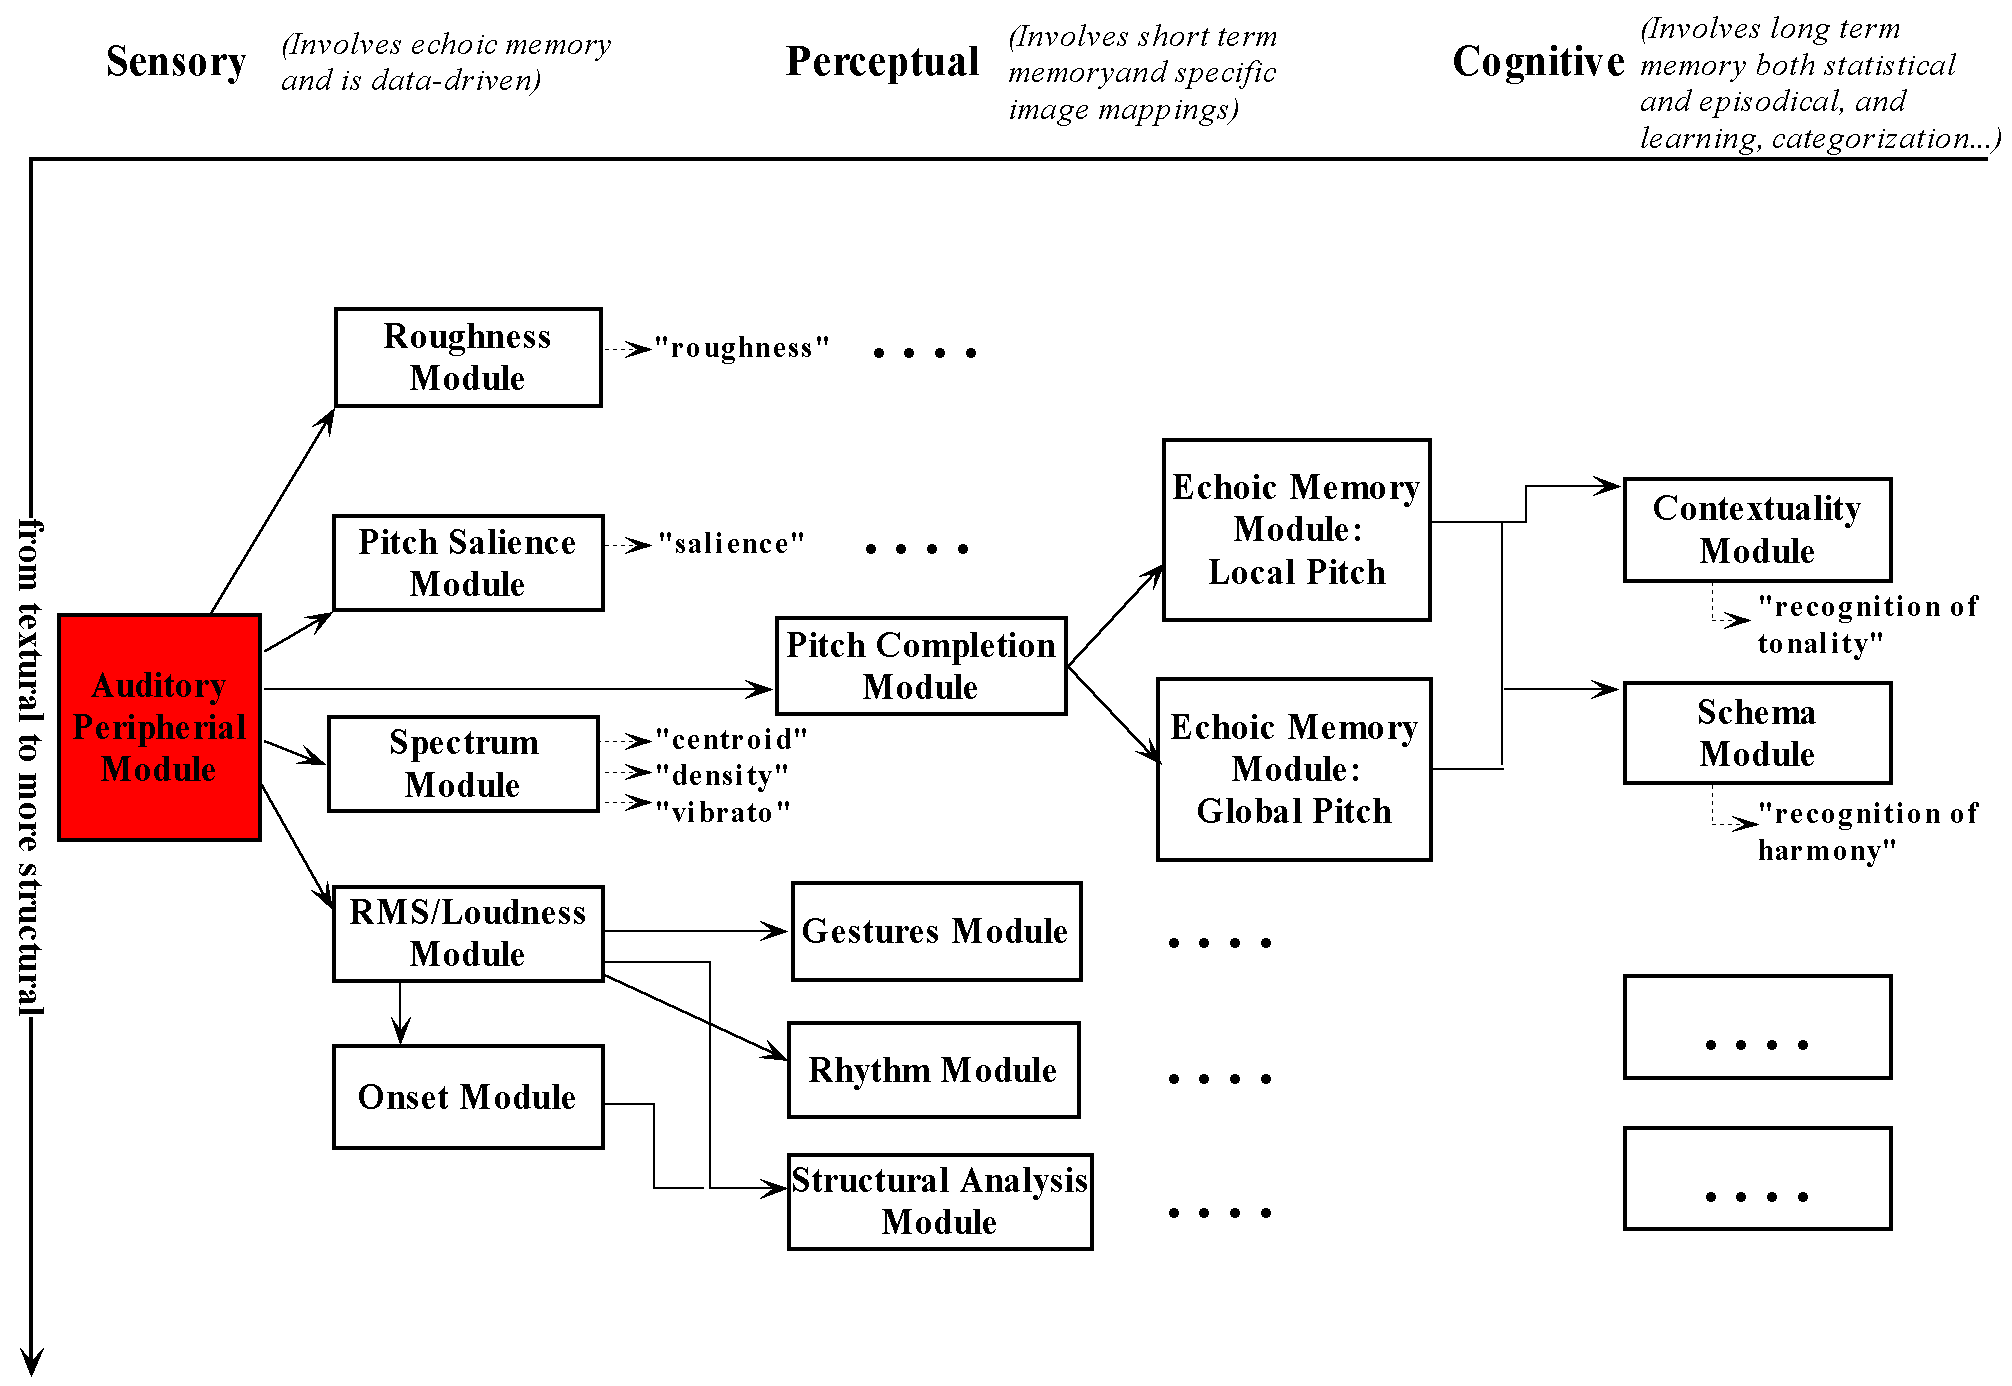
\includegraphics[width=\textwidth]{Graphics/ModulesAPM}
    \caption{Chart of image transformation modules, with APM highlighted}
    \label{Fig:ModulesAPM}
\end{figure}

The Auditory Peripheral Module that we use is an adapted version
of \citeA{VanImmerseelMartens:92} model of the auditory periphery.
The processing stages involve:
\begin{itemize}
\item
    Simulation of the filtering of the outer and middle ear.
\item
    Simulation of basilar membrane resonance in the inner ear. This is
    implemented by an array of band-pass filters whose center
    frequencies are spaced on a critical band scale (Bark scale).
    The bandwidth of each filter equals
    a critical band.
\item
    Simulation of a hair cell model. This converts the band-pass filtered signals into
    neural {\sl rate-code} patterns. This operation deals with half-wave rectification and
    dynamic range compression.
\end{itemize}

Figure \ref{Fig:APMModule} gives a view of the transformation of
sound into primary images.
\begin{figure}[h]
    \centering
    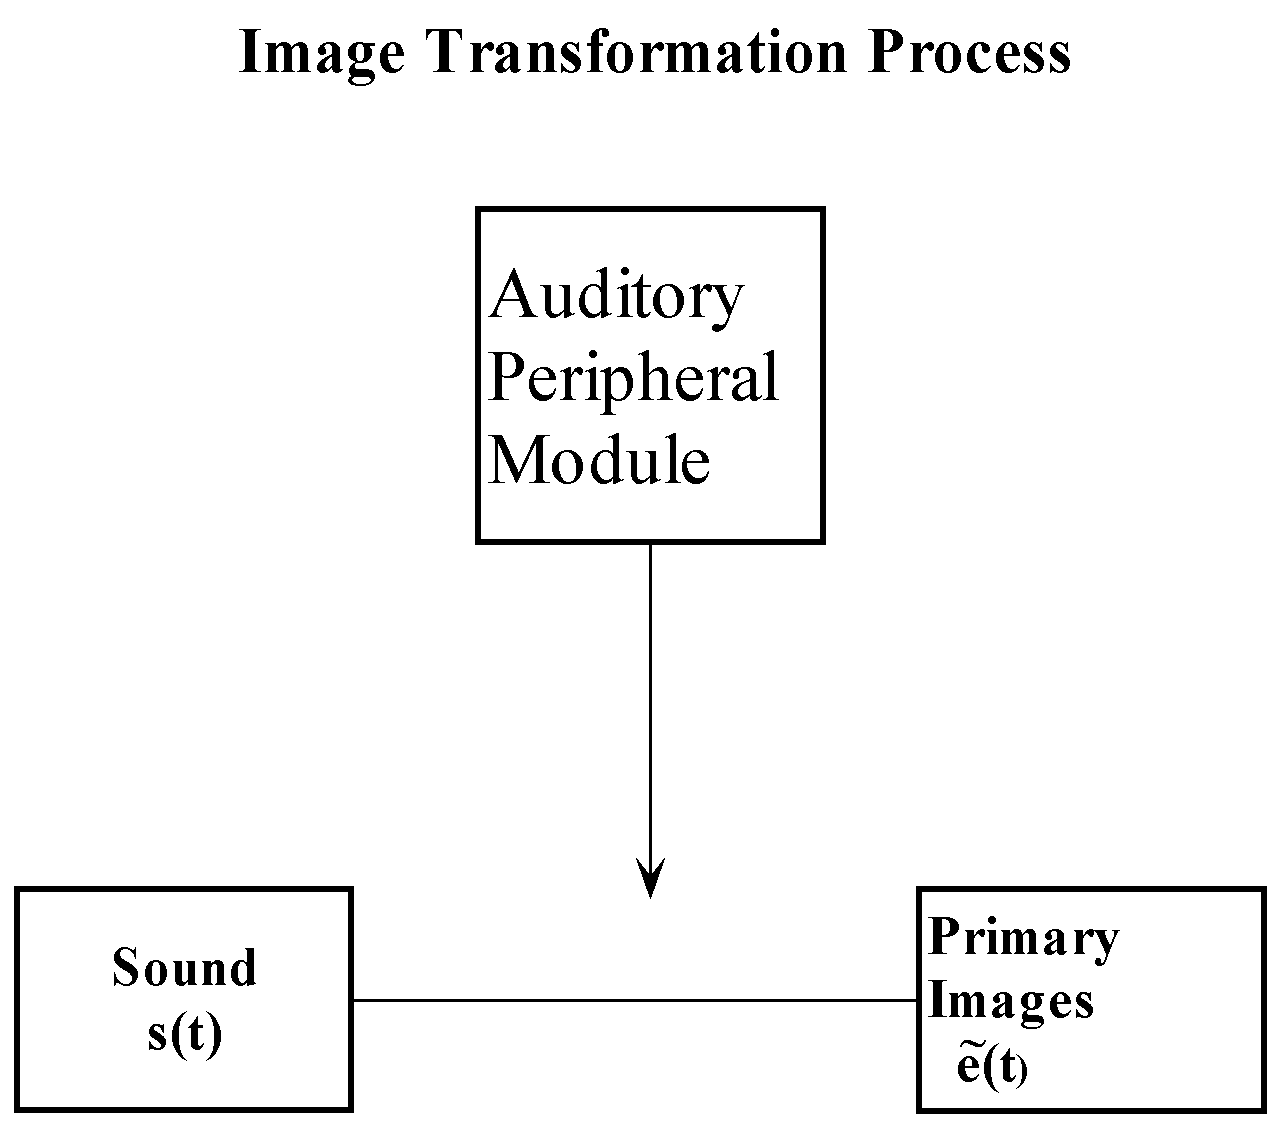
\includegraphics[width=\IPEMDefaultFigureWidth]{Graphics/APMModule}
    \caption{Image Transformation Process: Auditory Peripheral  Module}
    \label{Fig:APMModule}
\end{figure}

\subsection{Functional-logical description}
% --------------------------------------------------------------------------------

The APM can be described as a function which transforms a musical
sound signal $s(t)$ into a set of patterns $e_n(t)$ (with $n = 1,
2, ..., C$) that encode the responses of auditory neuronal fibers
spread along the basilar membrane (see Equation \ref{Eq1}). The
auditory filters, sometimes also called {\sl channels}, simulate
the neuronal band-pass characteristics and the firing rate
encoding. The frequency range covered by the auditory filters
depends on the center frequencies of the filters, the number of
chosen channels and the chosen distance between the channels. In
most of our simulations we chose forty channels ($C=40$), half a
critical band apart from each other. This covers a range from 140
Hz to 8877 Hz. As a short-hand we use the notation:

\begin{displaymath}
APM:~s(t) \rightarrow \left[
\begin{array}{l}
e_1(t) \\ e_2(t) \\ \cdots \\ e_{C}(t)
\end{array}
\right]=~e(t,c)~=~\tilde{e}(t)
\end{displaymath}
or, alternatively,
\begin{equation}
APM:~s(t) \rightarrow \tilde{e}(t) \label{Eq1}
\end{equation}

The pattern denoted $\tilde{e}(t)$ is called the \emph{primary
image} or \emph{auditory nerve image (ANI)} of $s(t)$. It should
be considered the auditory counterpart of D.~Marr's {\sl primal
sketch} in the domain of visual perception \cite{Marr:82}. The
tilde character here denotes a vector in which each
vector-component corresponds to one auditory filter. The arrow
represents a causal transformation, in this case from a sound into
the auditory nerve image.

In our terminology, a \emph{running vector} means that the values
of the vector-components change over time, where $t$ denotes time.
The pattern $\tilde{e}(t)$ thus represents the neural activation
in all subbands over subsequent time steps. The notation $e(t,c)$
means the same, whereas $e(t,c)$ for fixed $c$ is the neural
activation in one particular channel $c$.

\subsection{Signal processing description}
% --------------------------------------------------------------------------------
For a full description of this module we refer to
\citeA{VanImmerseelMartens:92}. We limit ourselves to a more technical
verbal summary.

The auditory peripheral module simulates the cochlear mechanical
filtering using an array of overlapping band-pass filters.
%The
%module provides rate-code patterns of neural discharge at the
%level of the auditory nerve, representing the amount of neural
%excitation during short time intervals.
The basic steps of this model, shown in figure
\ref{Fig:AuditoryModel} can be summarized as follows.

\begin{figure}[h]
    \centering
    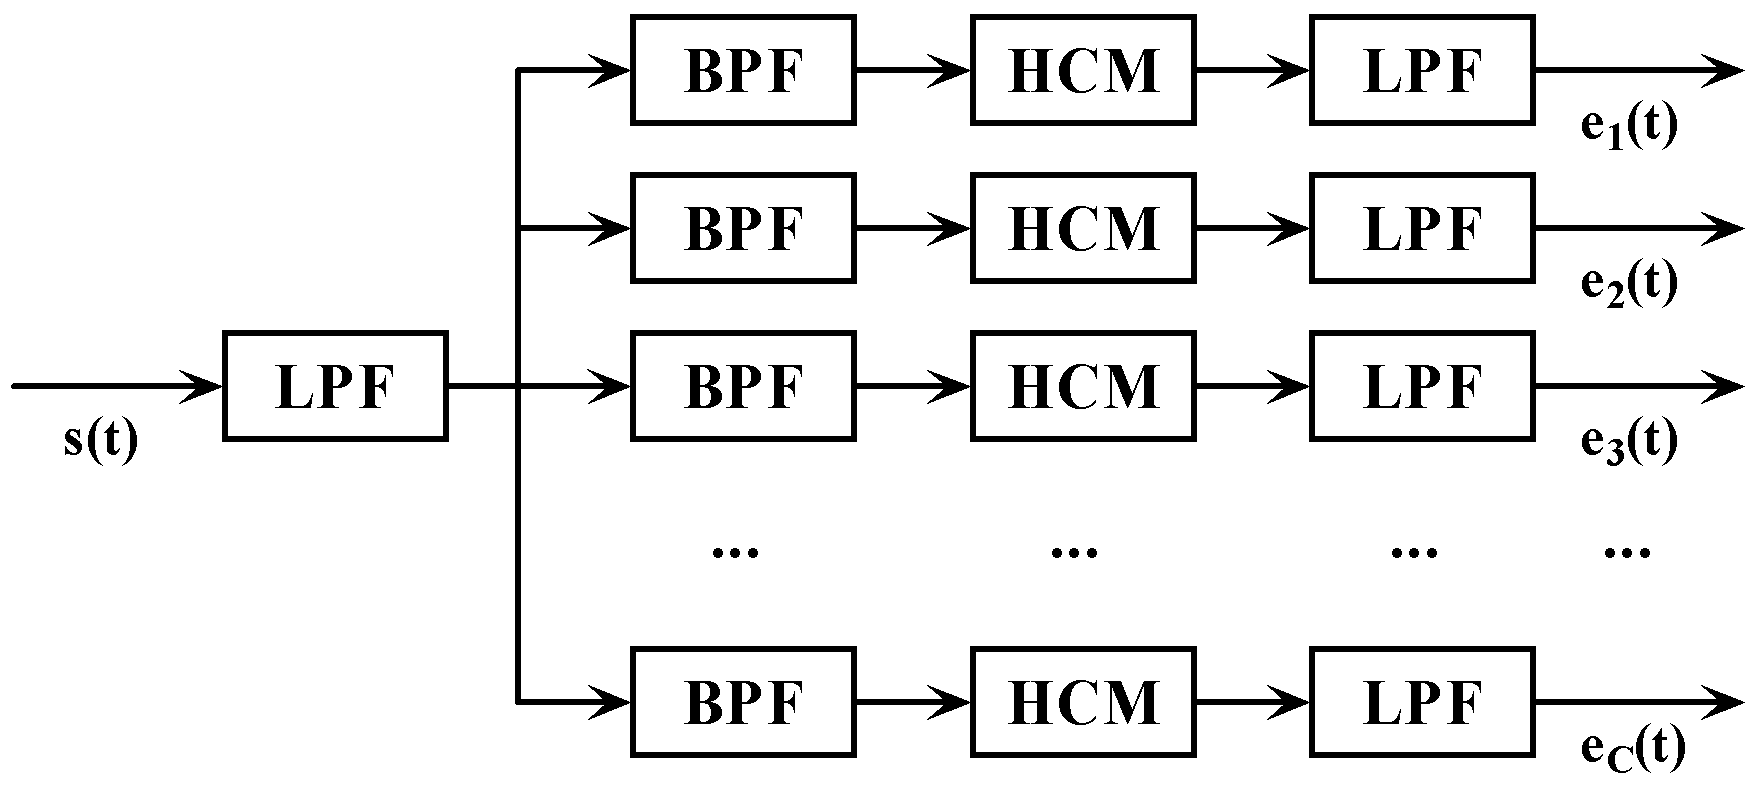
\includegraphics[width=\IPEMDefaultFigureWidth]{Graphics/AuditoryModel}
    \caption{Schema of the Auditory Peripheral Module. }
    \label{Fig:AuditoryModel}
\end{figure}

\begin{itemize}
\item
    The outer and inner ear filtering is implemented as a
    second-order low-pass filter (LPF) with a resonance frequency of
    4 kHz. This accounts for the overall frequency response of the
    ear, a coarse approximation to the Fletcher-Munson curves.
\item
    The filtering in the cochlea is implemented by an array of
    band-pass filters (BPF). In many of the simulations in this book,
    we use center frequencies that are spaced equidistantly on a
    critical band scale, having an overlap of half a critical band.
    Forty channels are used with center frequencies ranging from 141
    to 8877 Hz. The filters have a 3 dB bandwidth of one critical
    band; a low-frequency slope of about 10 dB per critical band unit
    and a high-frequency slope of about 20 dB per critical band unit.
\item
    The mechanical to neural transduction is performed by a hair cell
    model (HCM), which is assumed identical in all channels. The HCM
    is a forward-driven gain controlled amplifier that incorporates
    half-wave rectification and dynamic range compression. The HCM
    introduces distortion products that reinforce the low frequencies
    that correspond to the frequency of the beats.
\item
    A low-pass filter at 1250 Hz does an envelope extraction of the
    patterns in each channel. This low-pass filter accommodates for
    the loss of synchronization observed in the primary auditory
    nerve. The filter can be argued to have an effect on the width of
    the critical band for high $f_c$ although these may fall out of
    the scope of most musically relevant tones
    \cite{GreenwoodJoris:1996}.
\end{itemize}

The output $e(t,c)$ for fixed $c$ represents the rate-code of
neural discharge in channel $c$. This pattern is also called the
\emph{auditory nerve pattern} in channel $c$.

\subsection{Implementation}
% --------------------------------------------------------------------------------

\begin{tabularx}{\linewidth}{llX}
\hyperlink{FuncRef:IPEMCalcANI}{IPEMCalcANI} & - & Calculates auditory nerve image from signal\\
\hyperlink{FuncRef:IPEMCalcANIFromFile}{IPEMCalcANIFromFile} & - & Calculates auditory nerve image directly from sound file\\
\hyperlink{FuncRef:IPEMLoadANI}{IPEMLoadANI} & - & Loads auditory nerve image from .mat file\\
\hyperlink{FuncRef:IPEMSaveANI}{IPEMSaveANI} & - & Saves auditory nerve image to .mat file\\
\end{tabularx}

\subsection{Examples}
% --------------------------------------------------------------------------------

In this section we provide some examples of how to transform
musical signals into primary images (auditory nerve images). A
straightforward function is
\hyperlink{FuncRef:IPEMCalcANIFromFile}{IPEMCalcANIFromFile} which
allows you to read in a wav-file. If the wav-file
\emph{SchumannKurioseGeschichte.wav} is stored in the "Sounds"
subdirectory of the default input directory (see also the
\hyperlink{ReferenceManual:Installation}{installation}
instructions), and you agree with the default 40 subbands and the
overlap of 1/2 critical band, then the function is simply:\\

\IPEMCodeExtract{IPEMCalcANIFromFile('SchumannKurioseGeschichte.wav',[],[],1);}\\

Similarly, if \emph{ShepardCChord.wav} is stored in that same directory, you can write:\\

\IPEMCodeExtract{IPEMCalcANIFromFile('ShepardCChord.wav');}\\

The results should be similar to what you see on these pages
(except the score, of course):
\begin{enumerate}
\item
    Figure \ref{Fig:SchumannScore} shows the score of the
    \IPEMSound{Sounds/SchumannKurioseGeschichte.wav}{used
    excerpt of Schumann's Kuriose Geschichte}.
    \footnote{Robert Schumann "Kinderszenen-Kreisleriana", played
    by Martha Argerich (Deutsche Grammophon 410 653-2, 1984)}
\item
    Figure \ref{Fig:SchumannANIandAudioSignal} shows the results of processing
    this short excerpt with the Auditory Peripheral Module. The upper panel shows
    the waveform, the lower panel shows the primary image.
\item
    Figure \ref{Fig:ShepardCChordANIandAudioSignal} shows the results of processing
    \IPEMSound{Sounds/ShepardCChord.wav}{a signal consisting of
    the C major chord, build up from 3 Shepard tones} with the Auditory Peripheral Module.
    Again, the upper panel shows the waveform, the lower panel shows the primary image.
\end{enumerate}

To generate a Shepard-chord yourself, you can type (see
\hyperlink{FuncRef:IPEMShepardToneComplex}{IPEMShepardToneComplex}):\\

\IPEMCodeExtract{MyShepardChord = IPEMShepardToneComplex([1 0 0 0 1 0 0 1 0 0 0 0],1,22050,1);}\\

Now you generated a signal that is stored in
\IPEMCodeExtract{MyShepardChord}. And you can play it in the usual
MATLAB way with:\\

\IPEMCodeExtract{sound(MyShepardChord,22050);}\\

Pay attention to the fact that \IPEMCodeExtract{MyShepardChord} is
a signal in the MATLAB environment, not a wav-file. To process
this signal with the auditory peripheral module you can do:\\

\IPEMCodeExtract{IPEMCalcANI(MyShepardChord,22050);}\\

Note that the number 22050 is the sampling rate which should be
specified, and \IPEMCodeExtract{MyShepardChord} is a variable in
MATLAB, therefore it should not be between quotes.

\begin{figure}[h]
    \centering
    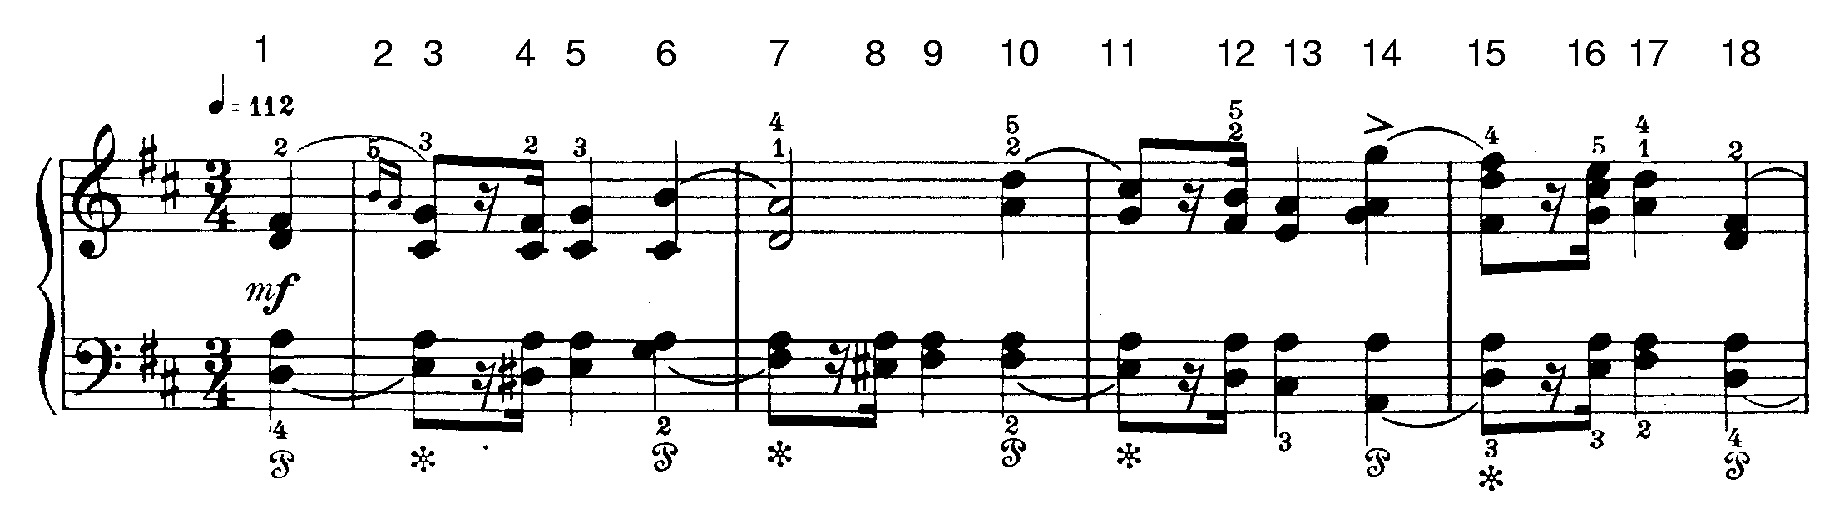
\includegraphics[width=\IPEMDefaultFigureWidth]{Graphics/SchumannScore}
    \caption{The first four measures of Schumann's piece "Kuriose Geschichte"}
    \label{Fig:SchumannScore}
\end{figure}

\begin{figure}[h]
    \centering
    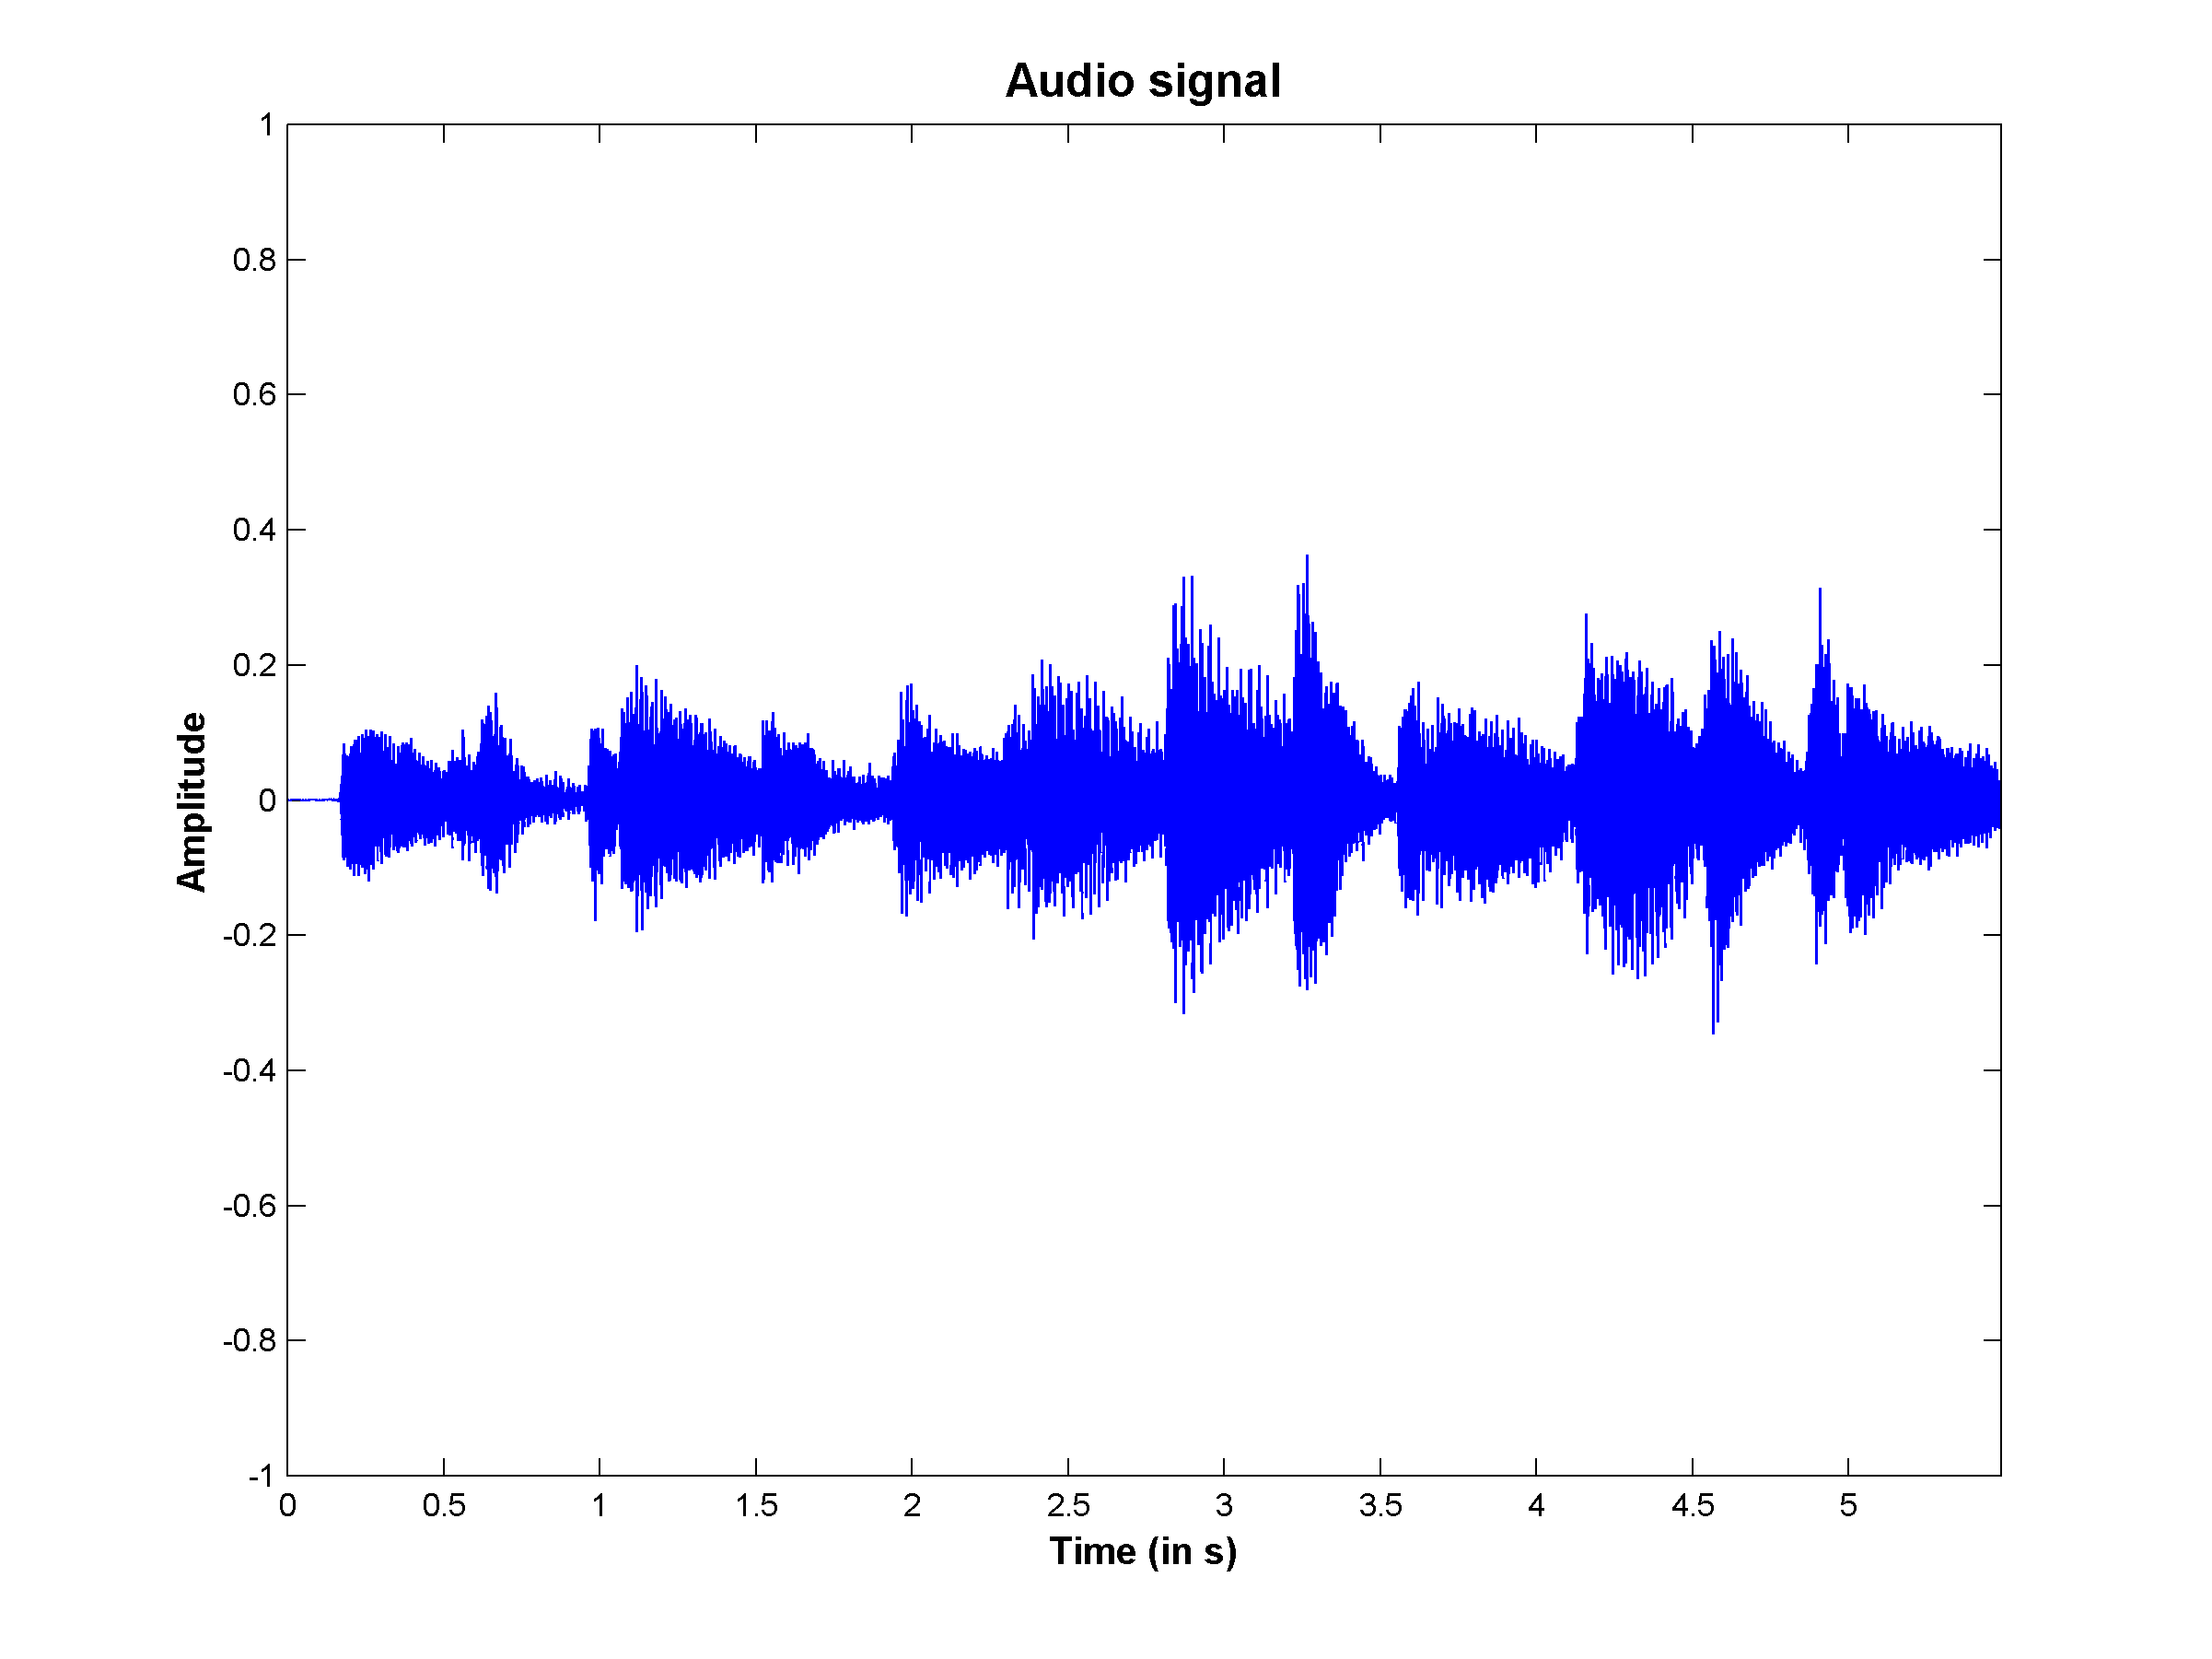
\includegraphics[width=\IPEMDefaultFigureWidth]{Graphics/SchumannAudioSignal}
    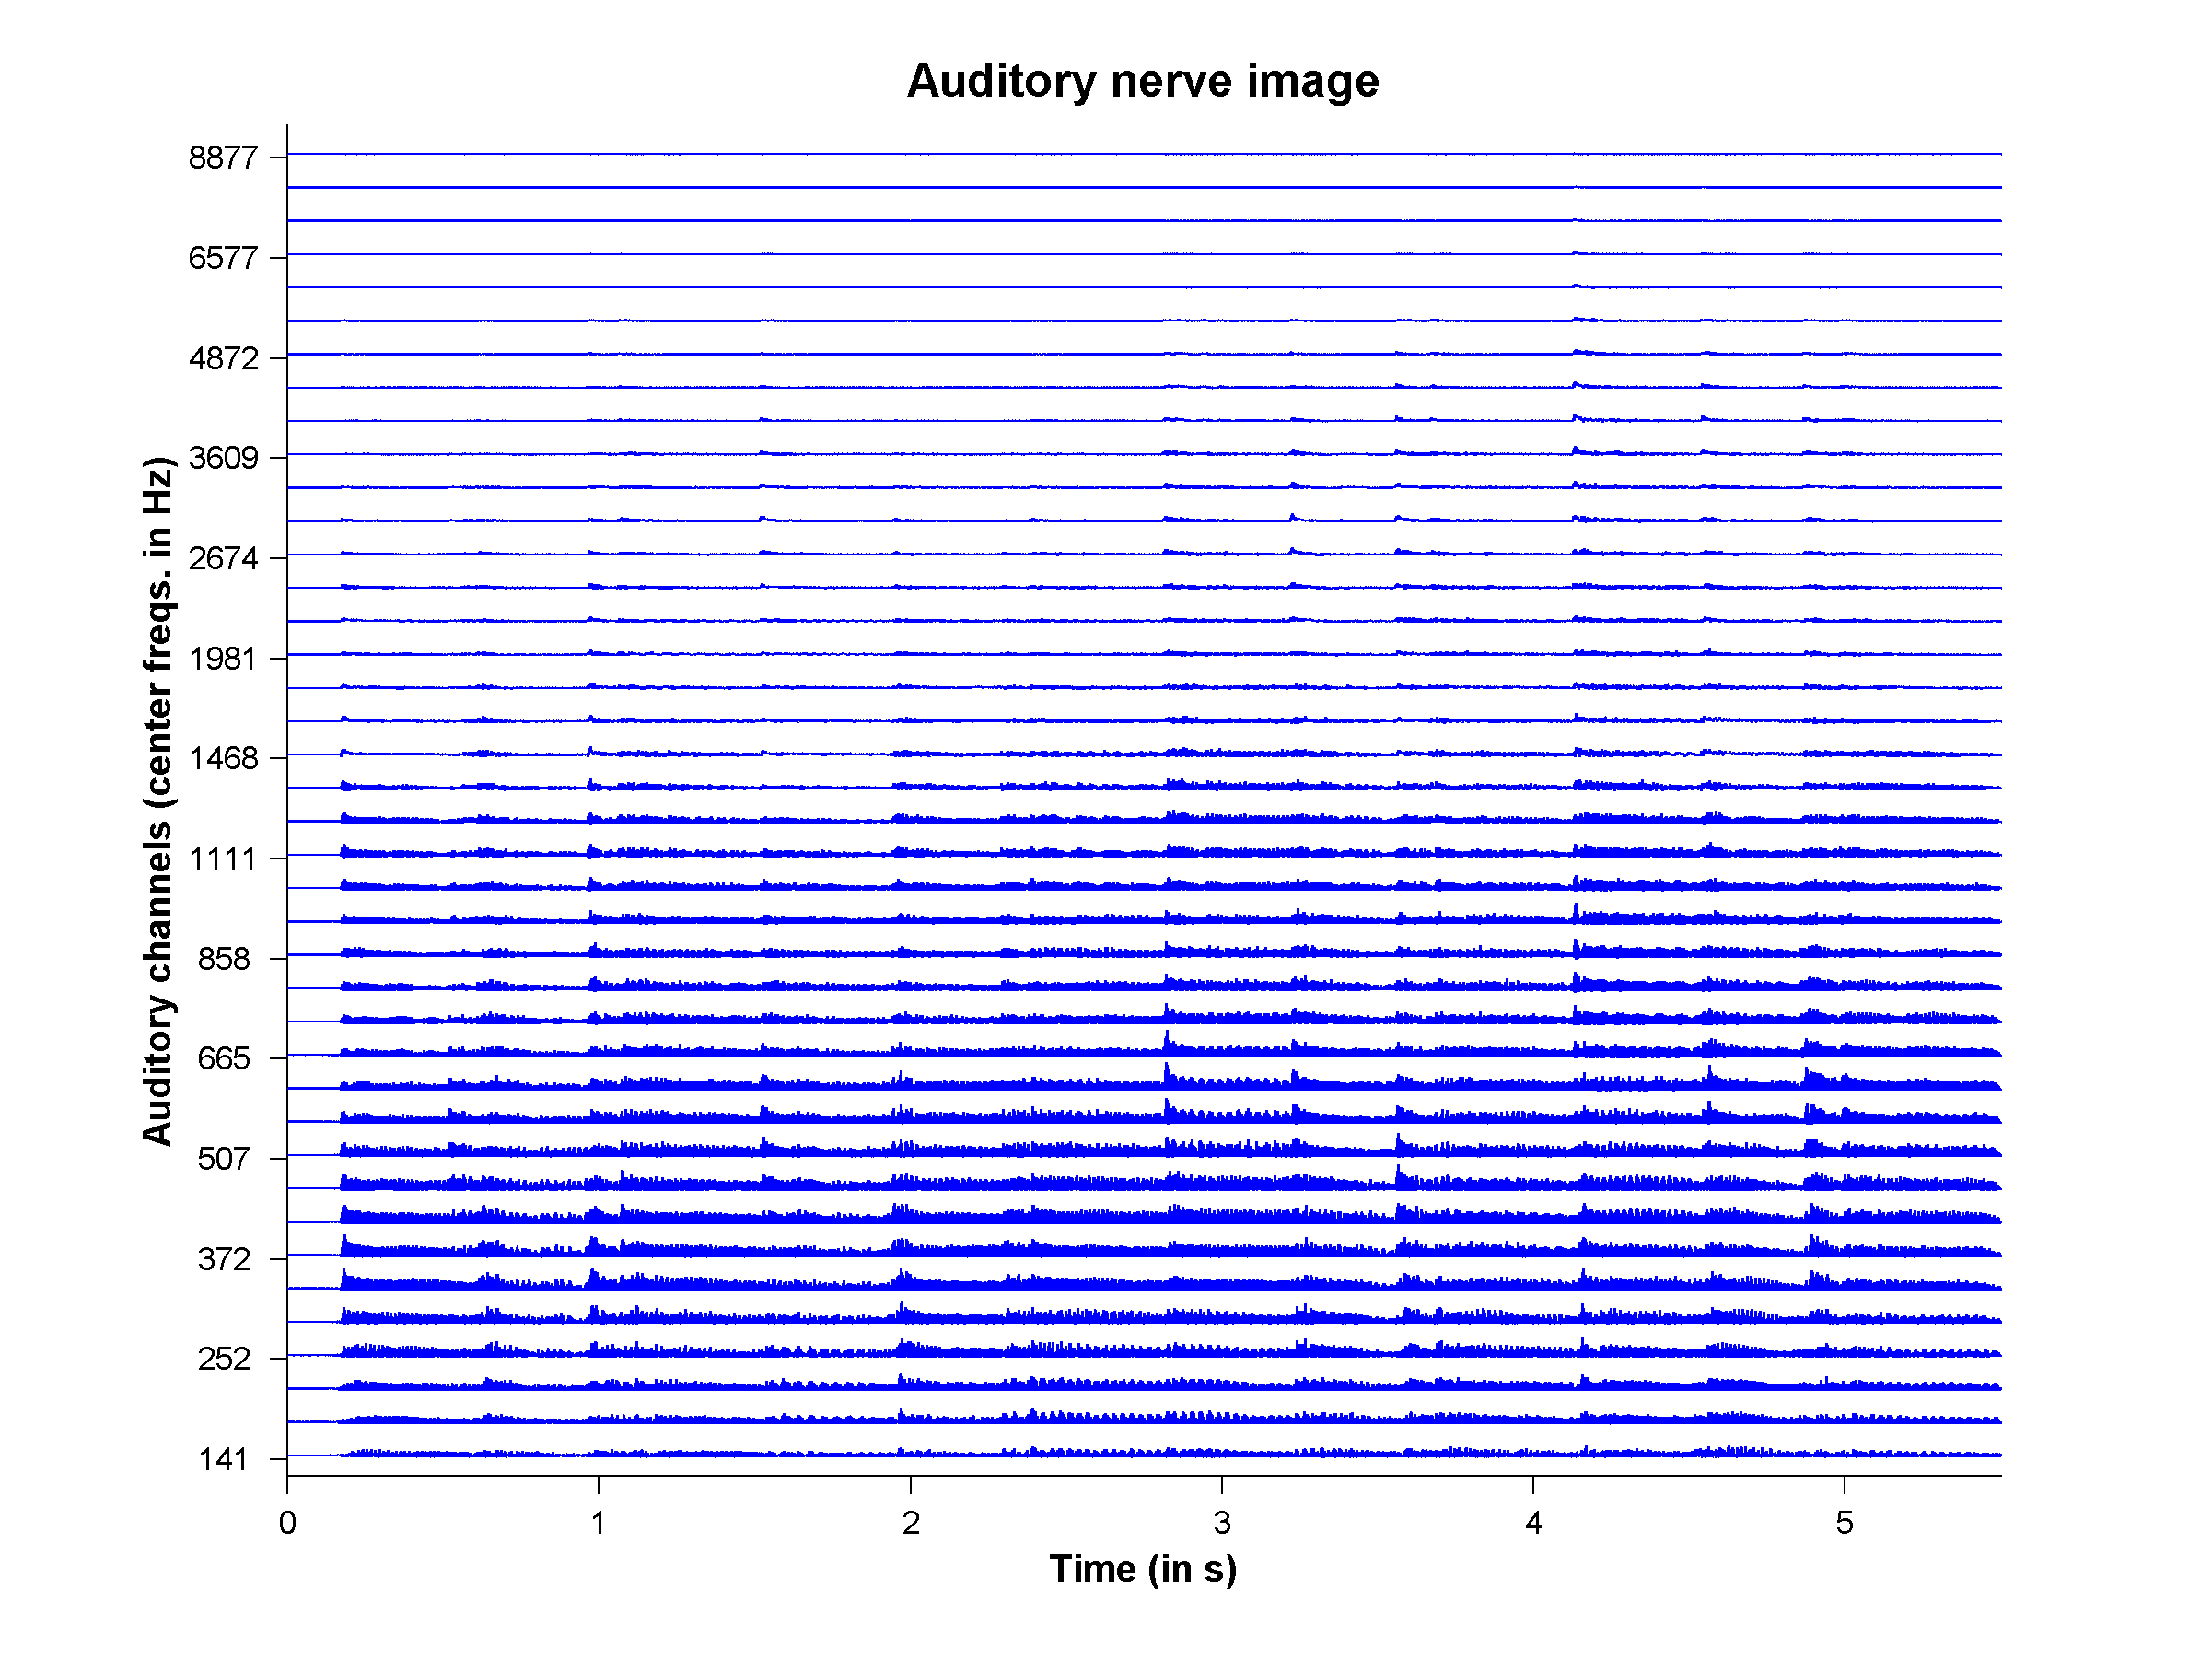
\includegraphics[width=\IPEMDefaultFigureWidth]{Graphics/SchumannANI}
    \caption{Top: waveform of a short excerpt of Schumann's Kuriose Geschichte. Bottom: primary image}
    \label{Fig:SchumannANIandAudioSignal}
\end{figure}

\begin{figure}[h]
    \centering
    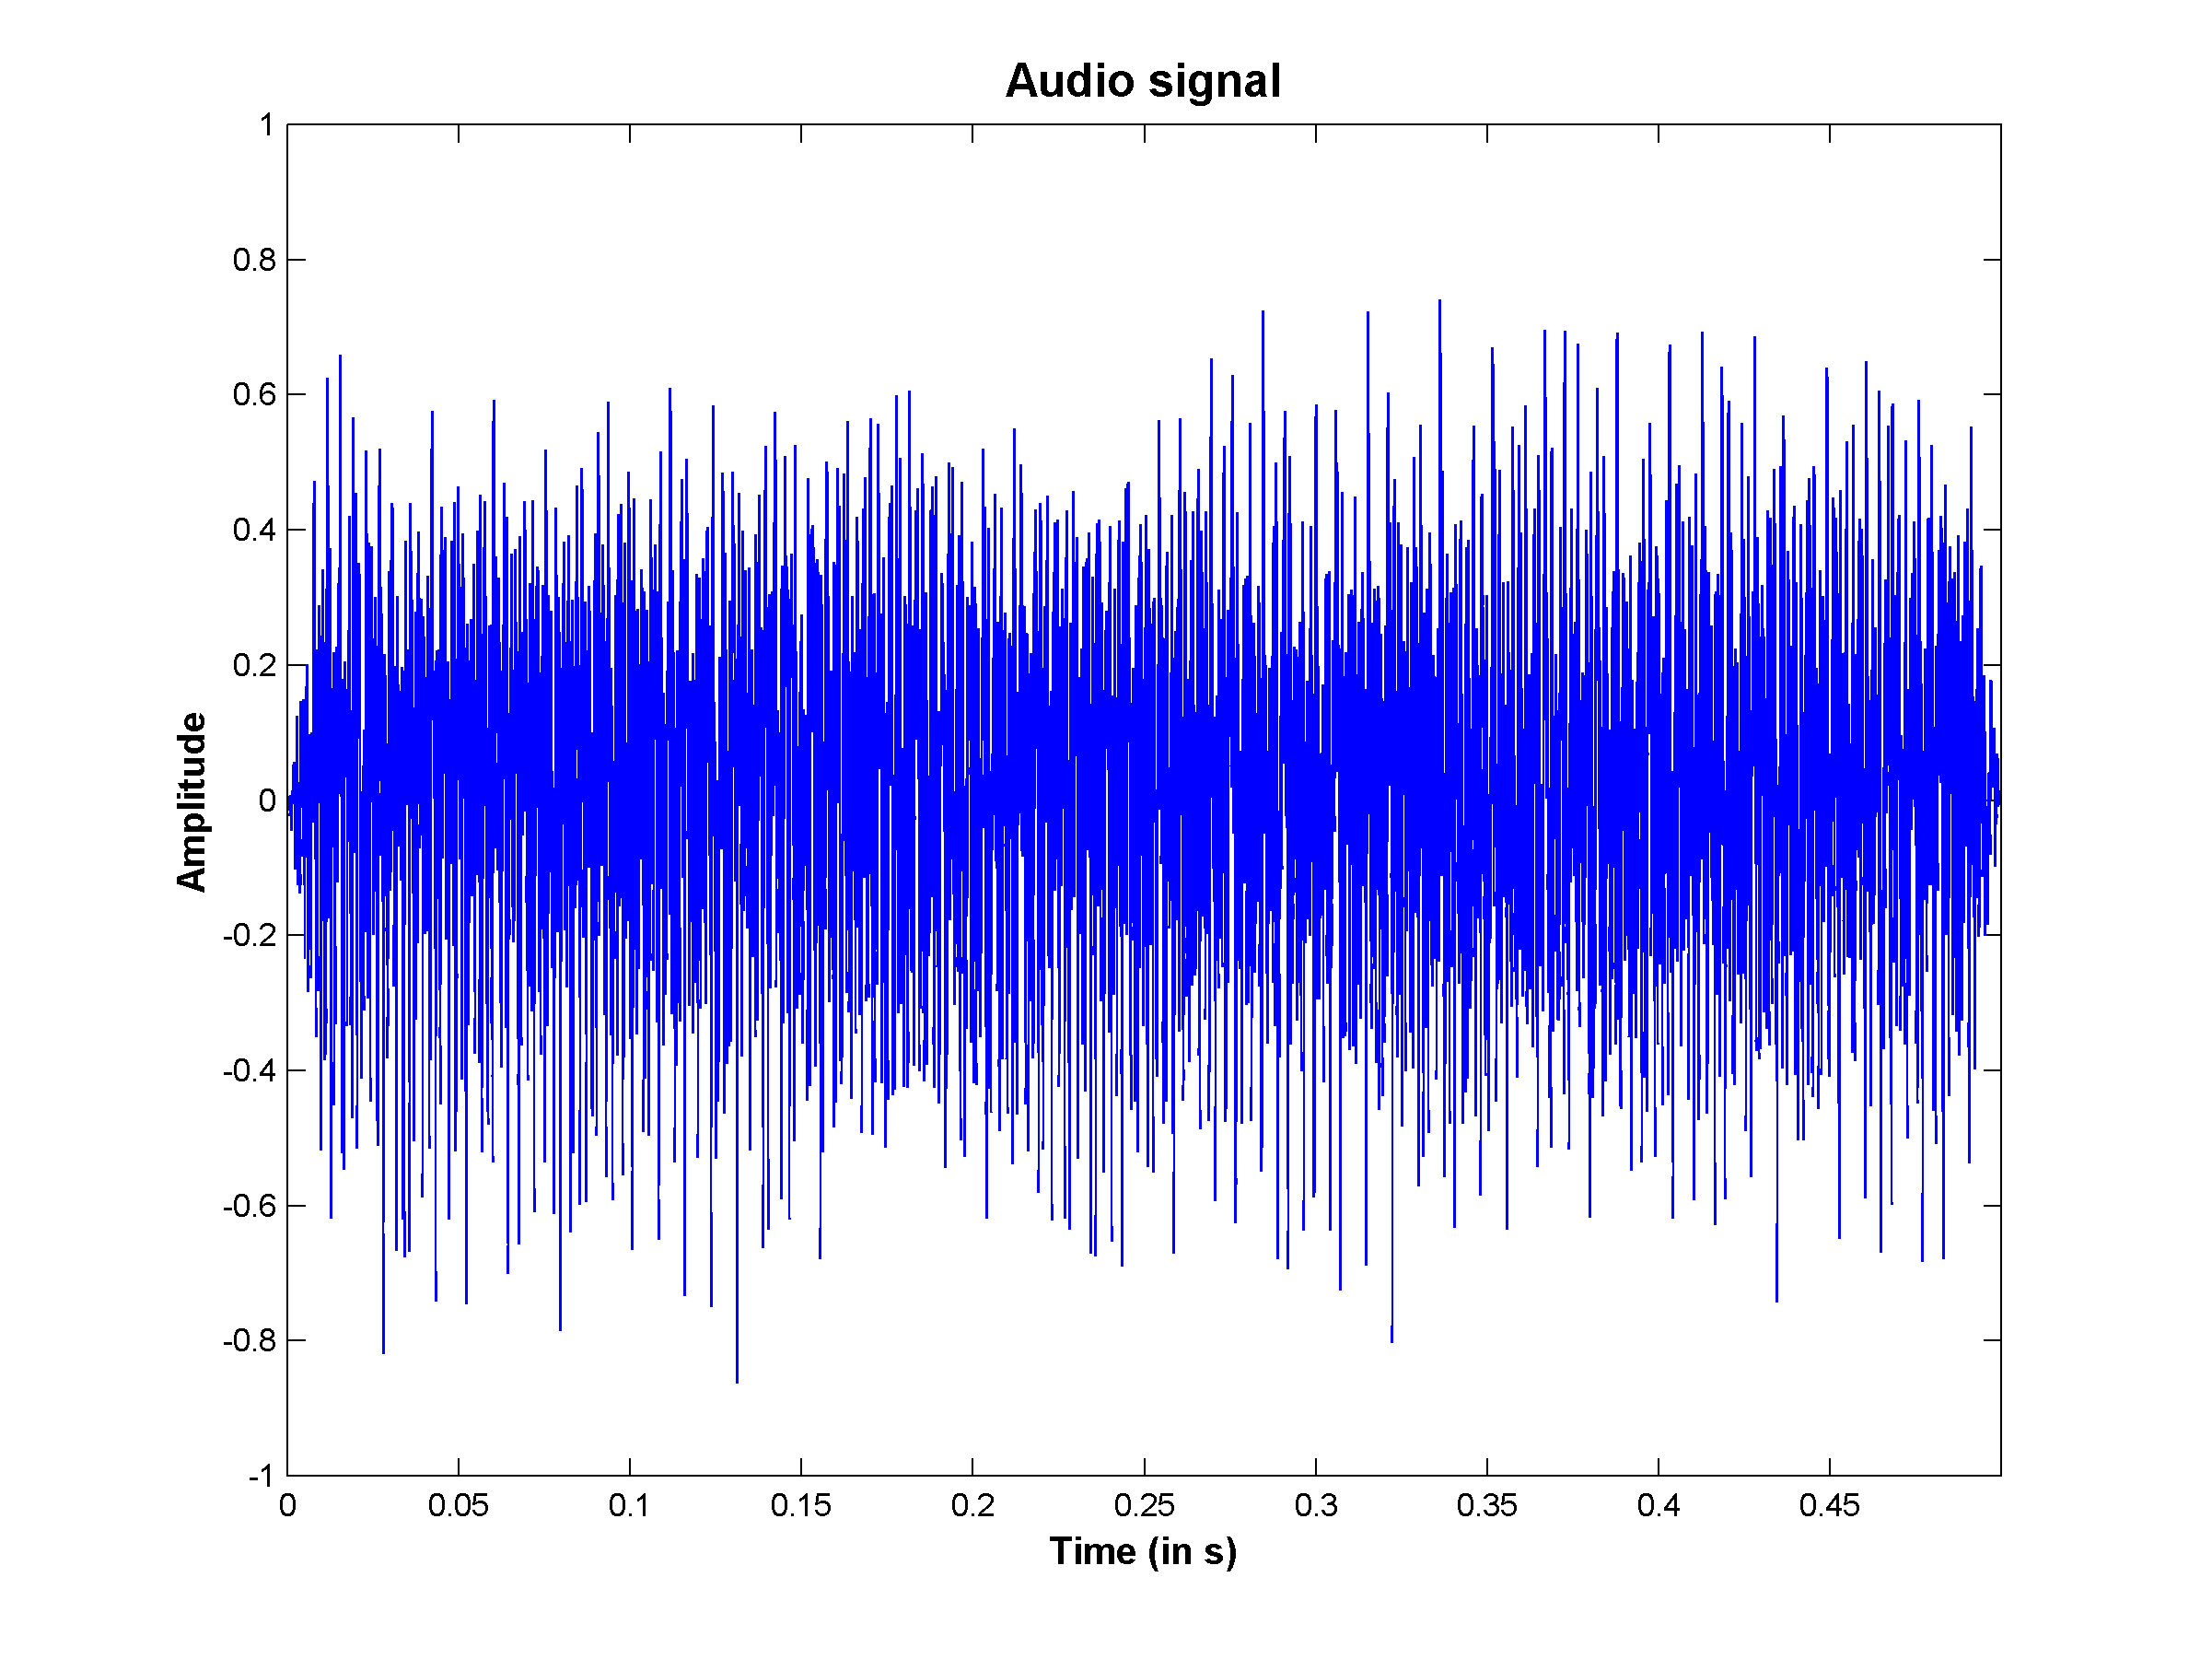
\includegraphics[width=\IPEMDefaultFigureWidth]{Graphics/ShepardCChordAudioSignal}
    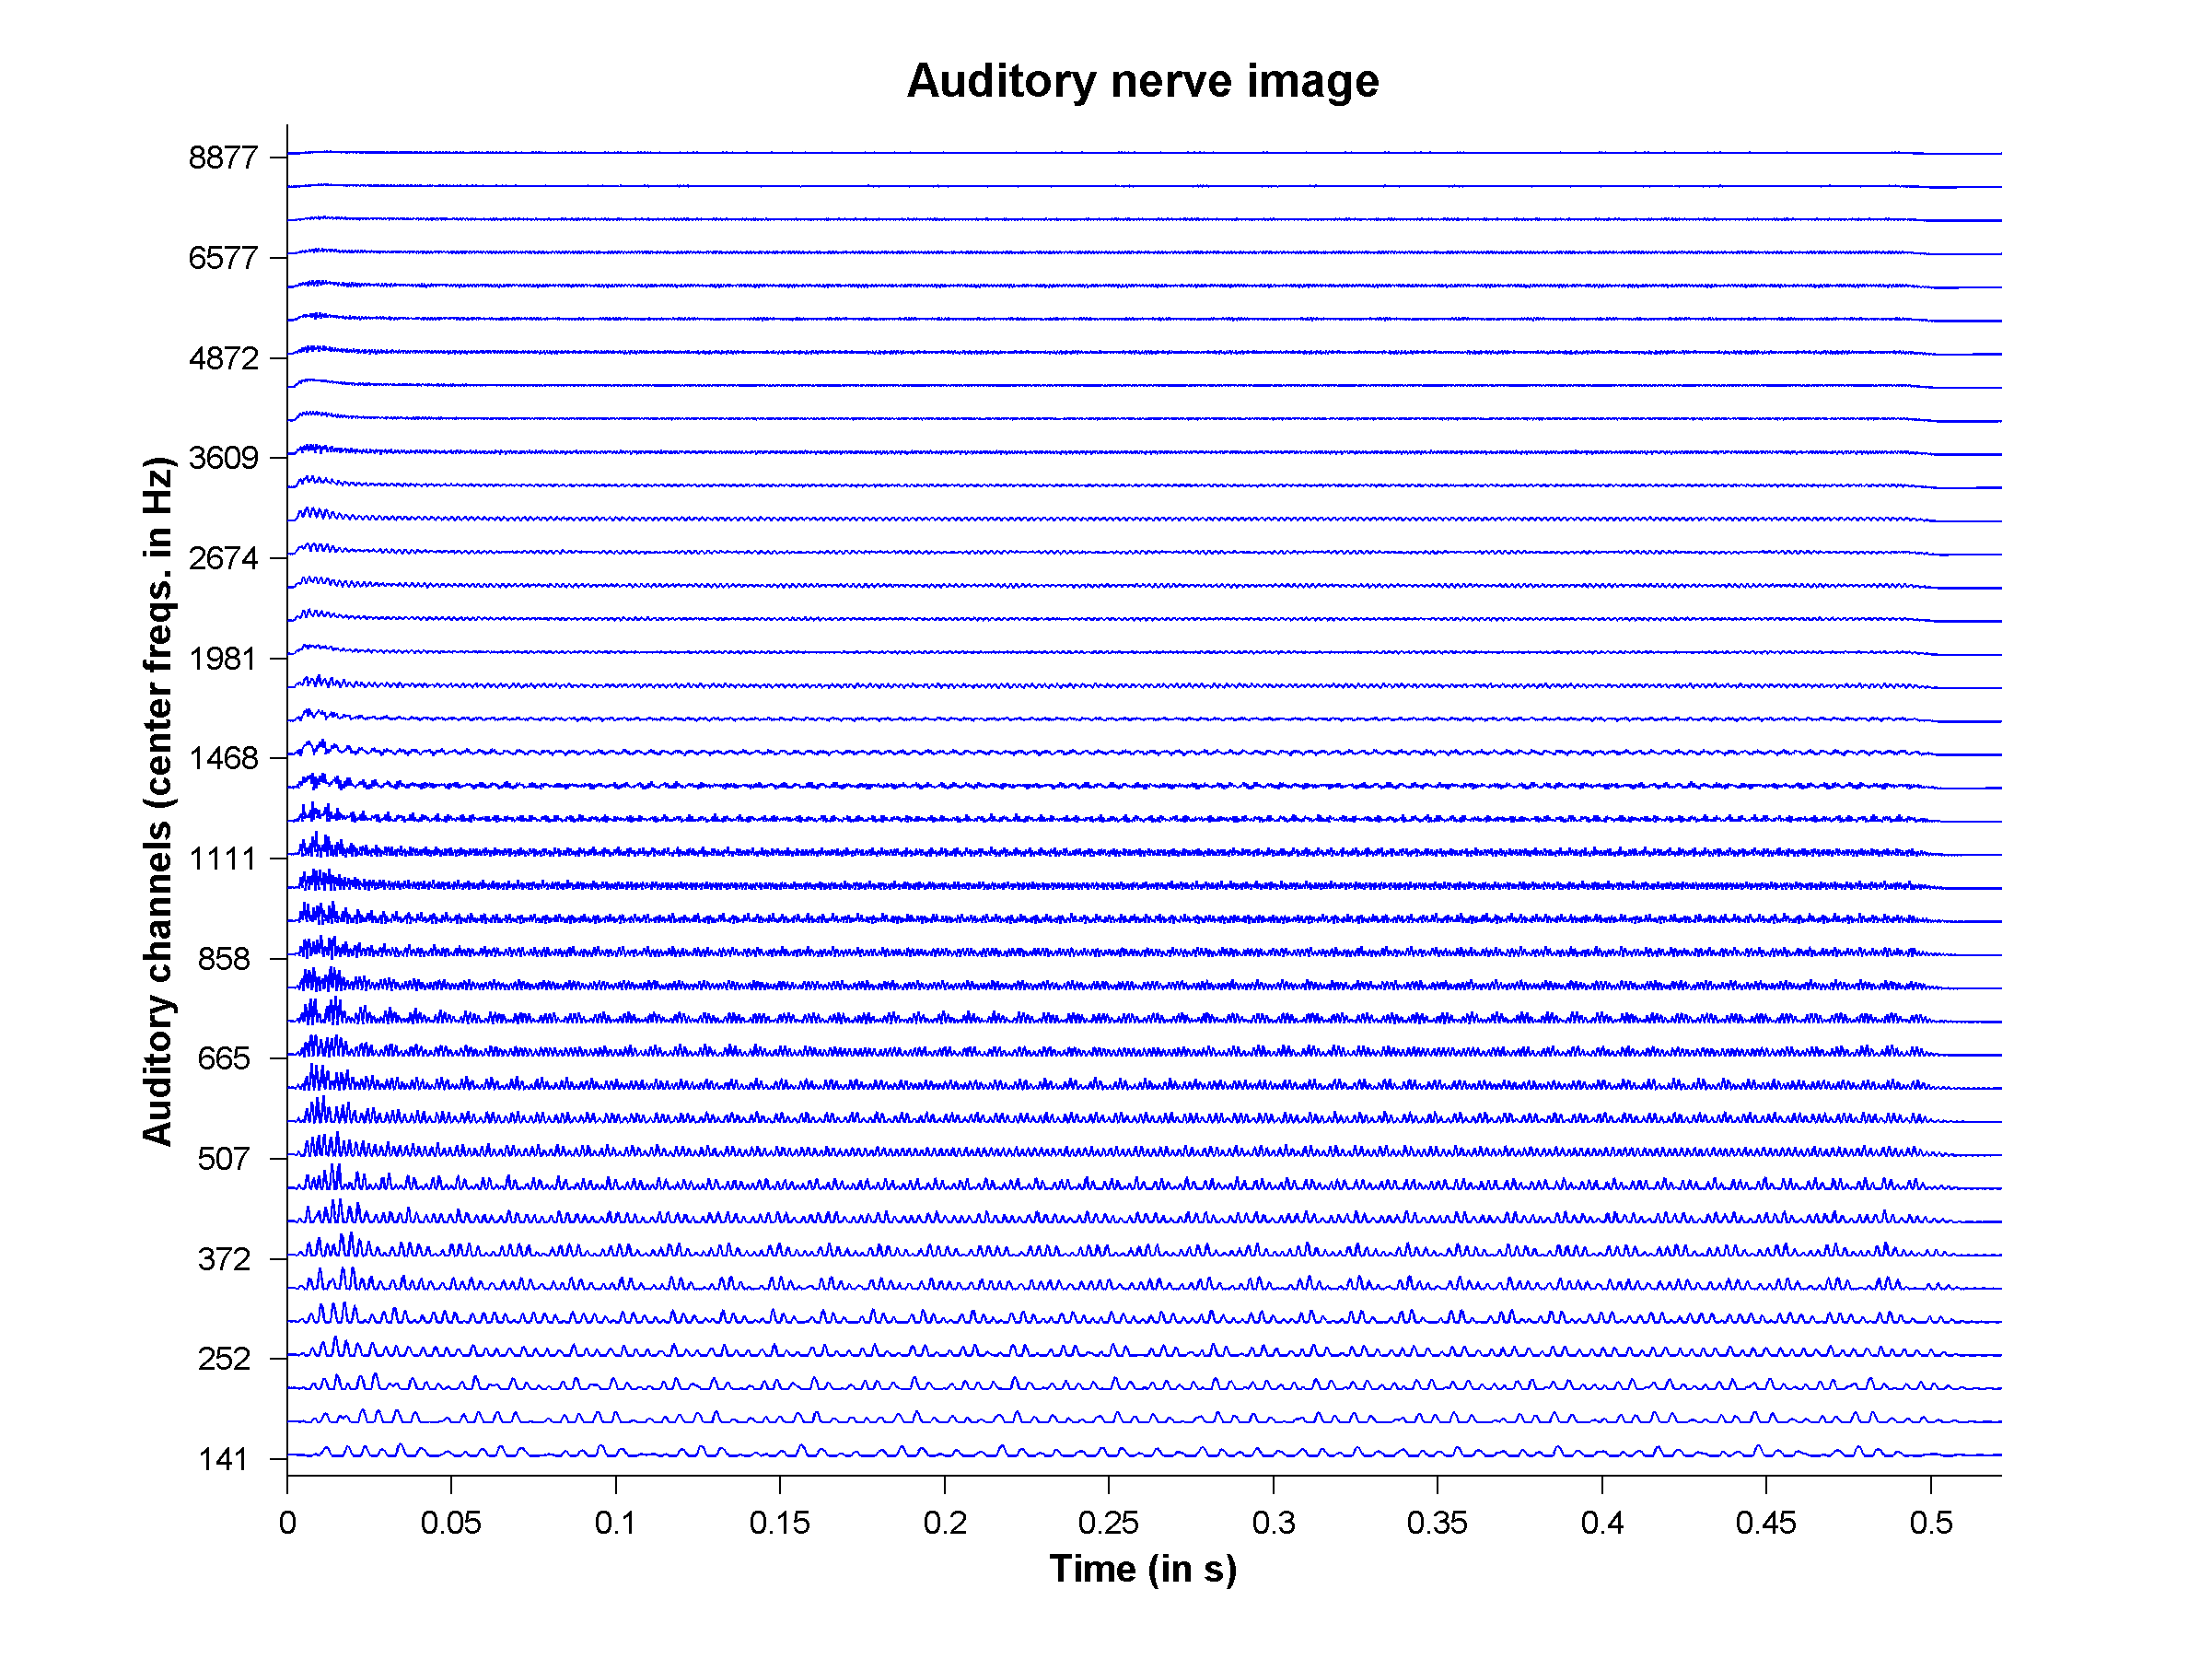
\includegraphics[width=\IPEMDefaultFigureWidth]{Graphics/ShepardCChordANI}
    \caption{Top: waveform of a C major chord using Shepard tones. Bottom: primary image}
    \label{Fig:ShepardCChordANIandAudioSignal}
\end{figure}

% --------------------------------------------------------------------------------

% --------------------------------------------------------------------------------
% --------------------------------------------------------------------------------
\newpage
\section{Roughness Module}
% --------------------------------------------------------------------------------

% Make general target
\hypertarget{Concepts:RoughnessModule}{}

% Make target for following functions:
\hypertarget{Concepts:IPEMRoughnessFFT}{}

\subsection{Introductory description}
% --------------------------------------------------------------------------------

The Roughness Module (RM) calculates the roughness (or
equivalently: the sensory dissonance) of a sound. Roughness is
considered to be a sensory process highly related to texture
perception. Hence, in our global chart of image transformation
modules it is localized in the top left (texture and sensory
based) section of figure \ref{Fig:ModulesRM}.
\begin{figure}[h]
    \centering
    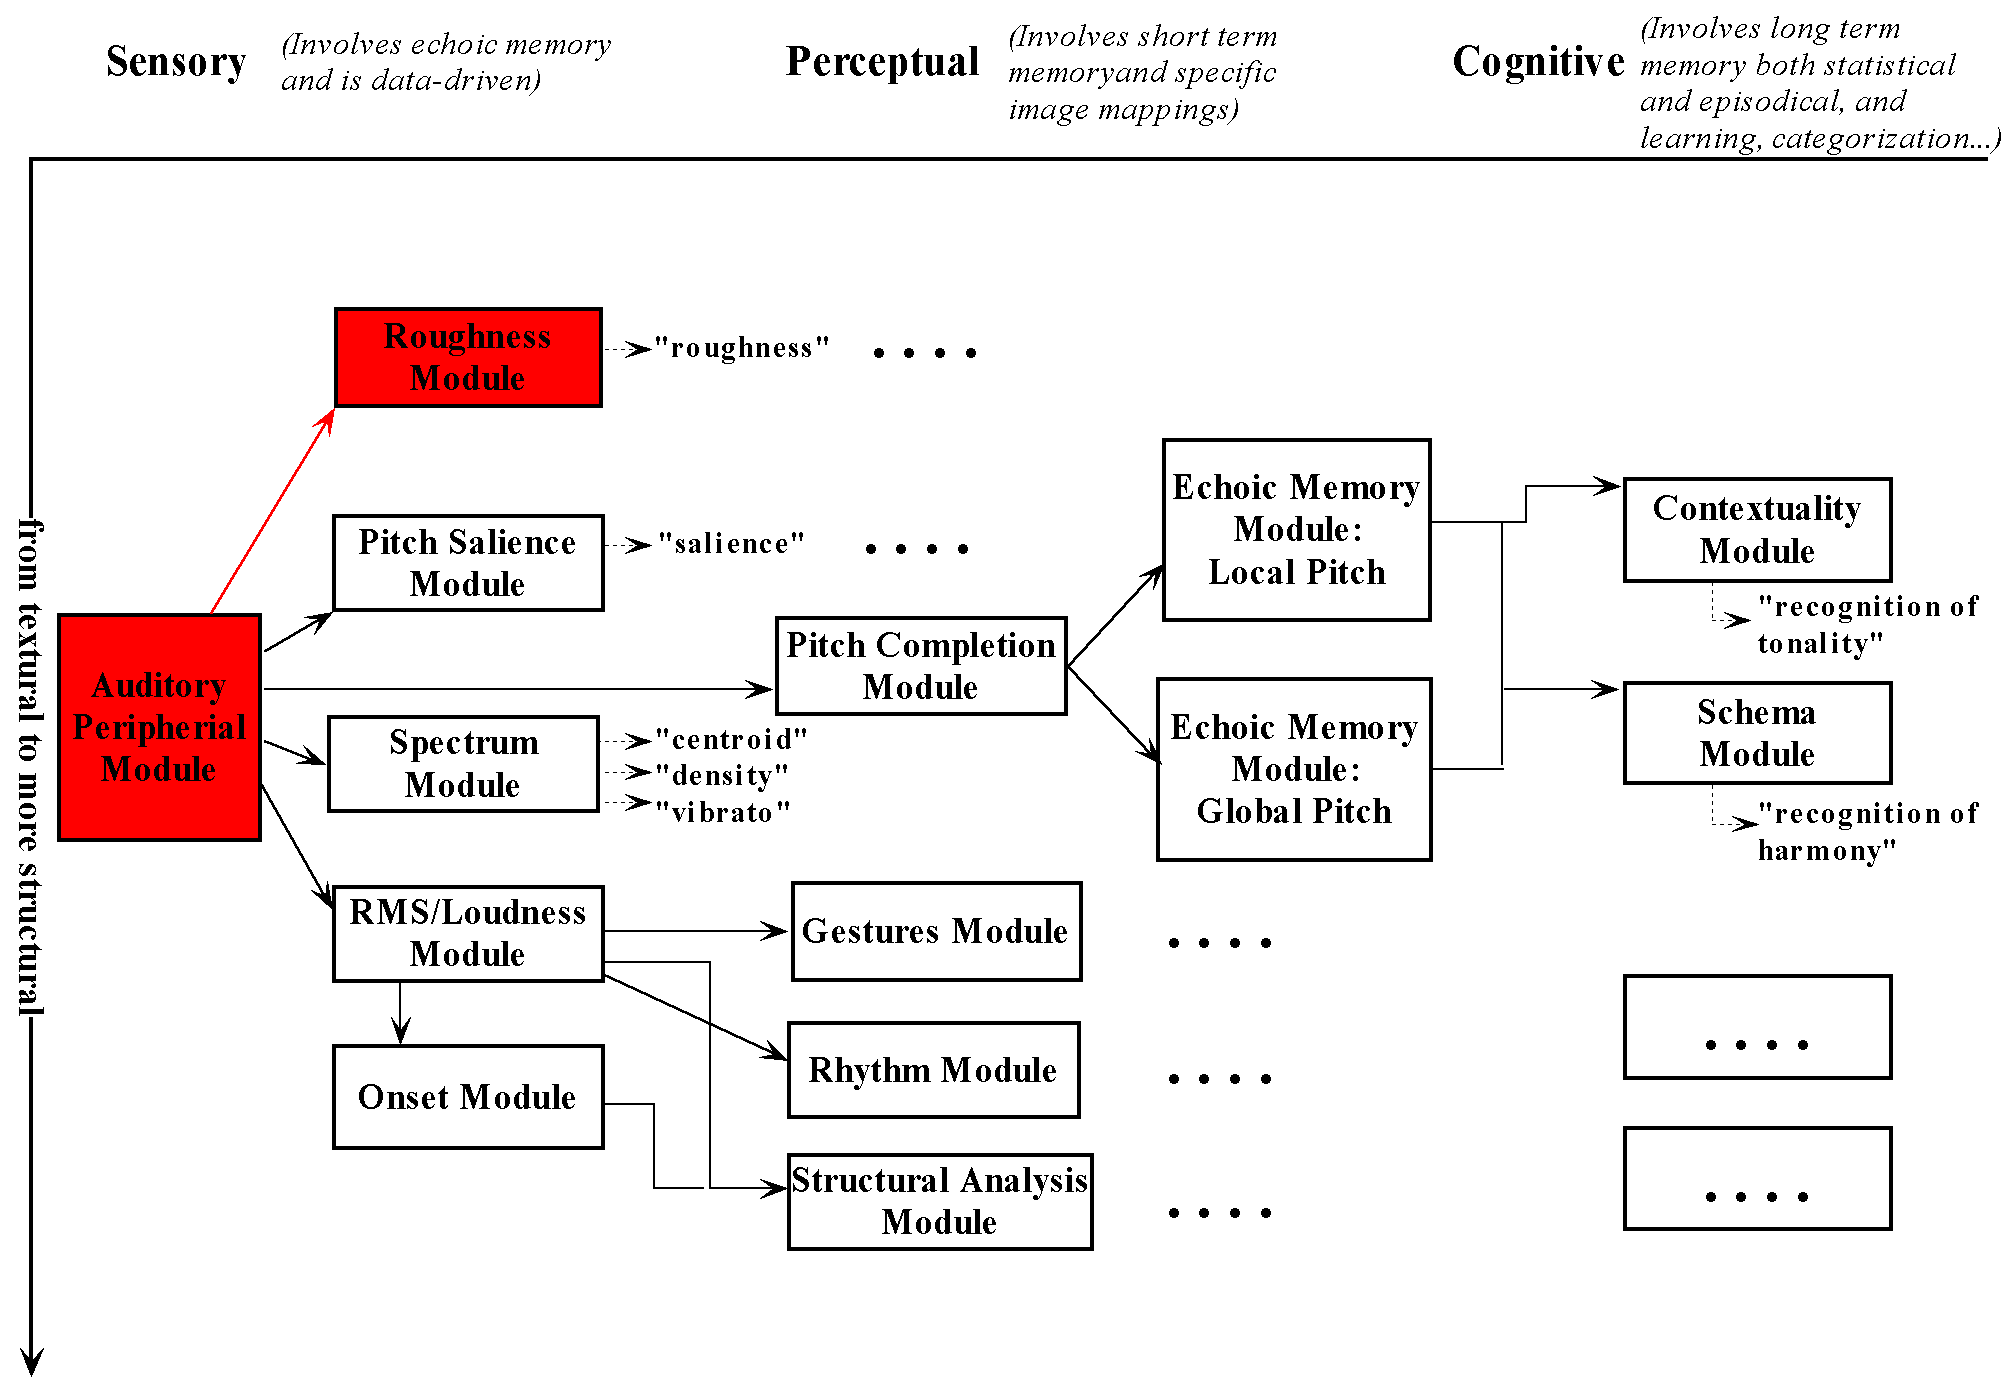
\includegraphics[width=\textwidth]{Graphics/ModulesRM}
    \caption{Chart of image transformation modules, with RM highlighted}
    \label{Fig:ModulesRM}
\end{figure}

The module takes sound as input (fig. \ref{Fig:RMModule}) and
produces a roughness estimation. The estimation should be
considered an inference.
\begin{figure}[h]
    \centering
    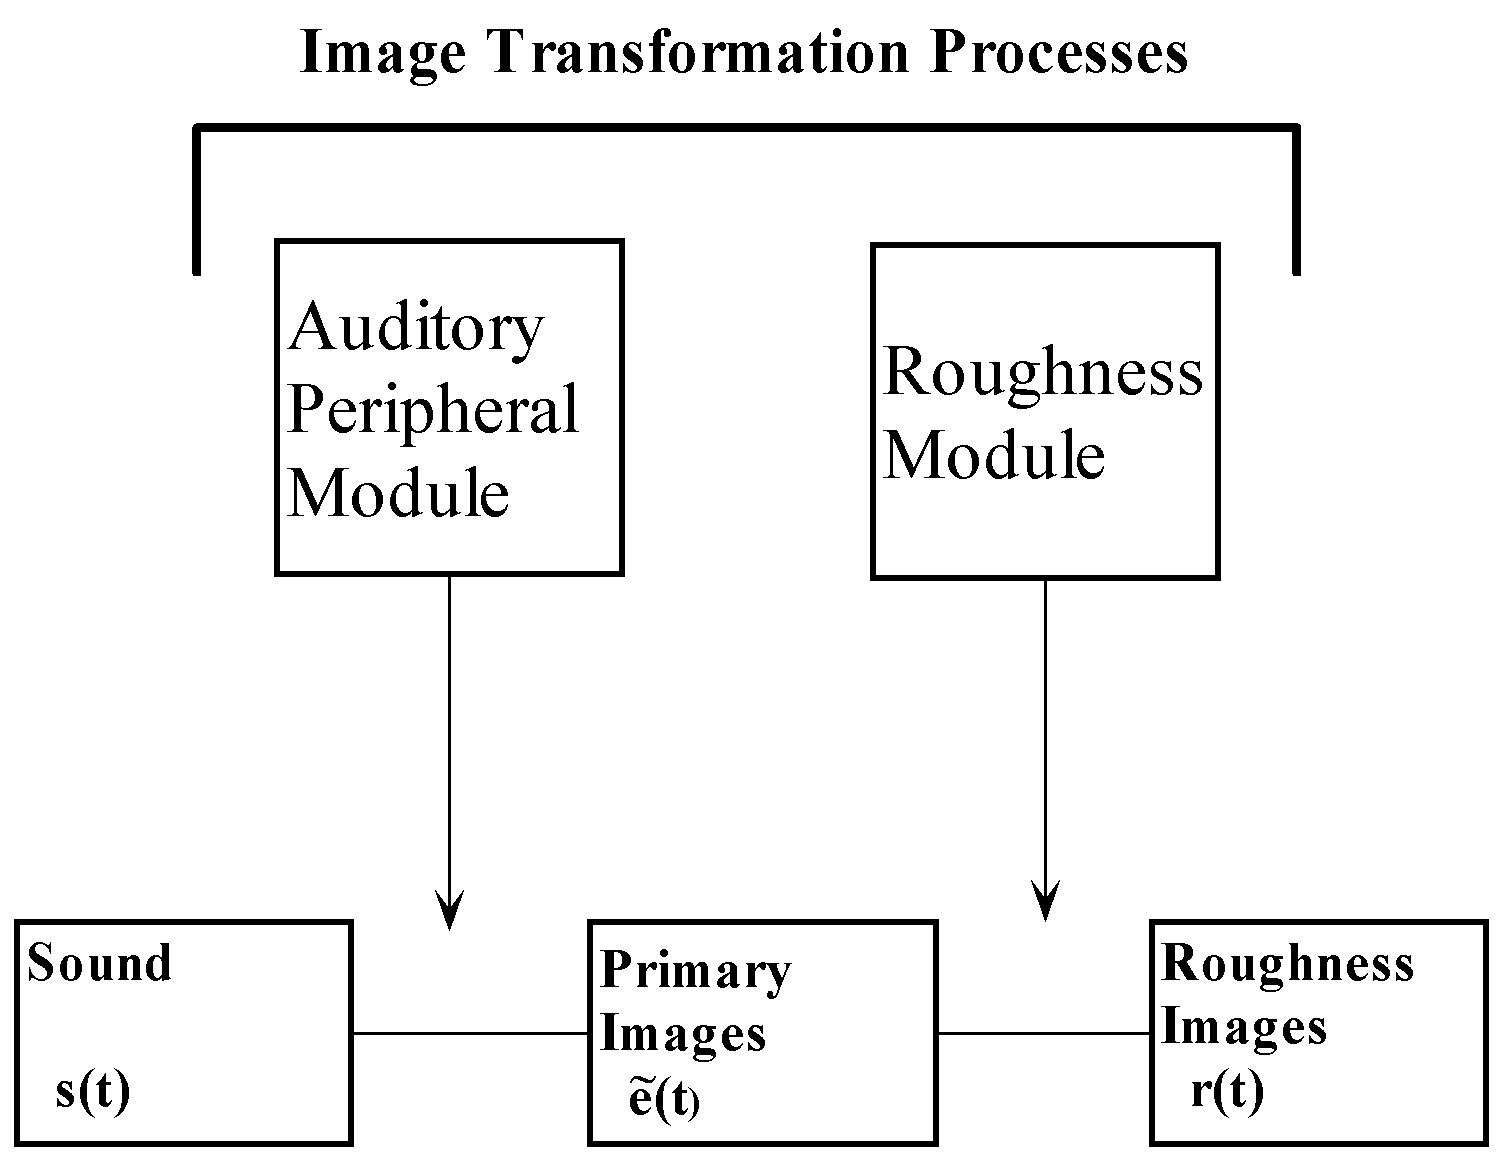
\includegraphics[width=\IPEMDefaultFigureWidth]{Graphics/RMModule}
    \caption{Image Transformation Process: Roughness Module}
    \label{Fig:RMModule}
\end{figure}
However, the module offers more than just an inference. The
visualization and calculation method of this module is based on
\citeA{inproceedings:Leman:DAFx:2000} where roughness is
defined as the energy of the relevant beating frequencies in the
auditory channels. The model is called the synchronization index
model of roughness and it is based on phase-locking to frequencies
that are present in the neural patterns. The synchronization index
model allows a straightforward visualization of the energy
components underlying roughness, in particular (i) with respect to
auditory channels, and (ii) with respect to phase-locking
synchronization (= the synchronization index for the relevant
beating frequencies on a frequency scale). That's why it is more
than just an inference. It assumes that neurons somehow extract
the energy of the beating frequencies and form internal images on
which the inference is based.

But what are beating frequencies? Take an amplitude modulated sine
wave with carrier frequency $f_c$ and modulation frequency $f_m$.
Such a signal has only three frequencies in the spectrum, in
particular $f_c$, $f_c-f_m$, and $f_c+f_m$. The beating frequency
is $f_m$. Now, in the auditory system, these frequencies are
introduced as effective beating frequencies into the spectrum of
the neural rate-code patterns. This is due to wave rectification
in the cochlea where the lower part of the modulated signal is cut
off, and as a result new frequencies are introduced of which the
most important ones correspond with the beating frequency $f_m$
and its multiples. As a matter of fact, neurons may synchronize
with these frequencies provided that they fall in the frequency
range where synchronization is physiologically possible. This
mechanism forms a physiological basis for the detection of beats
and hence, the sensation of roughness.

According to \citeA[p.~520-521]{Javel:88}, the synchronization
index represents the degree of phase-locking to a particular
frequency that is present in the neural pattern. The index can be
mathematically expressed as the (normalized) Fourier Series
coefficient at the frequency of interest. Using this concept, the
degree of roughness can be defined as the sum of the normalized
magnitudes or 'energies' of the relevant beating frequencies in
the Fourier spectrum.


\subsection{Functional-logical description}
% --------------------------------------------------------------------------------

Strictly speaking the roughness module realizes a transformation
from auditory nerve images onto roughness values. In a broad sense
the module starts from sound involving:
\begin{eqnarray}
    APM: s(t) \rightarrow \tilde{e}(t)\\
    RM: \tilde{e}(t) \rightarrow r(t)
\end{eqnarray}
where APM is the Auditory Peripheral Module which is used as the
first step, and RM is the transformation from the primary images
$\tilde{e}(t)$ to the roughness values $r(t)$ (our Roughness
Module in the strict sense). The latter are scalar values which we
can compare with human behavioral outputs.

\subsection{Signal processing description}
% --------------------------------------------------------------------------------

The synchronization index model calculates roughness in terms of
the 'energy' of neural synchronization to the beating
frequencies. The 'energy' refers to a quantity which we derive
from the magnitude spectrum.

Since the beating frequencies are contained in the lower
spectral area of the neuronal pattern $e(t,c)$, the spectral
part we are interested in is defined as:
\begin{equation}
  B(t,f,c) ~=~ F(f,c)D(t,f,c)
\end{equation}
where $F(f,c)$ is a filter whose spectrum is depending on the
channel $c$, and $D(t,f,c)$ is the short-term spectrum in
channel $c$ which we define as:
\begin{equation}\label{E1}
  D(t,f,c)~=~\int_{-\infty}^{+\infty} e(t,c)w(t'-t)e^{-j2\pi
  ft'}~dt'
\end{equation}
where $e(t,c)$ is the neural pattern in channel $c$, and
$w(t'-t)$ is a (hamming) window. The \emph{magnitude} spectrum
is then defined as $\left|~D(t,f,c)~\right|$, and the
\emph{phase} spectrum as $\angle D(t,f,c)$.

In order to be able to reproduce the psychoacoustical data on
roughness, the filters $F(f,c)$ should be more narrow at auditory
channels where the center frequency is below 800 Hz, and the
filters should be attenuated for high center frequencies as
well. The proposed set of filters $F(f,c)$ are shown in figure
\ref{Fig:Filters}. Small changes in parameters do not have a
dramatic effect on the performance of the model.

\begin{figure}[ht]
    \centering
    \includegraphics[width=\IPEMDefaultFigureWidth]{Graphics/Filters}
    \caption{Filters become more narrow in the lower auditory channels.}
    \label{Fig:Filters}
\end{figure}



$B(t,f,c)$ represents the \emph{spectrum} of the neural
synchronization to the beating frequencies in channel $c$. The
\emph{synchronization index} of the beating frequencies is then
defined as the normalized magnitude:
\begin{equation}
  I(t,f,c) ~=~ \left |~ \frac{B(t,f,c)}{D(t,0,c)}~\right |
\end{equation}
where $I(t,f,c)$ is the normalized magnitude in channel $c$.
$D(t,0,c)$ is the DC-component of the whole signal in channel
$c$.

The short-term \emph{'energy'} spectrum of the neural
synchronization to beating frequencies in a particular auditory
channel $c$ is defined as:
\begin{equation}\label{Rspectrum}
\textbf{B}(t,f,c) ~=~ I(t,f,c) ~^{1.6}~=~ {\left |~
\frac{B(t,f,c)}{D(t,0,c)}~\right |~}^{1.6}
\end{equation}

%\item
% the energy spectrum of the neural synchronization to
% beating frequencies over all auditory
% channels is:
%\begin{equation}\label{R2}
%\textbf{B}(t,f) ~=~ \sum_{c=1}^{C} \textbf{B}(t,f,c)~ w_c
%\end{equation}
%where $w_c$ is the weighting factor defined for each channel.
%\item
% the overall energy of the neural synchronization to beating frequencies in one channel is:
% \begin{equation}\label{R3}
%E_\textbf{B}(t,c) ~=~ \int_{f=-\infty}^{+\infty}
%\textbf{B}(t,f,c)~df
%\end{equation}
%\end{itemize}



We then define the following relationships for the calculation of
roughness:
\begin{equation}\label{R5}
\begin{array}{lll}
  R_\textbf{B}(t)&~=~\int \textbf{B}(t,f)~df
                 &~=~\int \sum_{c=1}^{C}
                 \textbf{B}(t,f,c)~df\\\\
                 &~=~\sum_{c=1}^{C} \textbf{B}(t,c)
                 &~=~\sum_{c=1}^{C} \int  \textbf{B}(t,f,c)~df\\
\end{array}
\end{equation}
where $R_\textbf{B}(t)$ is the roughness at time $t$. The
roughness is obtained by an integration of the 'energy' over all
frequencies, as well as over all channels. This definition
implies a proper visualization, one along the axis of auditory
channels and one along the axis of the (beating) frequencies.

%We now assume that roughness is related to the 'energy' of this
%normalized Fourier transform.
%
%In particular, roughness is calculated in the individual channels
%and the total roughness is the sum of the channel roughnesses.
%Given the above discussion, it will be possible to visualize the
%contribution of the synchronization energy along the axis of the
%auditory channels, as well as along the axis of the beating
%frequencies.






%Given the general concept as described above, the implementation
%requires a specification of the filters $F(f,c)$. In the present
%modeling, we choose elegance as an important criterium to
%describe the filters mathematically.
%The form of the filter
%$F'(f,c)$ has first been defined according to the following
%formula's:
%\begin{equation}
%F'(f,c)~=~e^{-8 \frac{f}{f_B}} \left [~1 - cos(2 \pi
%\frac{f}{10f_B}) ~\right ] w(c)
%\end{equation}
%where $f_B$ is the frequency range of the filter and $f$ is
%running from 1 to $f_B$, $w(c)$ is a weight depending on the
%channel $c$. The weight takes into account a linear decrease of
%the impact of the filter depending on the auditory channel number:
%\begin{equation}
%w(c)~=~1-\frac{0.55c}{C})
%\end{equation}
%with c running from 1 to C (=40). The frequency range $f_B$ is
%defined such that it is narrow for the lower auditory channels
%below 800 Hz, broad at about 1000 Hz and again slightly more
%narrow at frequencies higher than 1500 Hz.
%
%A sigmoid function has been defined according to
%%(fig.~\ref{Sigmoid}):
%\begin{equation}\label{Sigmoid}
%S~=~ \frac{(\frac{c}{C})^{.2}} {0.04 + (\frac{c}{C})^{2.45} -
%0.007c}
%\end{equation}
%The sigmoid function is used to define the frequency range as:
%\begin{equation}
%f_B(c) = 10 + (300 * \frac{S}{S_{max}} );
%\end{equation}
%It means that the frequency range of the filter in the lowest
%auditory channel is 10 Hz, and that this range is at most 310 Hz
%(around 1000 Hz). The values of S are normalized so that the
%maximum value of $\frac{S}{S_{max}}$ is equal to one.
%
%%\begin{figure}
%%  \centering
%%  \includegraphics{figures/Sigmoid}
%%  \caption{Sigmoid function}\label{Sigmoid}
%%\end{figure}
%Given the set of filters $F(f,c)$, the sigmoid function
%(\ref{Sigmoid}) has also been used to define where the maximum of
%the filter should be located. Data indicate that the maximum
%around 1000 Hz is at about 70 Hz. It is lower for low auditory
%channels.
%\begin{equation}
%f_M(c) = 20 + (52 * \frac{S}{S_{max}} );
%\end{equation}
%This function starts at 20 Hz and the maximum is obtained at 72
%Hz.
%
%The precise location of the filter shape $F'(f,c)$ on the
%frequency axis is then determined by placing its maximum at
%$f_M(c)$.



%Figure \ref{Filters} shows an array of such filters.
%\begin{figure}
%  \centering
%  \includegraphics{figures/Filters}
%  \caption{Filters become more narrow in the lower auditory channels}\label{Filters}
%\end{figure}


\subsection{Implementation}
% --------------------------------------------------------------------------------

\begin{tabularx}{\linewidth}{llX}
\hyperlink{FuncRef:IPEMRoughnessFFT}{IPEMRoughnessFFT} & - & Calculates roughness using synchronization index model\\
\end{tabularx}


\subsection{Examples}
% --------------------------------------------------------------------------------

The function
\hyperlink{FuncRef:IPEMRoughnessFFT}{IPEMRoughnessFFT}
has a number of input parameters. To calculate the roughness of
the wav-file \emph{SchumannKurioseGeschichte.wav} do:\\

\IPEMCodeExtract{[ANI,ANIFreq,ANIFilterFreqs] = ...\\IPEMCalcANIFromFile('SchumannKurioseGeschichte.wav');}\\

\IPEMCodeExtract{IPEMRoughnessFFT(ANI,ANIFreq,ANIFilterFreqs,5,300,0.200,0.020,1);}\\

Notice that the toolbox functions are linked through the variables
\IPEMCodeExtract{ANI,ANIFreq,ANIFilterFreqs}. These variables are
the output of the Auditory Peripheral Module, and (part of) the
input to the Roughness Module. The resulting figure should be
similar to the one shown in figure \ref{Fig:RMRoughness}.\\

\begin{figure}[h]
    \centering
    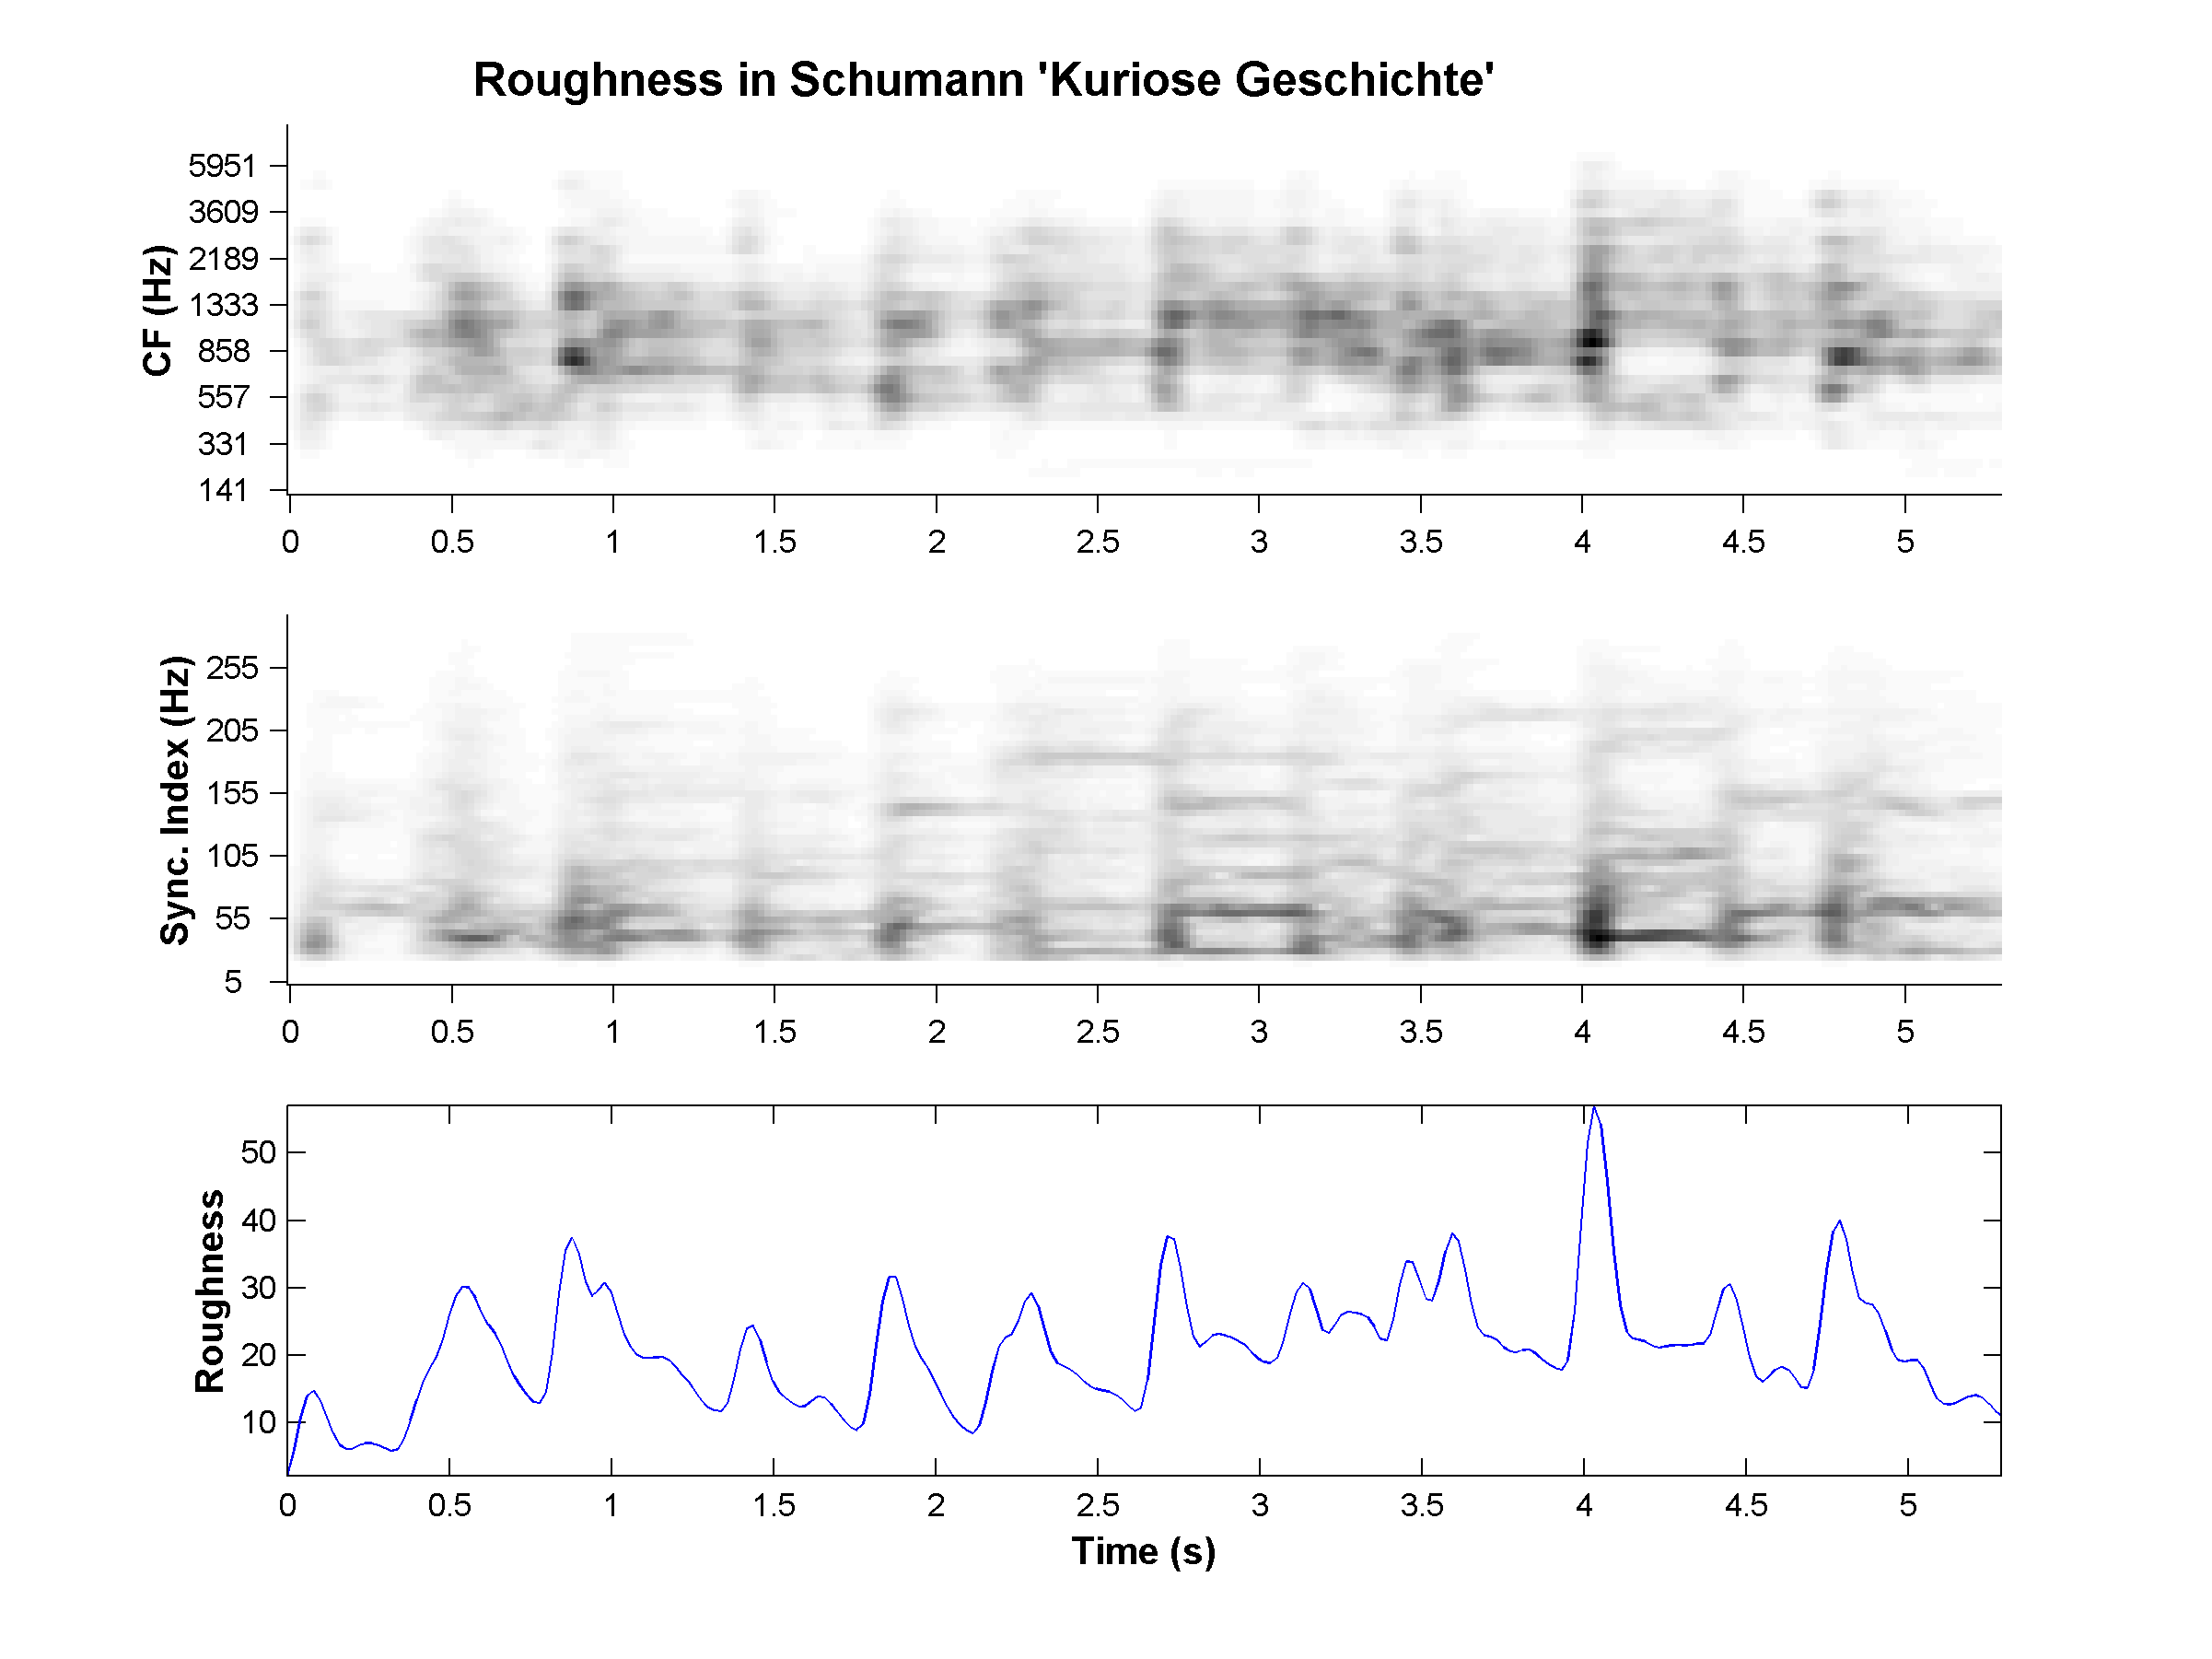
\includegraphics[width=\IPEMDefaultFigureWidth]{Graphics/RMRoughness}
    \caption{The upper panel shows the energy as distributed over the
    auditory channels, the middle panel shows the energy as
    distributed over the beating frequencies, the lower panel
    shows the roughness (which is the sum of either the upper or
    middle panel)}
    \label{Fig:RMRoughness}
\end{figure}

%See also \hyperlink{Chapter:ConceptsApplications}{Applications}
%for more elaborate examples.\\

% --------------------------------------------------------------------------------

% --------------------------------------------------------------------------------
% --------------------------------------------------------------------------------
\newpage
\section{Onset Module}
% --------------------------------------------------------------------------------

% Make general target
\hypertarget{Concepts:OnsetModule}{}

% Make target for following functions:
\hypertarget{Concepts:IPEMCalcOnsets}{}
\hypertarget{Concepts:IPEMCalcOnsetsFromANI}{}
\hypertarget{Concepts:IPEMDoOnsets}{}
\hypertarget{Concepts:IPEMOnsetPattern}{}
\hypertarget{Concepts:IPEMOnsetPatternFilter}{}
\hypertarget{Concepts:IPEMOnsetPeakDetection}{}
\hypertarget{Concepts:IPEMOnsetPeakDetection1Channel}{}
\hypertarget{Concepts:IPEMSnipSoundFileAtOnsets}{}

\subsection{Introductory description}
% --------------------------------------------------------------------------------
The onset module (OM) finds the onsets of sound events. The module
takes sound as input and produces the moments where a new note,
chord or sound event is triggered in the musical signal. Its place
in the image transformation chart is shown in figure
\ref{Fig:ModulesOM}.
\begin{figure}[h]
    \centering
    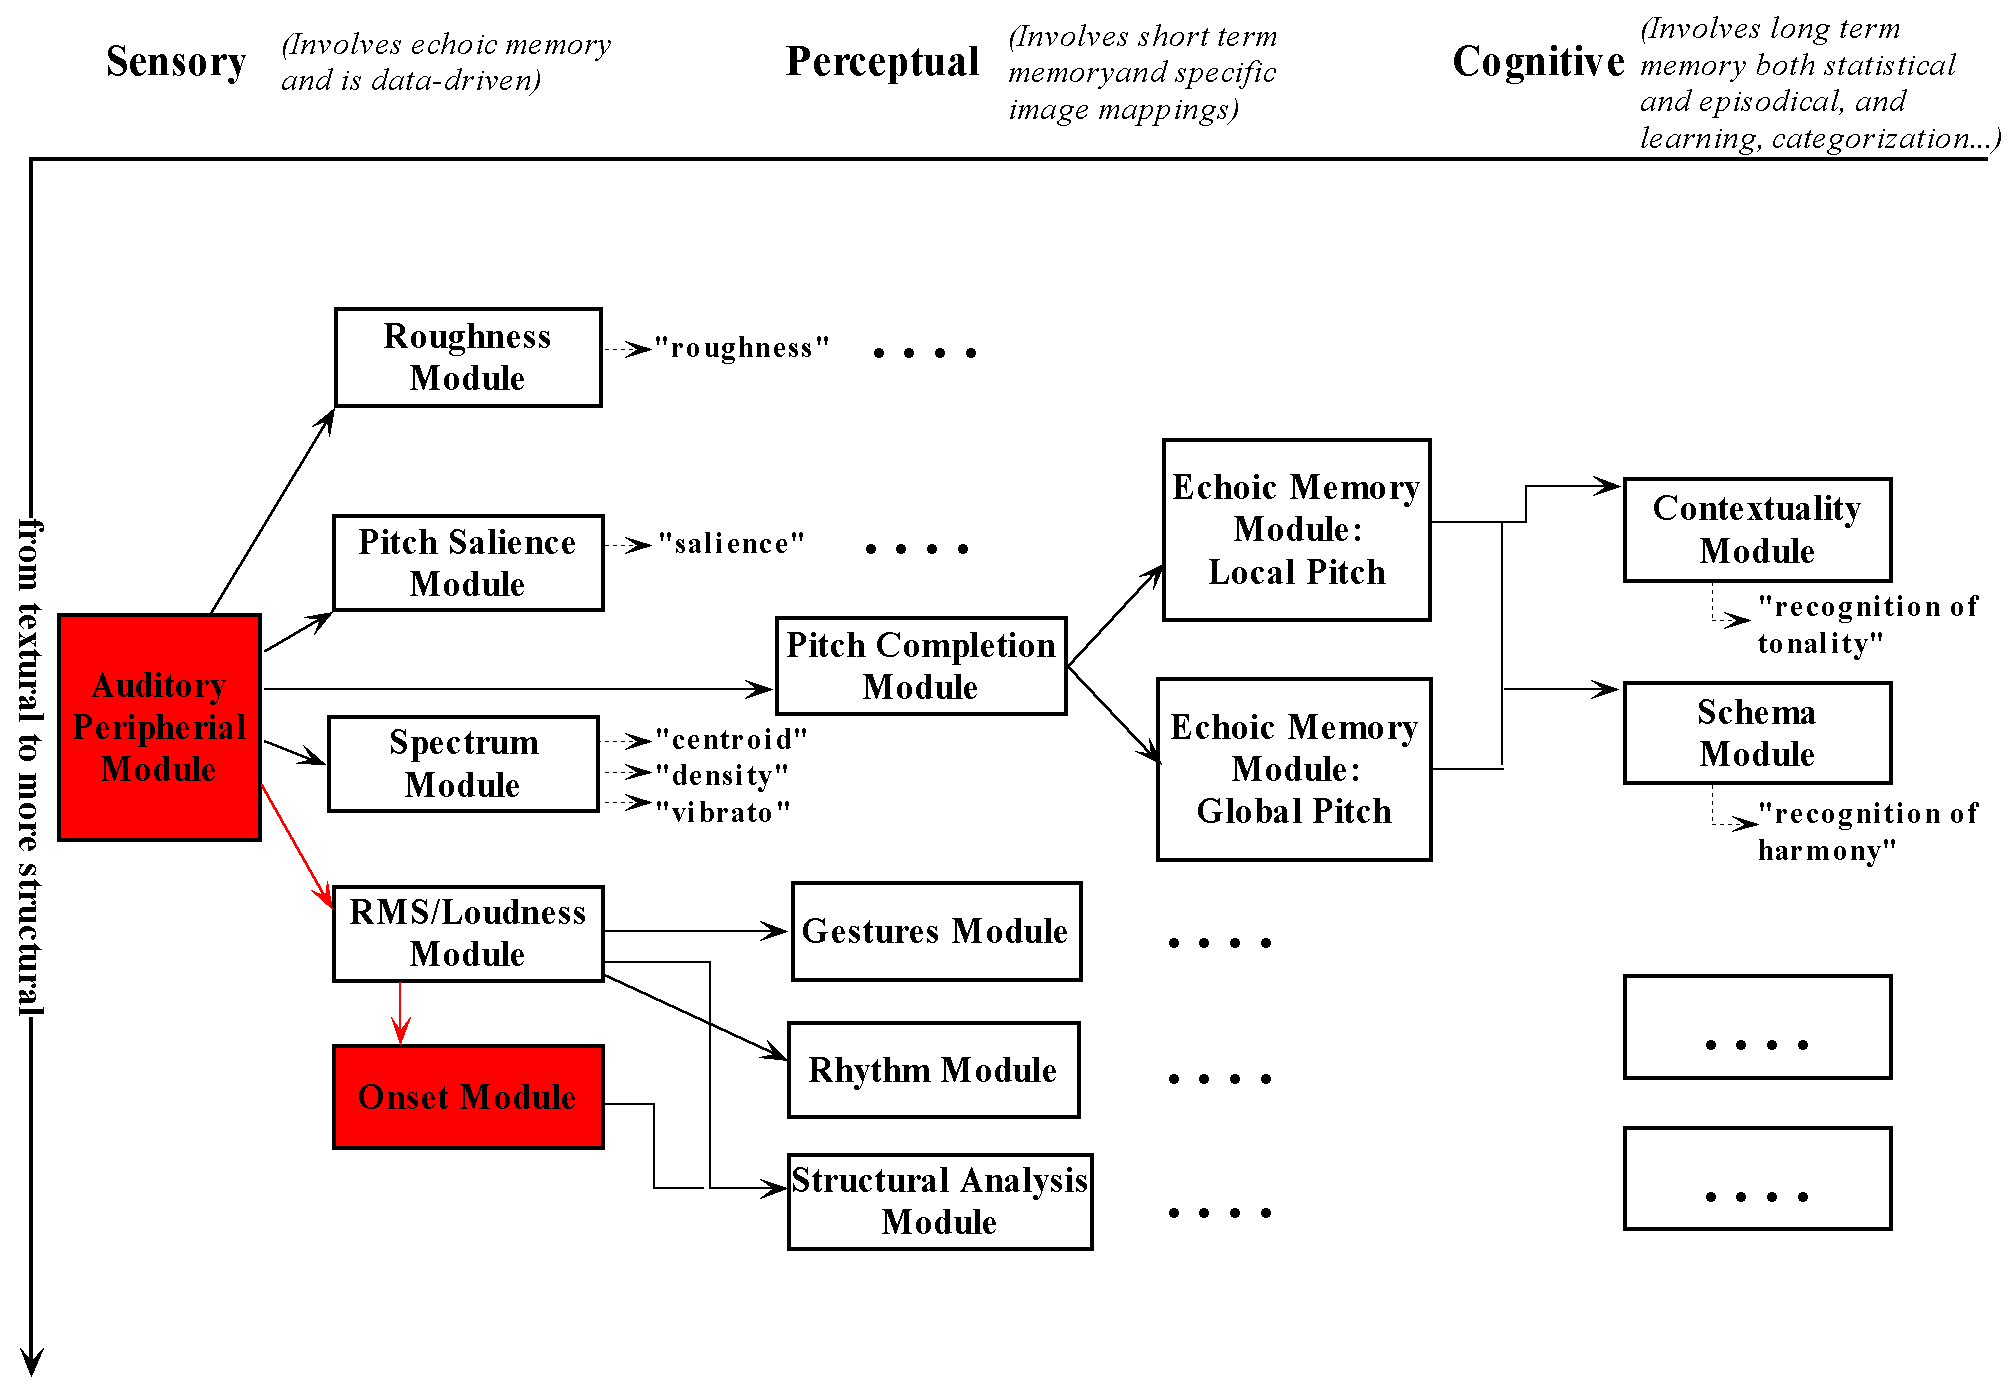
\includegraphics[width=\textwidth]{Graphics/ModulesOM}
    \caption{Chart of image transformation modules, with OM highlighted}
    \label{Fig:ModulesOM}
\end{figure}

The onset module analyzes the energy in the different auditory
channels. It extracts the relevant peaks and combines the results
for each channel to an overall onset estimation. Keep in mind that
onset detection is a rather difficult enterprise due to the fact
that some music instruments (violin, human voice, ...) have
gliding onsets which are hard to detect. Our onset module can be
used to chunk the frame-based representation into an event-based
representation. Figure \ref{Fig:OMModule} shows the modules
involved in the transformation process.
\begin{figure}[h]
    \centering
    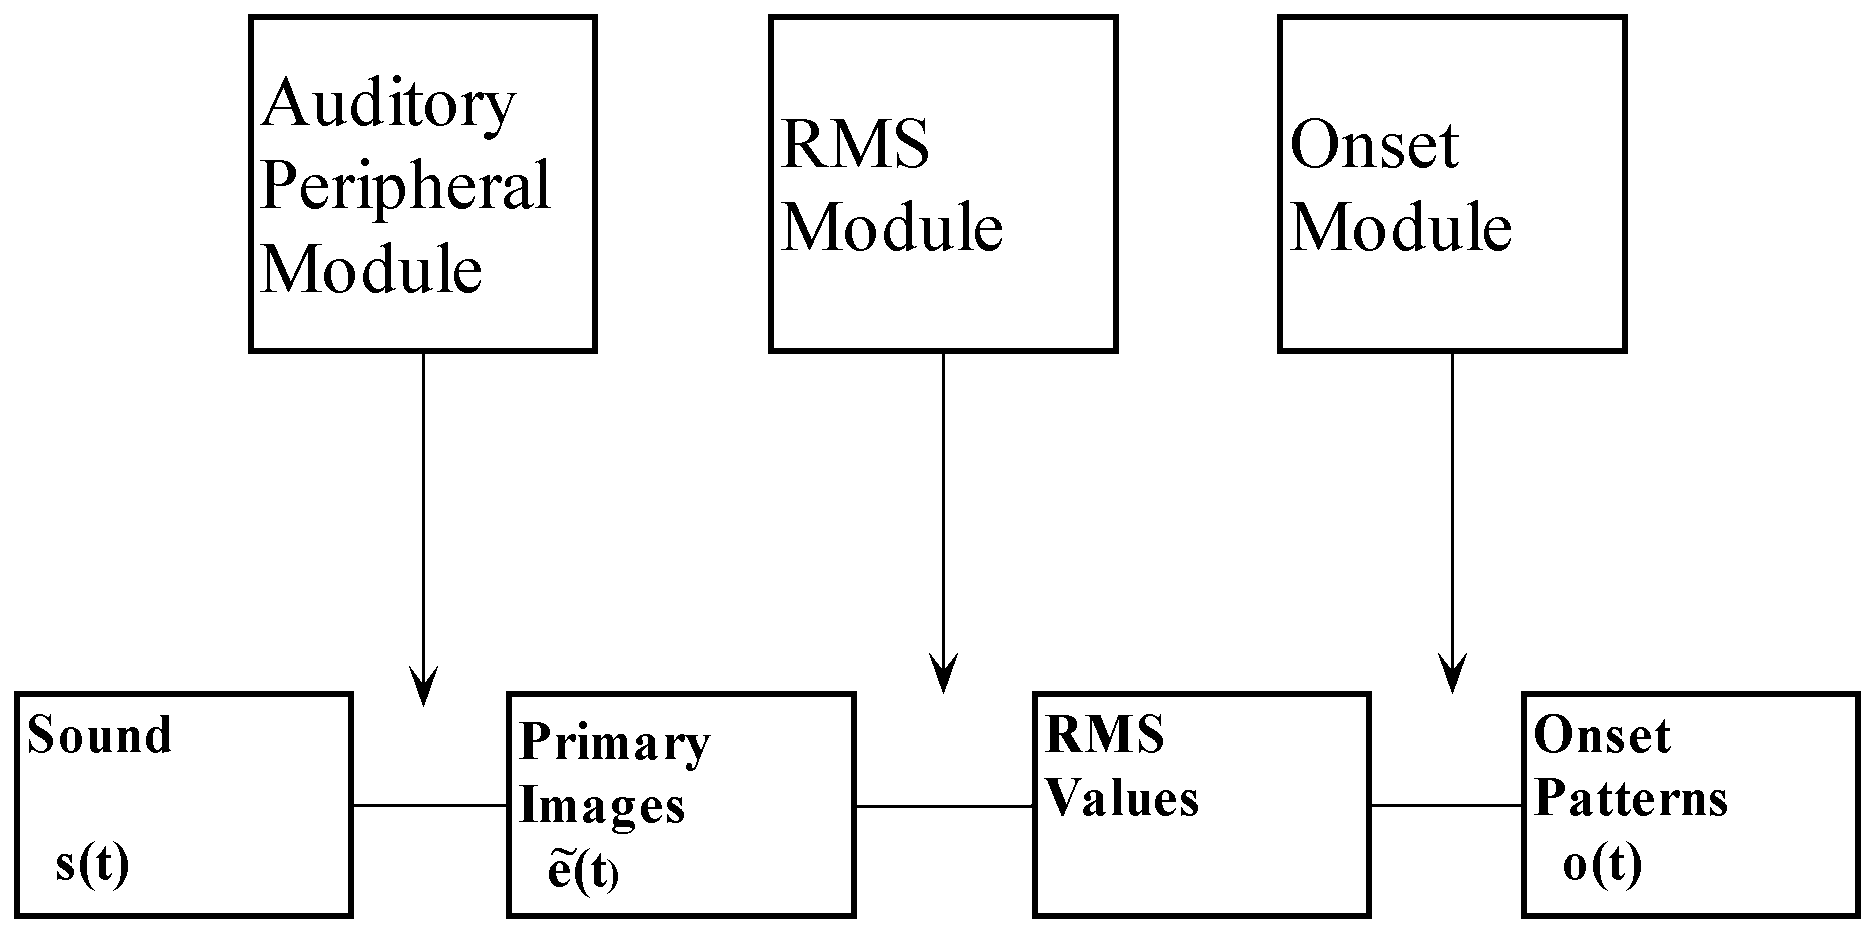
\includegraphics[width=\IPEMDefaultFigureWidth]{Graphics/OMModule}
    \caption{Modules involved for onset estimation.}
    \label{Fig:OMModule}
\end{figure}

\subsection{Functional-logical description}
% --------------------------------------------------------------------------------

The onset module involves:
\[APM: s(t) \rightarrow \tilde{e}(t)\]
\[RMS: \tilde{e}(t) \rightarrow \widetilde{rms}(t)\]
\[OM: \widetilde{rms}(t) \rightarrow o(t)\]
where APM provides the auditory nerve images and OM transforms
these images into the signal $o(t)$. A non-zero value in $o(t)$
corresponds to an onset at that moment, the value itself being
proportional to the estimated relevance of the onset.

\subsection{Signal processing description}
% --------------------------------------------------------------------------------

The algorithm used for detection of onsets consists of the
following steps:
\begin{enumerate}
\item Calculation of auditory nerve image.\\
    The auditory nerve image is calculated
    using the \hyperlink{Concepts:AuditoryPeripheralModule}{Auditory Peripheral Module}.
\item Calculation of RMS.\\
    For each of the channels in the ANI, the root mean square values are calculated using
    a frame size of 0.029 s and a frame step of 0.0058 s.
    For each frame $F$ in each channel, an RMS value is calculated according to:
    \begin{displaymath}
    RMS = \sqrt{\frac{\displaystyle \sum_{i=1}^{N}{F_{i}^2}}{N}}
    \end{displaymath}
    where $N$ = frame width in samples, and $F_{i}$ is the i-th sample of frame
    $F$.
    There is a toolbox function for the calculation of RMS values,
    see \hyperlink{FuncRef:IPEMCalcRMS}{IPEMCalcRMS}.
\item Low pass filtering.\\
    Each of these RMS-averaged channels is filtered with a second-order low pass Butterworth filter
    with a cutoff frequency of 15 Hz. This is done to reduce small, irrelevant peaks in the RMS signal.
\item Peak detection.\\
    Detection of relevant peaks in each channel is the tricky
    part....
    We start with all true peaks: moments where the first derivative goes from positive to negative.
    Then, the following approach is used for deciding whether a peak in a channel should be kept as an
    onset candidate for that channel:
    \begin{itemize}
    \item ignore everything below a certain threshold
    \item only keep peaks that are significantly bigger than their neighbors
    \item apply a mask so that following peaks due to irrelevant vibrations are thrown out
    \item for all remaining peaks, keep the biggest ones within a certain neighborhood, but only
          if it's big enough compared to the median value at that point
    \end{itemize}
\item Application of integrate-and-fire neural network.\\
    The contribution of this part is to cluster the peaks detected in the previous step over
    all channels and over time.
    This algorithm is based on an article by \citeA{Smith:1996}.
    One integrate-and-fire neuron is used per channel.
    Each neuron receives input from a set of
    adjacent channels, accumulates its input over time
    and its output is fed back to a number
    of adjacent neurons.
    The neuron dynamics are given by:
    \begin{displaymath}
    \frac{dA}{dt} = I(t) - diss\times{A} \qquad \textrm{with:
        \begin{tabular}[t]{l}
            $A$ = neurons' accumulated value \\
            $I$ = input \\
            $diss$ = dissipation factor
        \end{tabular}
        }
    \end{displaymath}

    If a neurons' accumulated value exceeds a certain threshold, it fires and the accumulated value
    is reset to zero. After firing, the neuron becomes insensitive to input for some period,
    called the refractory period. This configuration produces a sharp bursts of spikes when a
    number of channels provide evidence for onsets.
\item Final filtering.\\
    The onset pattern is finally filtered using the following approach:
    an onset is detected at a certain moment\\
    \begin{tabular}[t]{l}
        - if a certain number of channels detected an onset within
        a specific period of time, and\\
        - if the moment falls at least a minimum period of time
        behind the last detected onset\\
    \end{tabular}
\end{enumerate}

The result of these steps is a signal where a non-zero value
indicates the presence of an onset. To get an indication for the
relevance of a specific onset, we have used the number of
channels that detected an onset divided by the total number of
channels.

\subsection{Implementation}
% --------------------------------------------------------------------------------

\begin{tabularx}{\linewidth}{llX}
\hyperlink{FuncRef:IPEMCalcOnsets}{IPEMCalcOnsets} & - & Calculates onsets of sound signal\\
\hyperlink{FuncRef:IPEMCalcOnsetsFromANI}{IPEMCalcOnsetsFromANI} & - & Calculates onsets starting from an ANI\\
\hyperlink{FuncRef:IPEMDoOnsets}{IPEMDoOnsets} & - & Calculates onsets of sound file\\
\hyperlink{FuncRef:IPEMOnsetPattern}{IPEMOnsetPattern} & - & Integrate-and-fire neural net for onset detection\\
\hyperlink{FuncRef:IPEMOnsetPatternFilter}{IPEMOnsetPatternFilter} & - & Filters onset detection peak pattern\\
\hyperlink{FuncRef:IPEMOnsetPeakDetection}{IPEMOnsetPeakDetection} & - & Detects possible onset peaks in multi-channel signal\\
\hyperlink{FuncRef:IPEMOnsetPeakDetection1Channel}{IPEMOnsetPeakDetection1Channel} & - & Detects possible onset peaks in single channel\\
\hyperlink{FuncRef:IPEMSnipSoundFileAtOnsets}{IPEMSnipSoundFileAtOnsets} & - & Cuts sound file in segments at onsets\\
\end{tabularx}


\subsection{Examples}
% --------------------------------------------------------------------------------

To extract the onsets from
\IPEMSound{Sounds/SchumannKurioseGeschichte.wav}{Schumann's
Kuriose Geschichte}, use the following expression:\\

\begin{IPEMCodeEnvironment}
[Ts,Tsmp] = IPEMDoOnsets('SchumannKurioseGeschichte.wav');
\end{IPEMCodeEnvironment}\\

You can of course split the module in the several subparts. For
example, if you first process the file with the Auditory
Peripheral Module, and then apply the onsets module, you could
use:\\

\begin{IPEMCodeEnvironment}
[ANI,ANIFreq,ANIFilterFreqs] = IPEMCalcANIFromFile('SchumannKurioseGeschichte.wav');
\newline [OnsetSignal,OnsetFreq] = IPEMCalcOnsetsFromANI(ANI,ANIFreq);
\end{IPEMCodeEnvironment}\\

Figures \ref{Fig:OnsetsANIAndRMS} to \ref{Fig:OnsetsSegmentation}
illustrate the different steps for this particular example.

\begin{figure}[h]
    \centering
    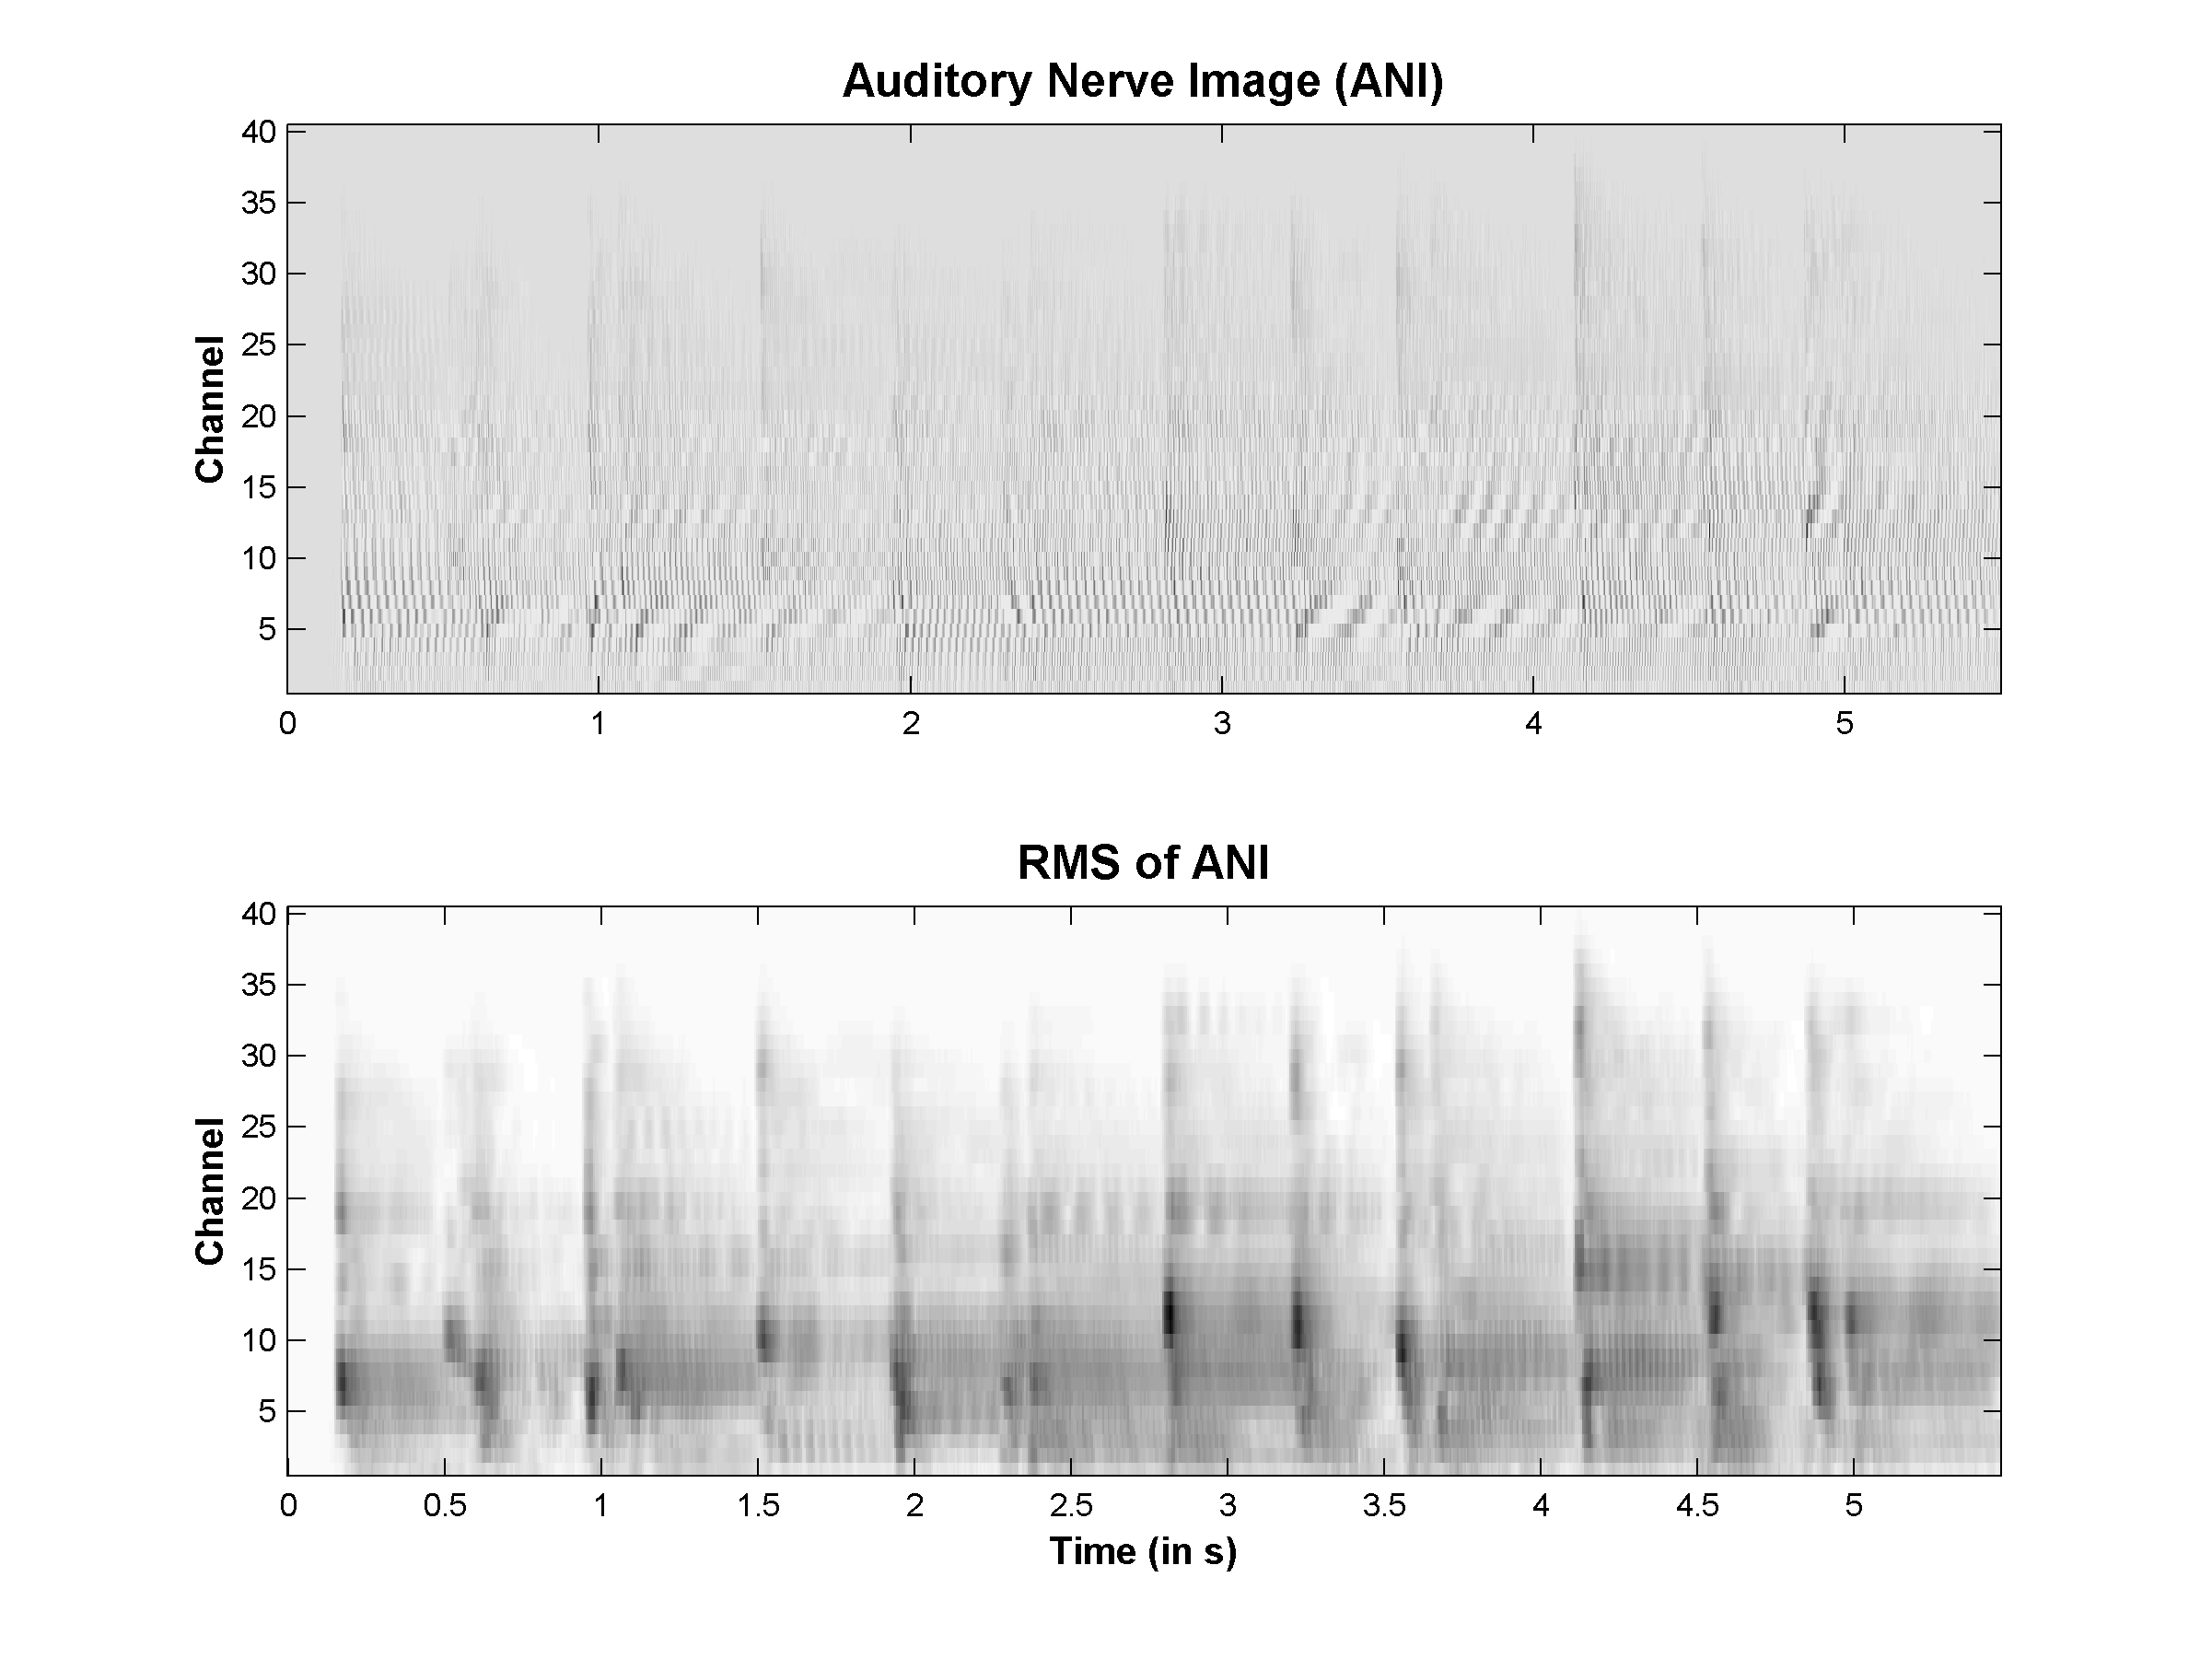
\includegraphics[width=\IPEMDefaultFigureWidth]{Graphics/OnsetsANIAndRMS}
    \caption{Top: ANI of the Schumann sound excerpt. Bottom: RMS values of the ANI.}
    \label{Fig:OnsetsANIAndRMS}
\end{figure}

\begin{figure}[h]
    \centering
    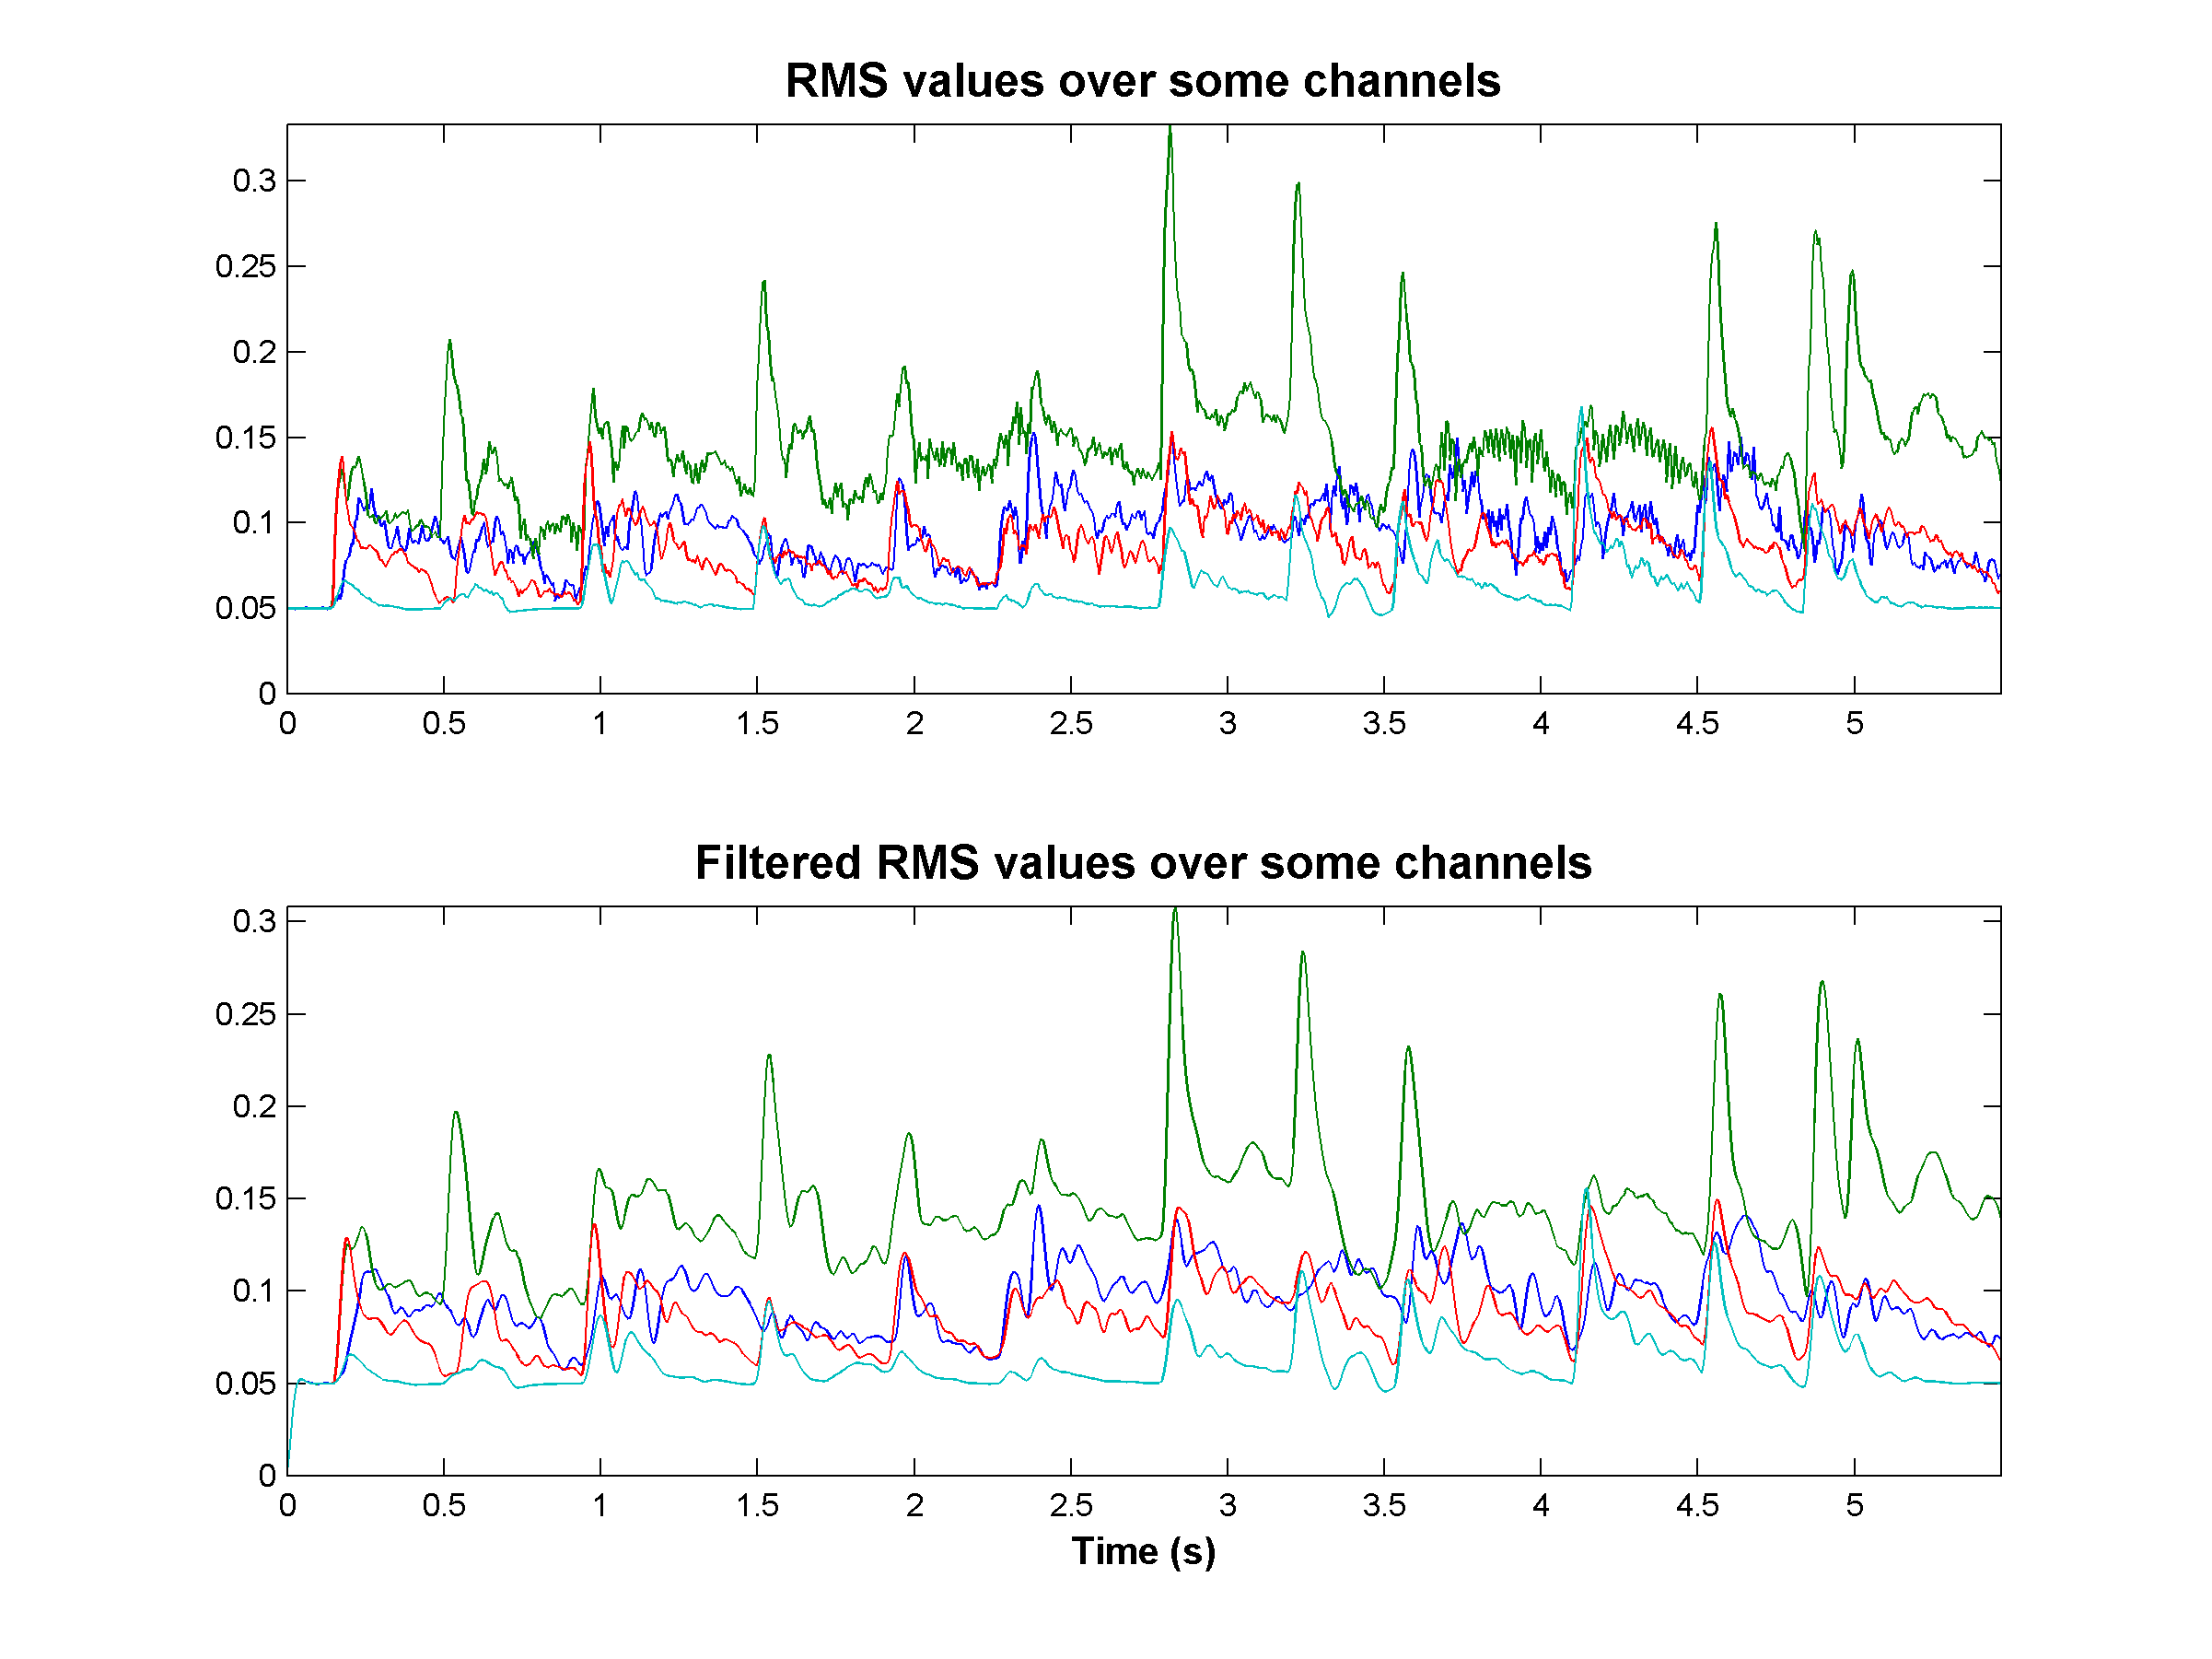
\includegraphics[width=\IPEMDefaultFigureWidth]{Graphics/OnsetsFilteredRMS}
    \caption{Top: RMS values for some channels of the ANI. Bottom: low pass filtered RMS values for the same channels.}
    \label{Fig:OnsetsFilteredRMS}
\end{figure}

\begin{figure}[h]
    \centering
    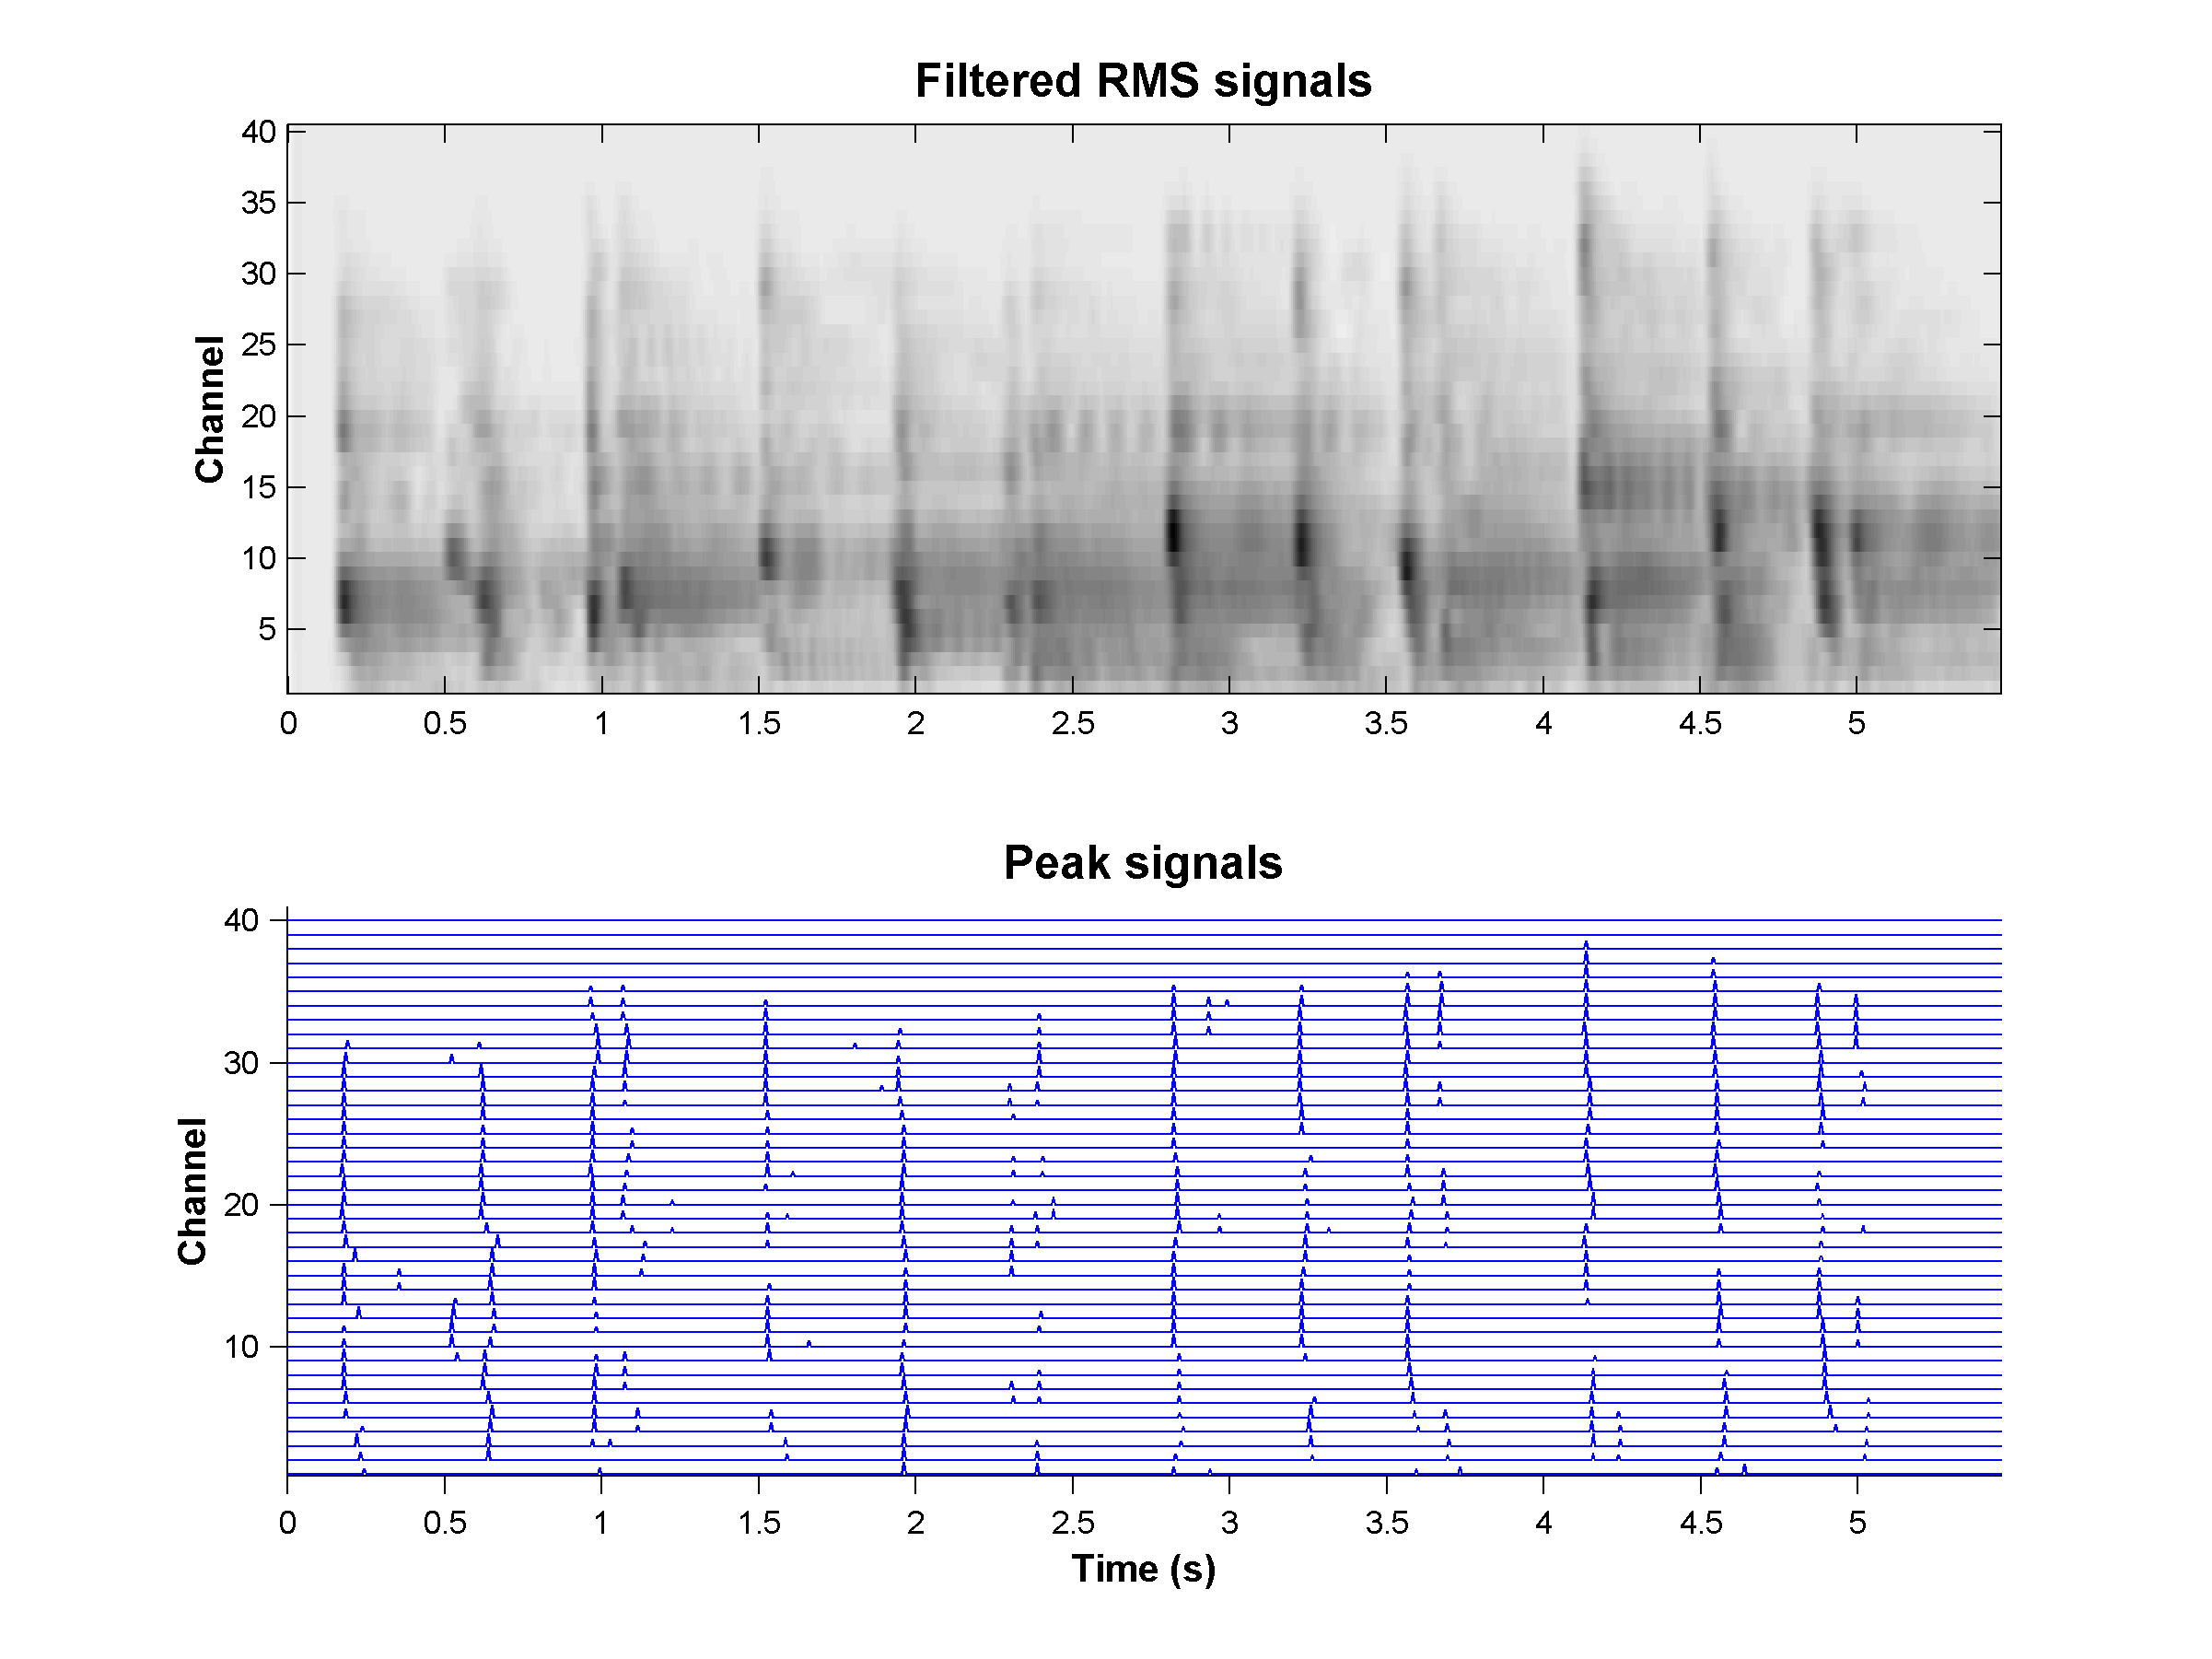
\includegraphics[width=\IPEMDefaultFigureWidth]{Graphics/OnsetsOnsetPeakDetection}
    \caption{Top: filtered RMS values of the ANI. Bottom: peaks detected for each channel.}
    \label{Fig:OnsetsOnsetPeakDetection}
\end{figure}

\begin{figure}[h]
    \centering
    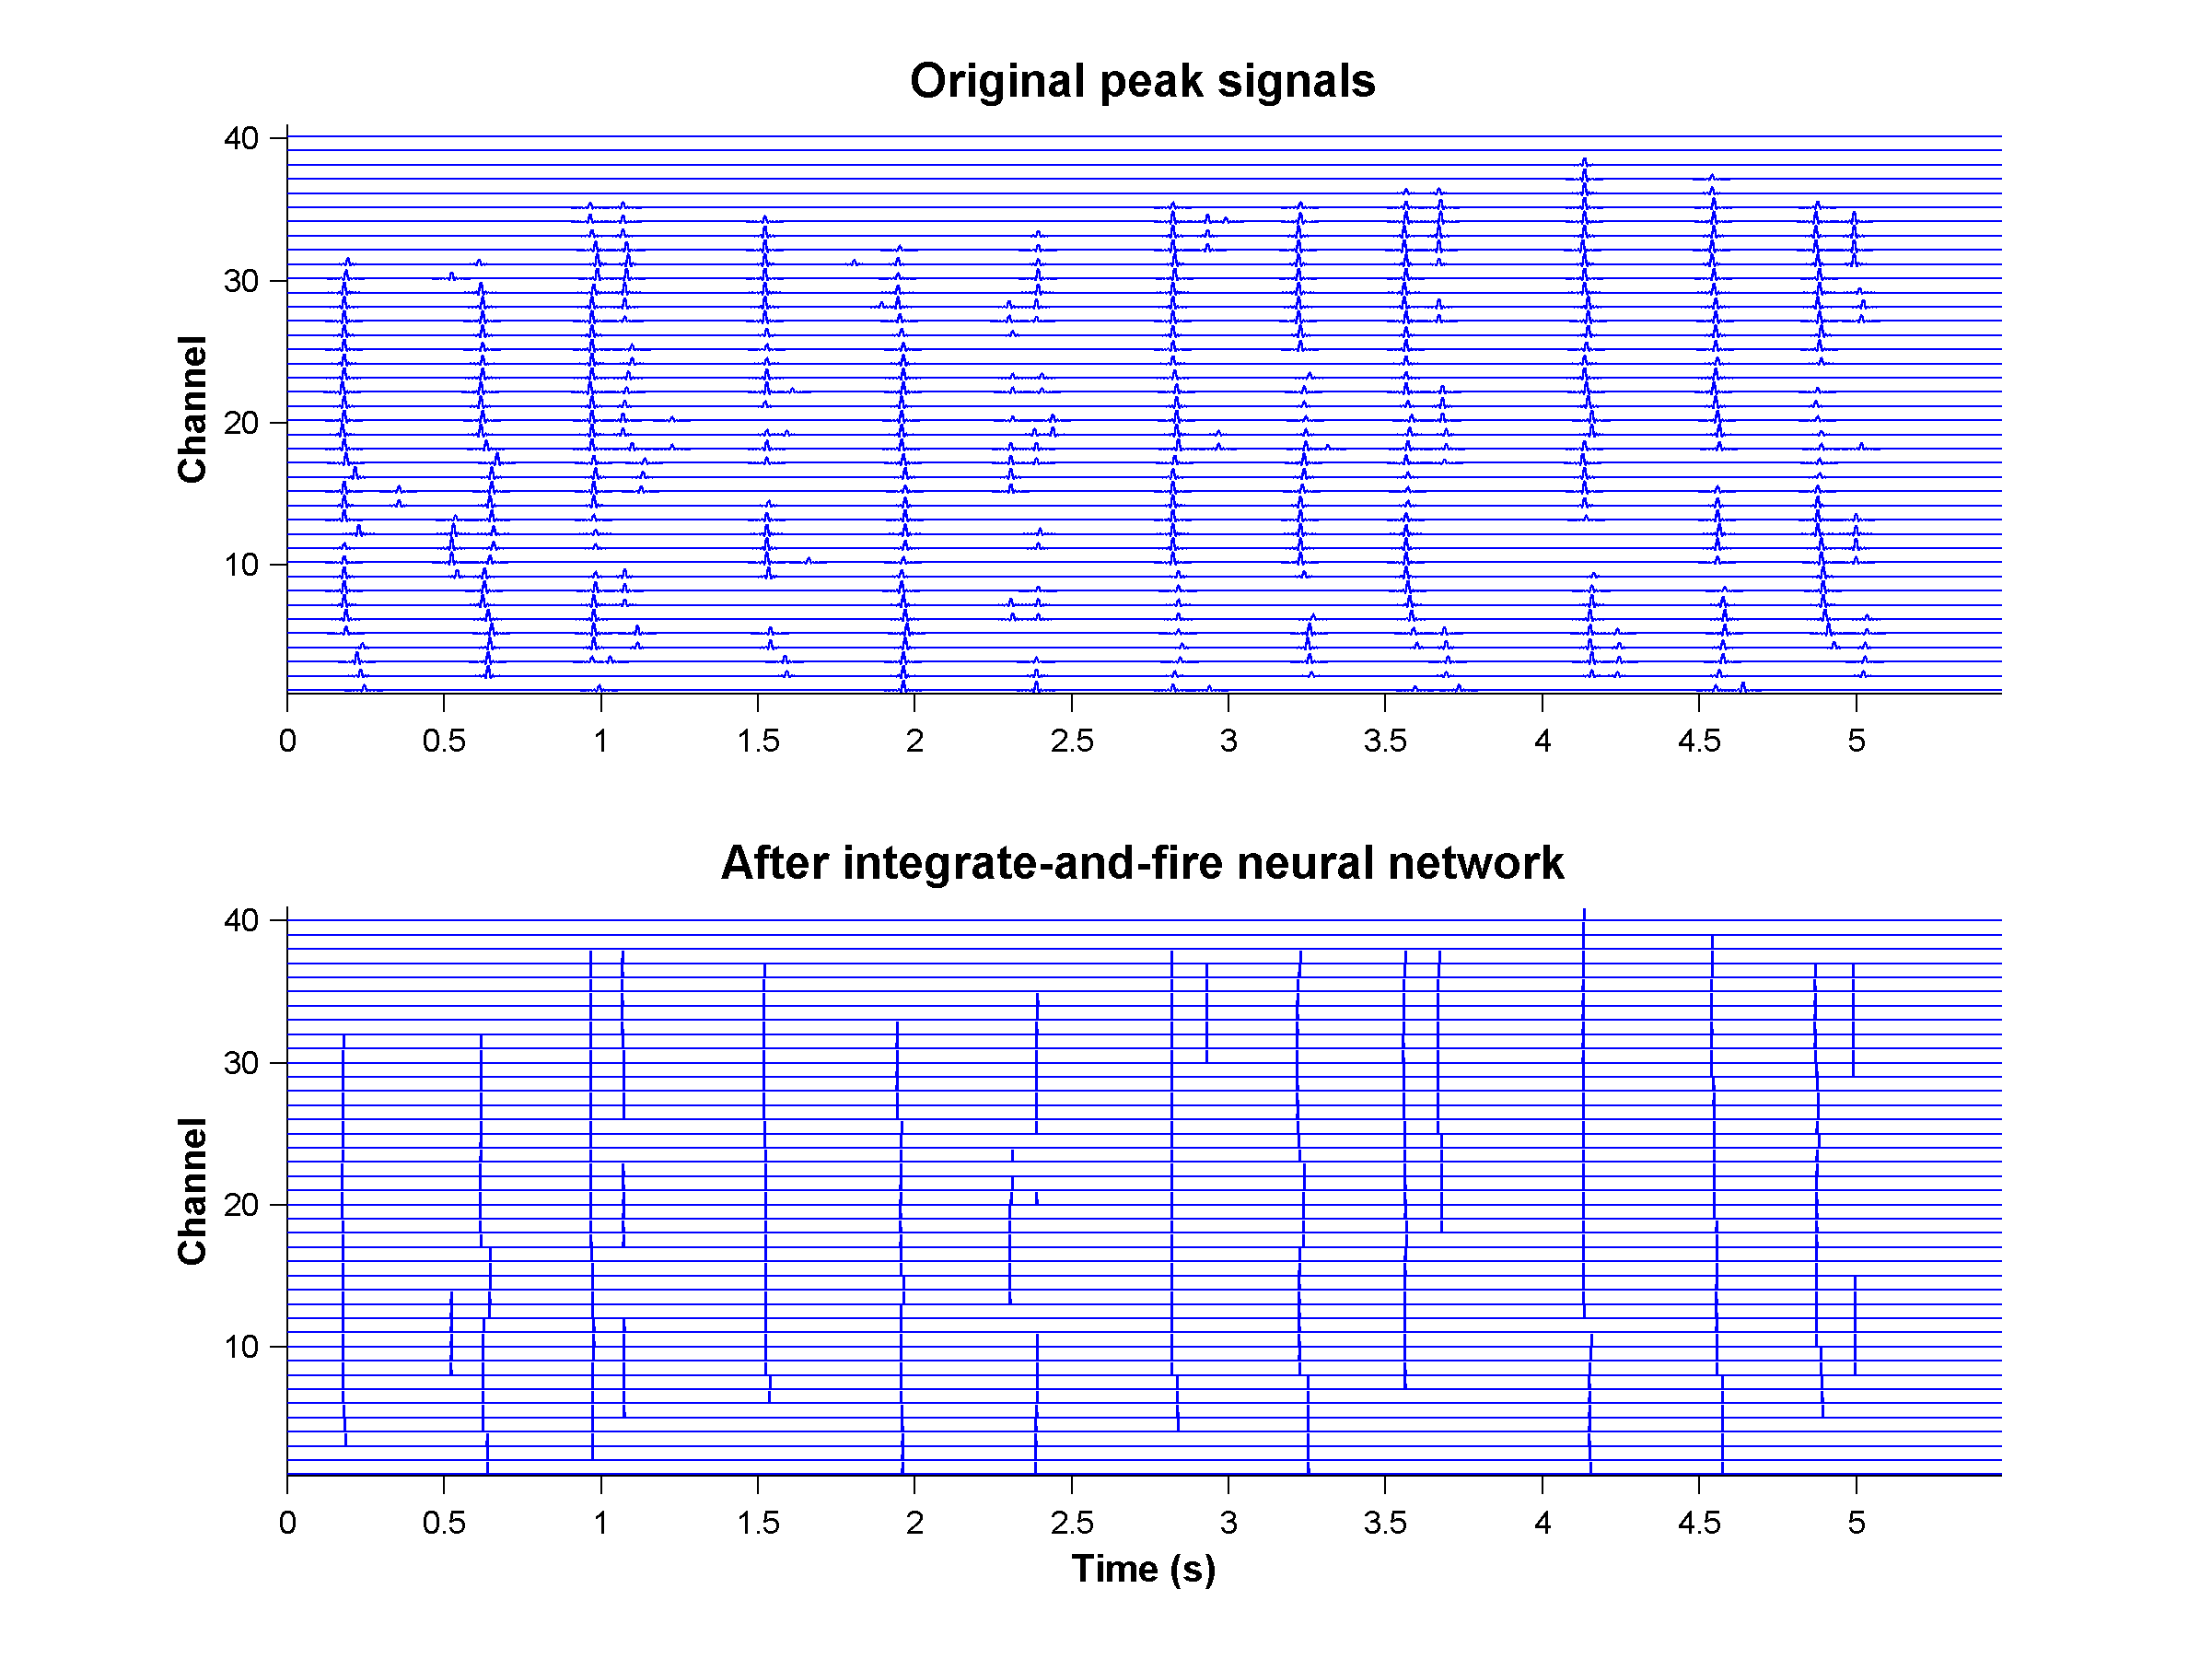
\includegraphics[width=\IPEMDefaultFigureWidth]{Graphics/OnsetsOnsetPattern}
    \caption{Top: detected peaks. Bottom: peaks after applying the integrate-and-fire neural network.}
    \label{Fig:OnsetsOnsetPattern}
\end{figure}

\begin{figure}[h]
    \centering
    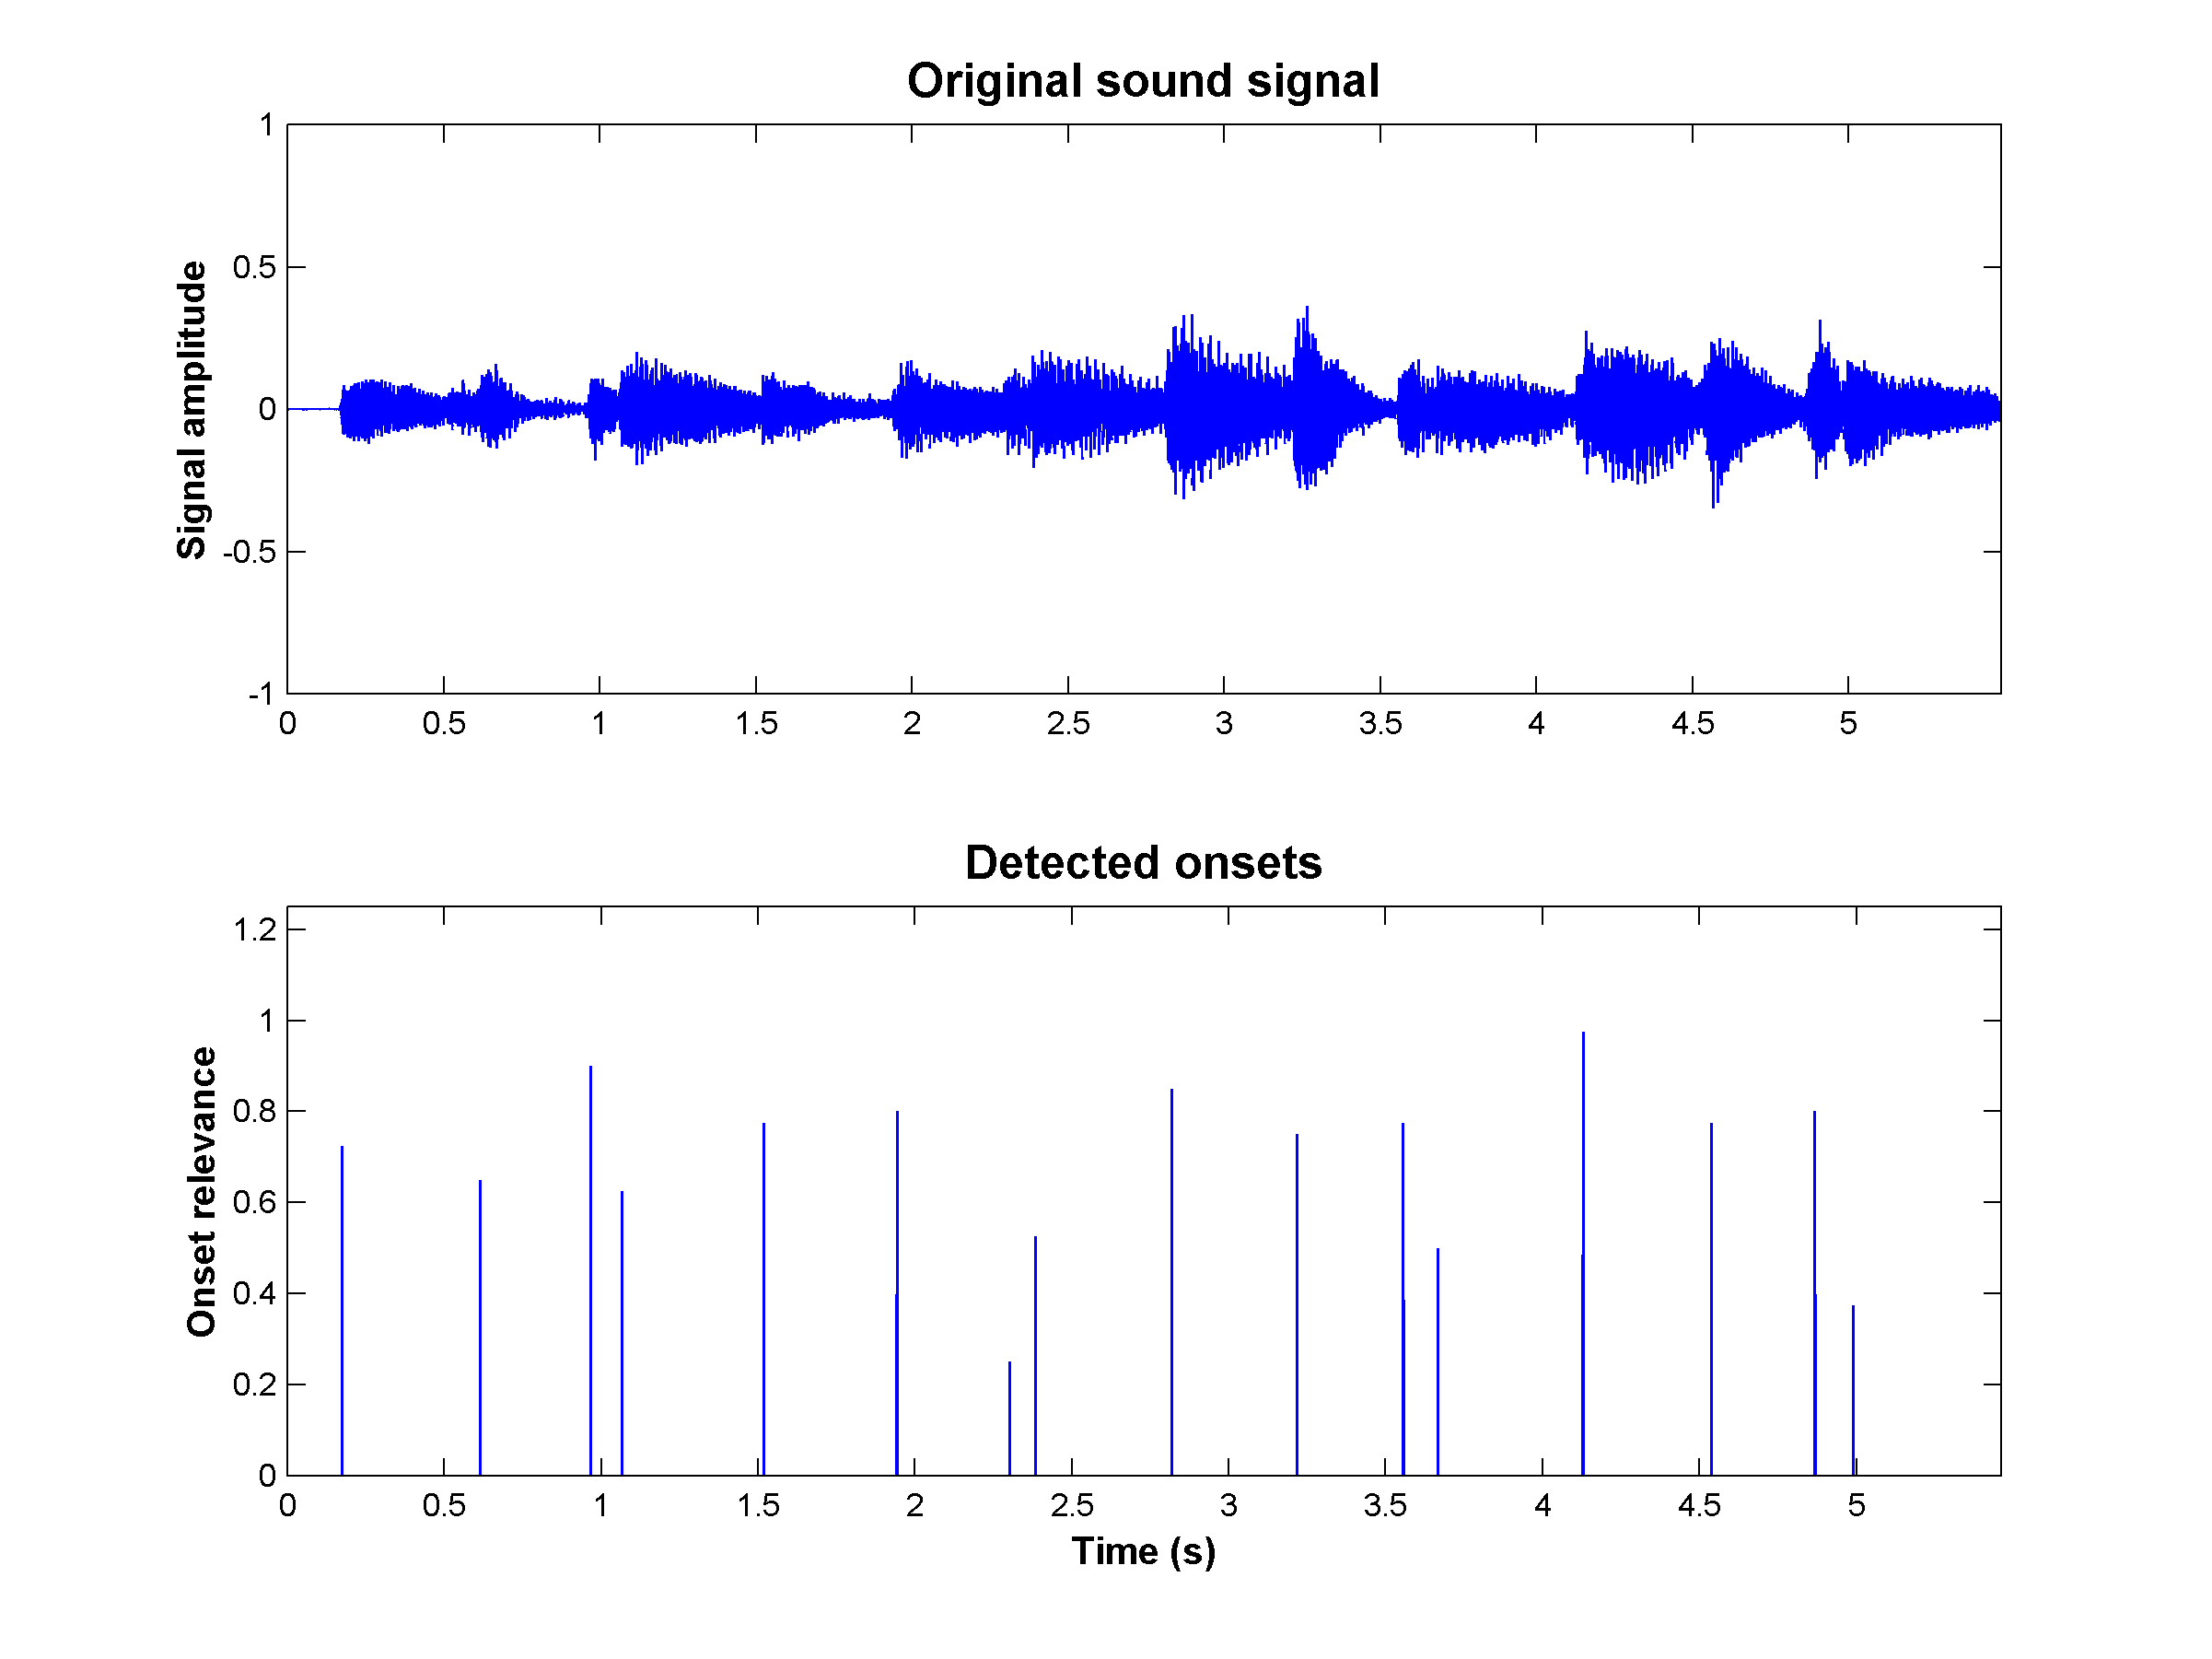
\includegraphics[width=\IPEMDefaultFigureWidth]{Graphics/OnsetsOnsetFilter}
    \caption{Top: original sound signal. Bottom: detected onsets and their relevance level.}
    \label{Fig:OnsetsOnsetFilter}
\end{figure}

\begin{figure}[h]
    \centering
    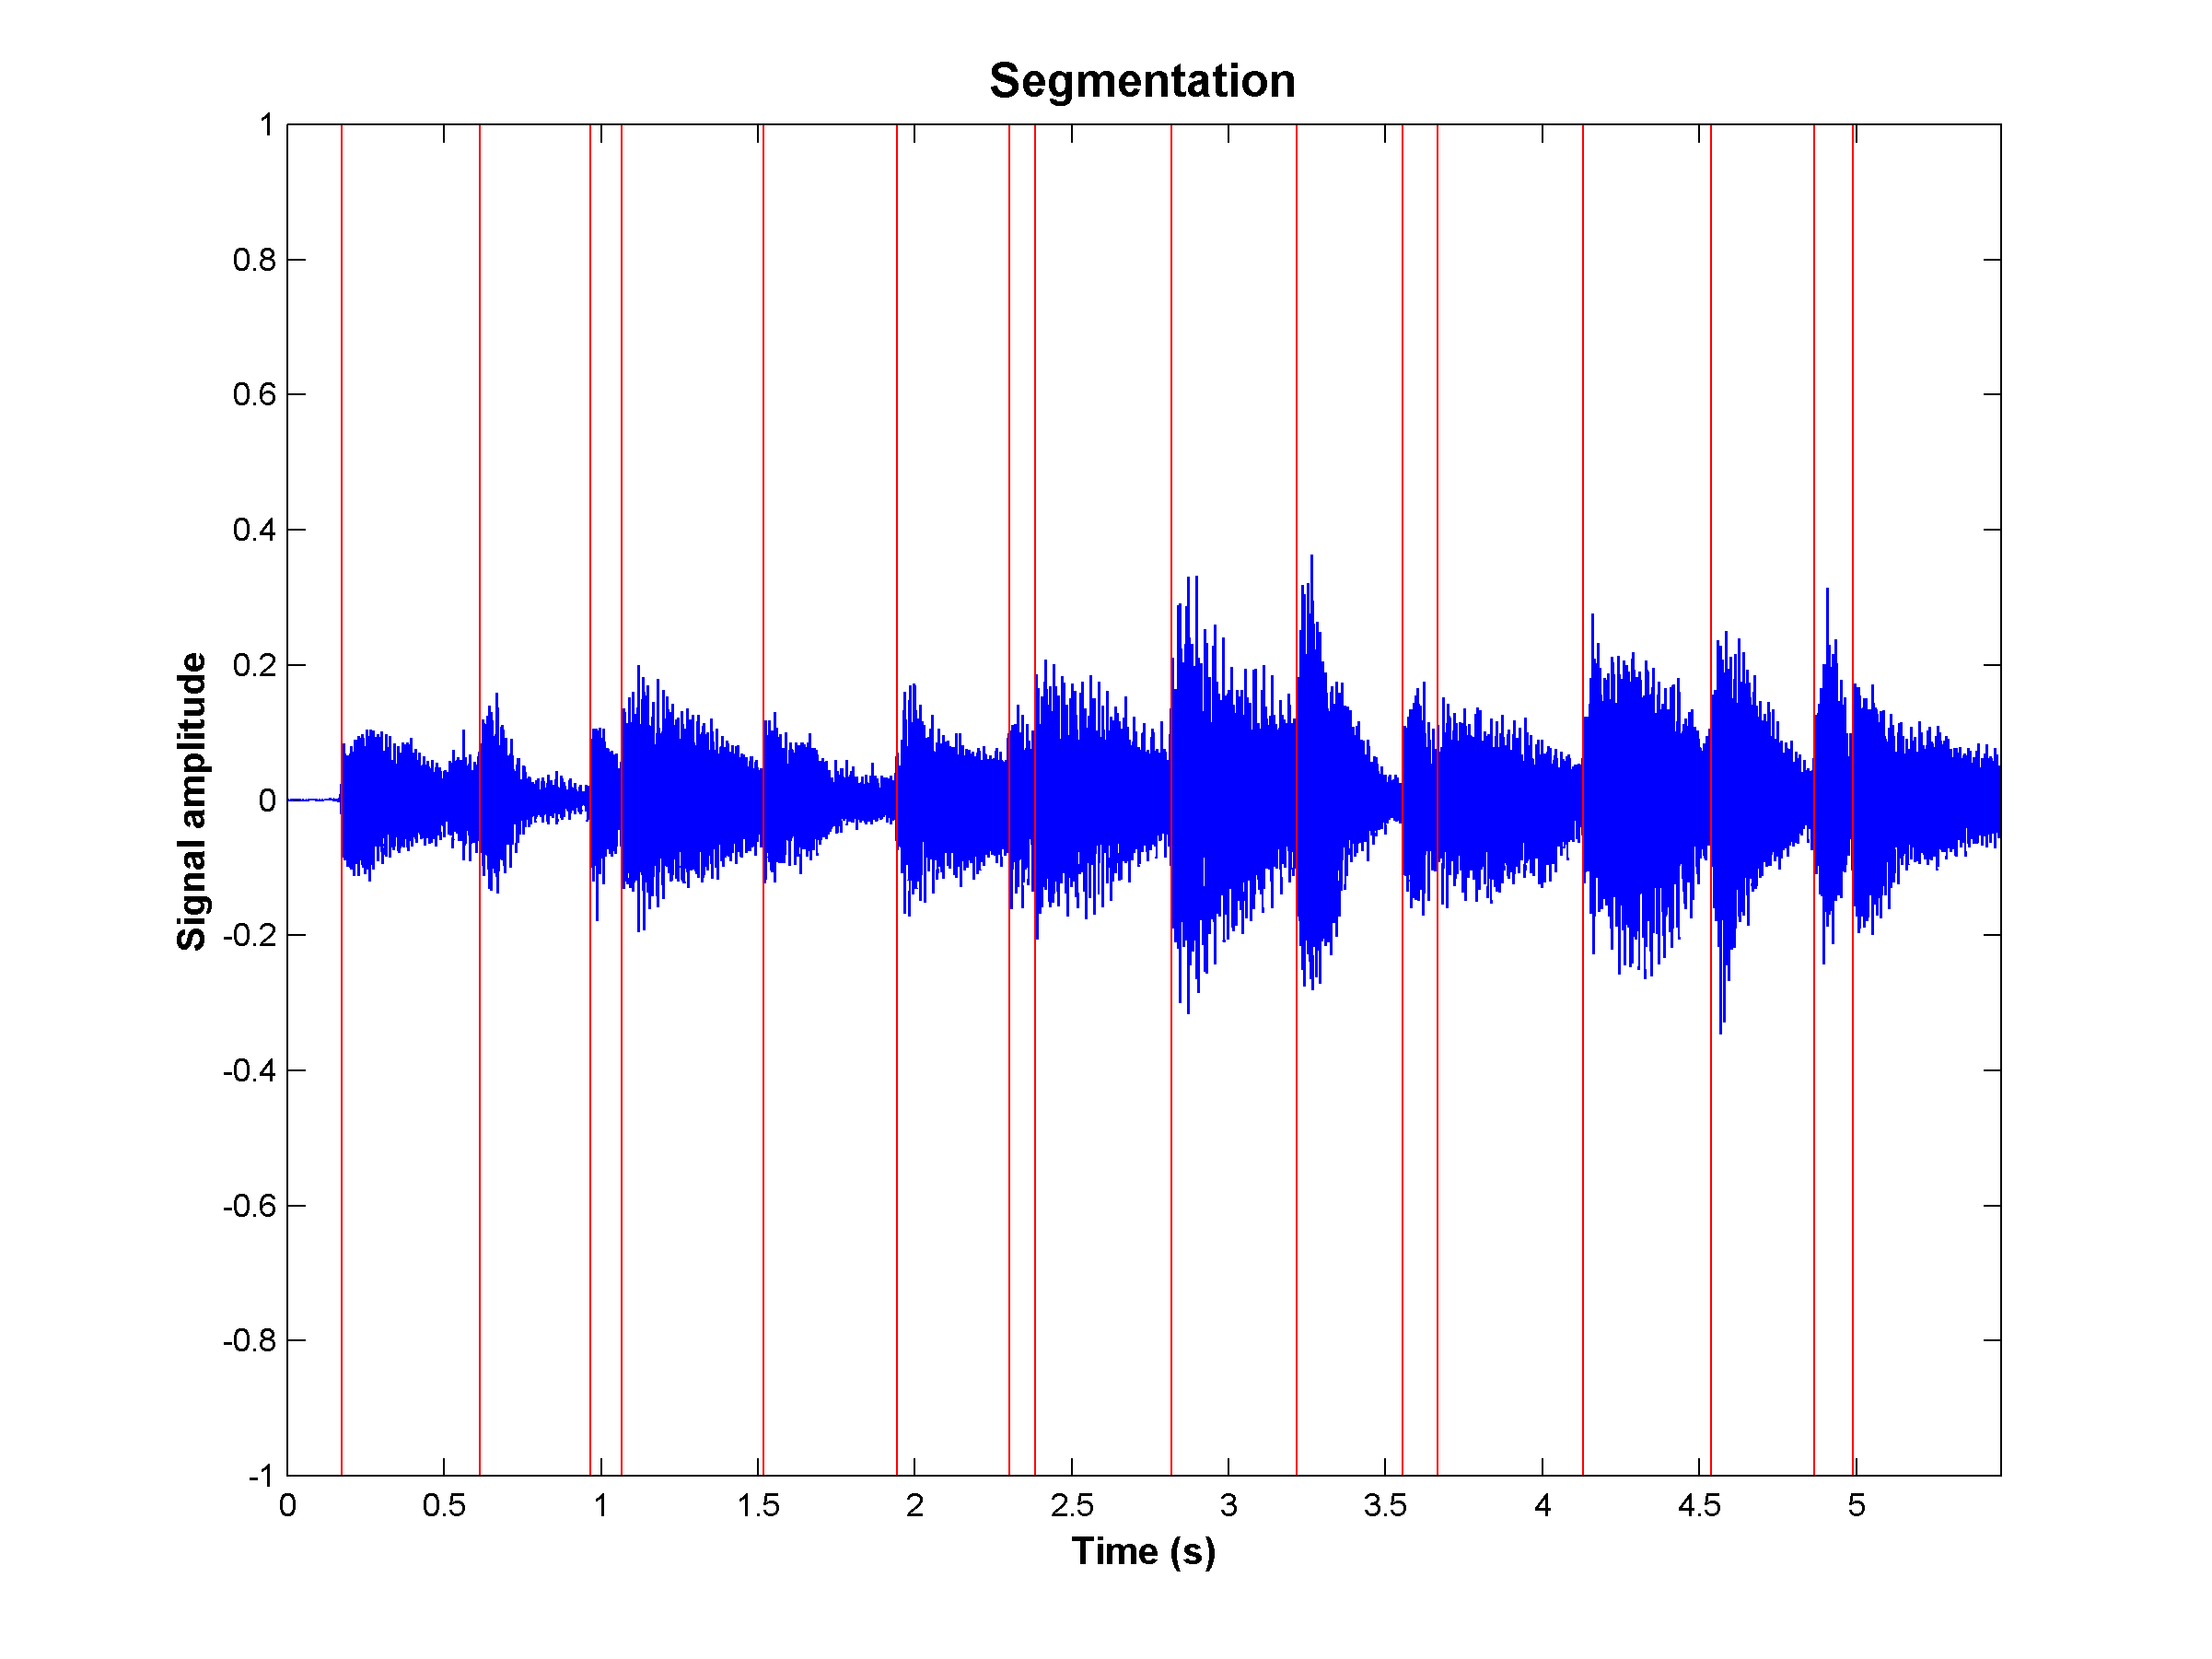
\includegraphics[width=\IPEMDefaultFigureWidth]{Graphics/OnsetsSegmentation}
    \caption{Segmentation of the original sound signal using the onset module.}
    \label{Fig:OnsetsSegmentation}
\end{figure}

% --------------------------------------------------------------------------------

% --------------------------------------------------------------------------------
% --------------------------------------------------------------------------------
\newpage
\section{Pitch Completion Module}
% --------------------------------------------------------------------------------

% Make general target
\hypertarget{Concepts:PitchCompletionModule}{}

% Make target for following functions:
\hypertarget{Concepts:IPEMPeriodicityPitch}{}

\subsection{Introductory description}
% --------------------------------------------------------------------------------

The Pitch Completion Module (PCM) calculates the periodicity pitch
image of a signal. Strictly speaking, the neural rate code of the
auditory nerve images is taken as input and a periodicity analysis
is the output. Otherwise stated, the inputs are primary images and
the outputs are pitch images. In our global chart of image
transformation modules PCM is localized in the section on
perception (fig. \ref{Fig:ModulesPCM}).
\begin{figure}[h]
    \centering
    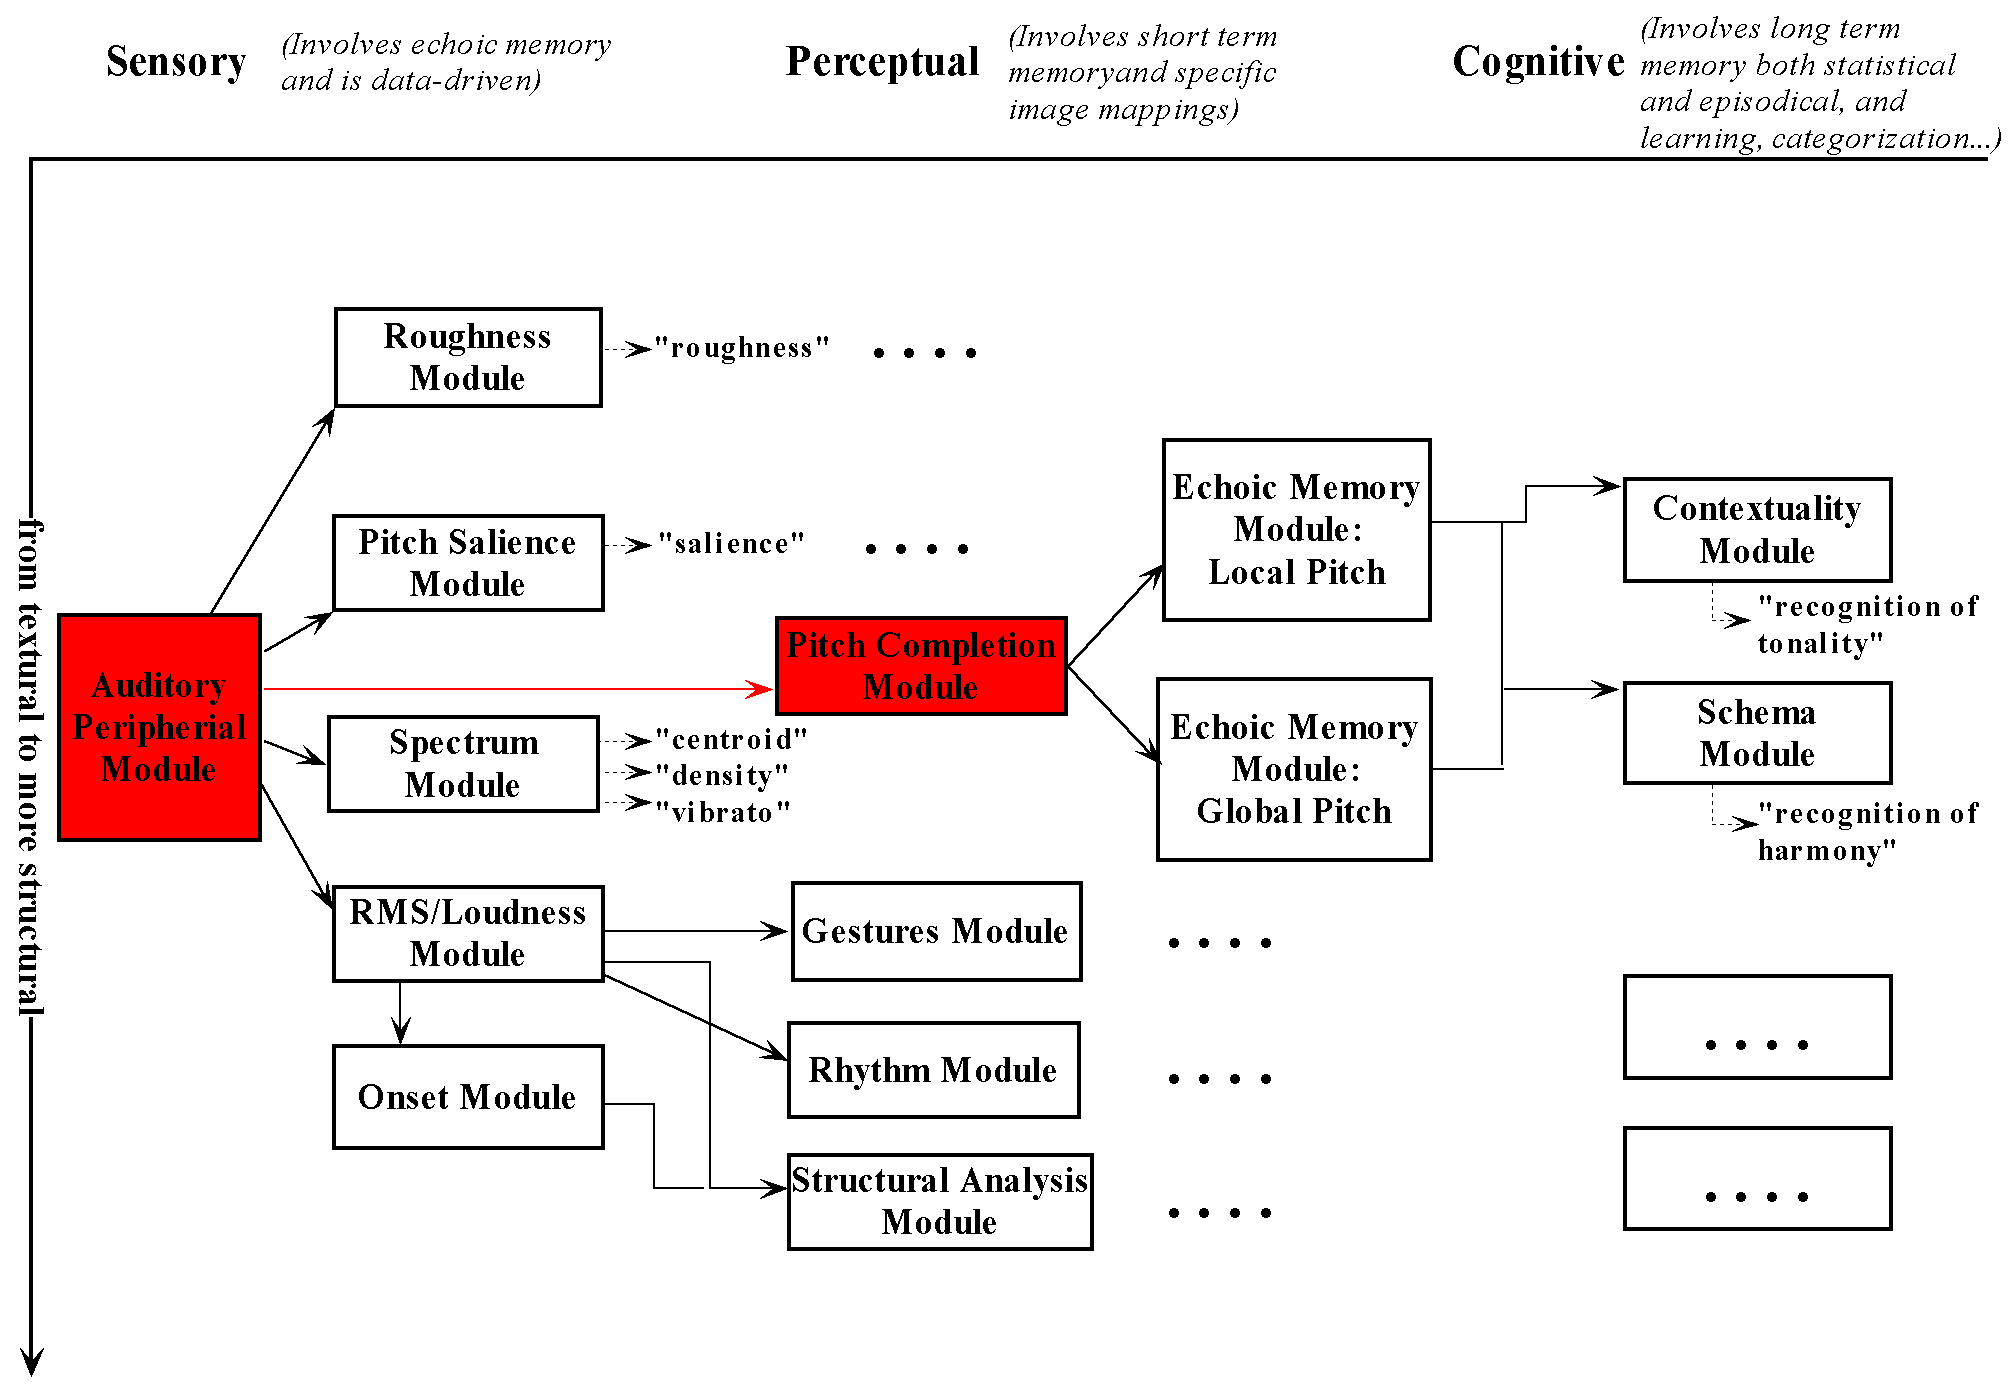
\includegraphics[width=\textwidth]{Graphics/ModulesPCM}
    \caption{Chart of image transformation modules, with PCM highlighted}
    \label{Fig:ModulesPCM}
\end{figure}

A periodicity analysis of primary images is dealt with at
different occasions, such as in
\hyperlink{Concepts:RhythmModule}{rhythm}. The main difference is
the focus of attention. In rhythm periodicity we look at larger
periodicities than in pitch where the focus of our attention is
between 80 and 1250 Hz.
\begin{itemize}
\item
    The lower limit of 80 Hz accounts for the fact that for smaller frequencies,
    the sensation of pitch becomes more a sensation of textural properties.
    This is a shift of perceptual categorization which is taken into account
    in our modeling. Indeed, our model of \hyperlink{Concepts:RoughnessModule}{roughness}
    took into account a range of frequencies between 5 and 300 Hz but
    the focus was on frequencies between 50 and 70 Hz (see the filter characteristics
    in figure \ref{Fig:Filters}).
\item
    The higher limit of 1250 Hz is related to the limits of neural synchronization.
    Beyond about 1250 Hz, the neurons are no longer able to follow the exact
    period of the signal very accurately, and periodicity pitch becomes unreliable.
\end{itemize}
Pitch estimations at higher frequencies could rely on spectral
information contained in $e(t,c)$. Such spectral images could be
obtained by taking the RMS-values in each channel over short time
periods using \hyperlink{FuncRef:IPEMCalcRMS}{IPEMCalcRMS}.
However, the pitch information necessary to deal with harmonic
relationships, is here assumed to be contained in the time-code of
the auditory nerve images, and this within a frequency band of 80
to 1250 Hz.

From a conceptual point of view the Pitch Completion Module
performs a transformation from time-code to place-code, i.e. from
patterns whose frequency is contained within the temporal
characteristics of the pattern to patterns whose frequency is
encoded along a spatial array. Physiological evidence for
periodicity pitch perception has been gathered by
\citeA{Langner:92,Langner:97}. Figure \ref{Fig:PCMModule} shows the
modules involved in the image transformation process.
\begin{figure}[h]
    \centering
    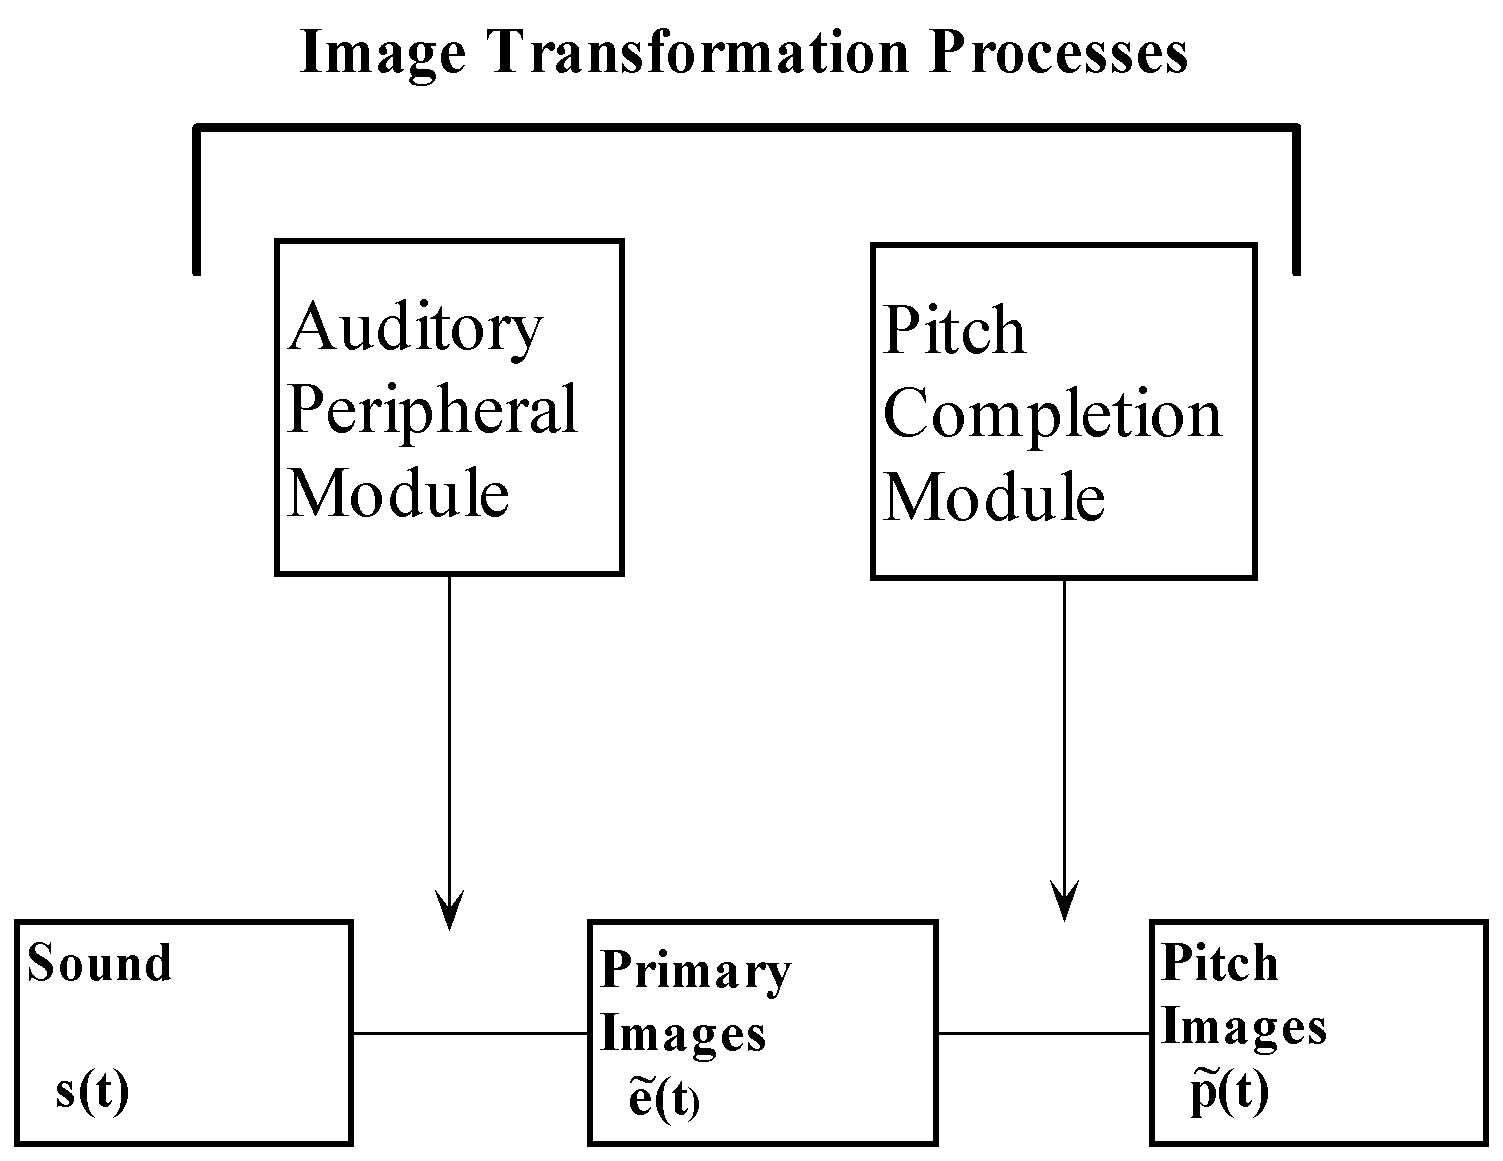
\includegraphics[width=\IPEMDefaultFigureWidth]{Graphics/PCMModule}
    \caption{Image Transformation Process: Pitch Completion Module}
    \label{Fig:PCMModule}
\end{figure}

\subsection{Functional-logical description}
% --------------------------------------------------------------------------------

First the auditory nerve images are calculated using the
\hyperlink{Concepts:AuditoryPeripheralModule}{Auditory Peripheral
Module}. The Pitch Completion Module then transforms these images
into pitch images.
\[APM:~ s(t) \rightarrow e(t,c)\]
\[PCM:~ e(t,c) \rightarrow p(t,\tau)~(=~\tilde{p}(t))\]

The Pitch Completion Module has two stages. First a periodicity
analysis of each $e(t,c)$ pattern, band-pass filtered for 80-1250
Hz, is made, where $f[e(t,c)]$ is the band-pass filtered auditory
nerve pattern for channel $c$, and $p(t,c,\tau)$ or
$\tilde{p}(t,c)$ the periodicity analysis of that pattern, with
$\tau$ denoting the period. The detected periods are registered
along a spatial array of periods. We thus have:
\begin{displaymath}
PCM1:~ \left[
\begin{array}{l}
f[e(t,1)] \\ f[e(t,2)] \\ \cdots \\ f[e(t,C)]
\end{array}
\right] \rightarrow \left[
\begin{array}{l}
\tilde{p}(t,1) \\ \tilde{p}(t,2) \\ \cdots \\ \tilde{p}(t,C)
\end{array}
\right]
\end{displaymath}

Secondly, a {\sl coincidence mechanism} sums up the
$\tilde{p}(t,c)$ over all channels patterns and stores the result
in a summary auto-correlation pattern called $\tilde{p}(t)$:
\begin{displaymath}
PCM2:~ \left[
\begin{array}{l}
\tilde{p}(t,1) \\ \tilde{p}(t,2) \\ \cdots \\ \tilde{p}(t,C)
\end{array}
\right] \rightarrow \tilde{p}(t)
\end{displaymath}

The resulting pattern $\tilde{p}$ (in alternative notation
$p(\tau)$) at time $t$ is called the pitch image or {\sl
completion image} at time $t$. The pitch is represented along the
$\tau$ axis. The completion image is related to the notion of
virtual pitch pattern. It gives an account of the common
periodicity along the auditory neurons in the frequency region of
80 Hz to 1250 Hz. Notice than the procedure outlined for PCM is
very similar to the procedure used for the detection of
periodicity in rhythm patterns, as described in the Example
section of the \hyperlink{Concepts:RhythmModule}{Rhythm Module}.

\subsection{Signal processing description}
% --------------------------------------------------------------------------------

These are the steps of the periodicity pitch calculation:

\begin{itemize}
\item Filtering\\
    The channels of the ANI are filtered between 80 and 1250 Hz. Due
    to the fact that the output of the auditory model gives the
    envelopes of the neural firing probabilities ($<$ 1250 Hz), it
    suffices to first apply a low-pass filter and then subtract that
    from the original signal in order to obtain the pitch. The
    low-pass filter is a second order Butterworth filter with a
    cutoff frequency of 80 Hz.
    \[ \tilde{e}_{filt}(t) = f[\tilde{e}(t)] \]
\item Auto-correlation\\
    A frame-based auto-correlation analysis is performed on the
    filtered channels. A frame width $FW$ and step size $FS$ are
    chosen and then for each frame and each channel $c$, we perform
    an auto-correlation for each time-lag $\delta$:
    \[
        p(t,c,\delta) = \int_{t}^{t+FW}{e_{filt,c}(\tau).e_{filt,c}(\tau+\delta).d\tau}
        \qquad \textrm{where $\delta \in [0,FW]$}
    \]
    and, by combining the results for all time lags $\delta$ in one
    vector, this gives us $\tilde{p}(t,c)$
\item Coincidence mechanism\\
    Summation of the auto-correlation results over all channels:
    \[ \tilde{p}(t) = \sum_{n=1}^{C}\tilde{p}(t,c) \]
\end{itemize}


\subsection{Implementation}
% --------------------------------------------------------------------------------

\begin{tabularx}{\linewidth}{llX}
\hyperlink{FuncRef:IPEMPeriodicityPitch}{IPEMPeriodicityPitch} & - & Calculates periodicity pitch from nerve image\\
\end{tabularx}


\subsection{Examples}
% --------------------------------------------------------------------------------

Figure \ref{Fig:SchumannPeriodicityPitch} shows the results of
first processing our familiar
\IPEMSound{Sounds/SchumannKurioseGeschichte.wav}{excerpt of
Schumann's Kuriose Geschichte} with the APM and then processing
the primary image with the Pitch Completion Module. The MATLAB
code is:\\

\begin{IPEMCodeEnvironment}
[ANI,ANIFreq,ANIFilterFreqs] = ...
\newline IPEMCalcANIFromFile('SchumannKurioseGeschichte.wav',[],[],1);
\newline [PP,PPFreq,PPPeriods,PPFANI] = IPEMPeriodicityPitch(ANI,ANIFreq,[],[],[],1);
\end{IPEMCodeEnvironment}\\

where \IPEMCodeExtract{PPFANI} are the filtered (between 80-1250
Hz) auditory nerve images.\\

Figure \ref{Fig:ShepardCChordPeriodicityPitch} shows the results
of first processing the \IPEMSound{Sounds/ShepardCChord.wav}{C
major chord using Shepard tones} with the APM and then processing
the primary image with the Pitch Completion Module.

\begin{figure}[h]
    \centering
    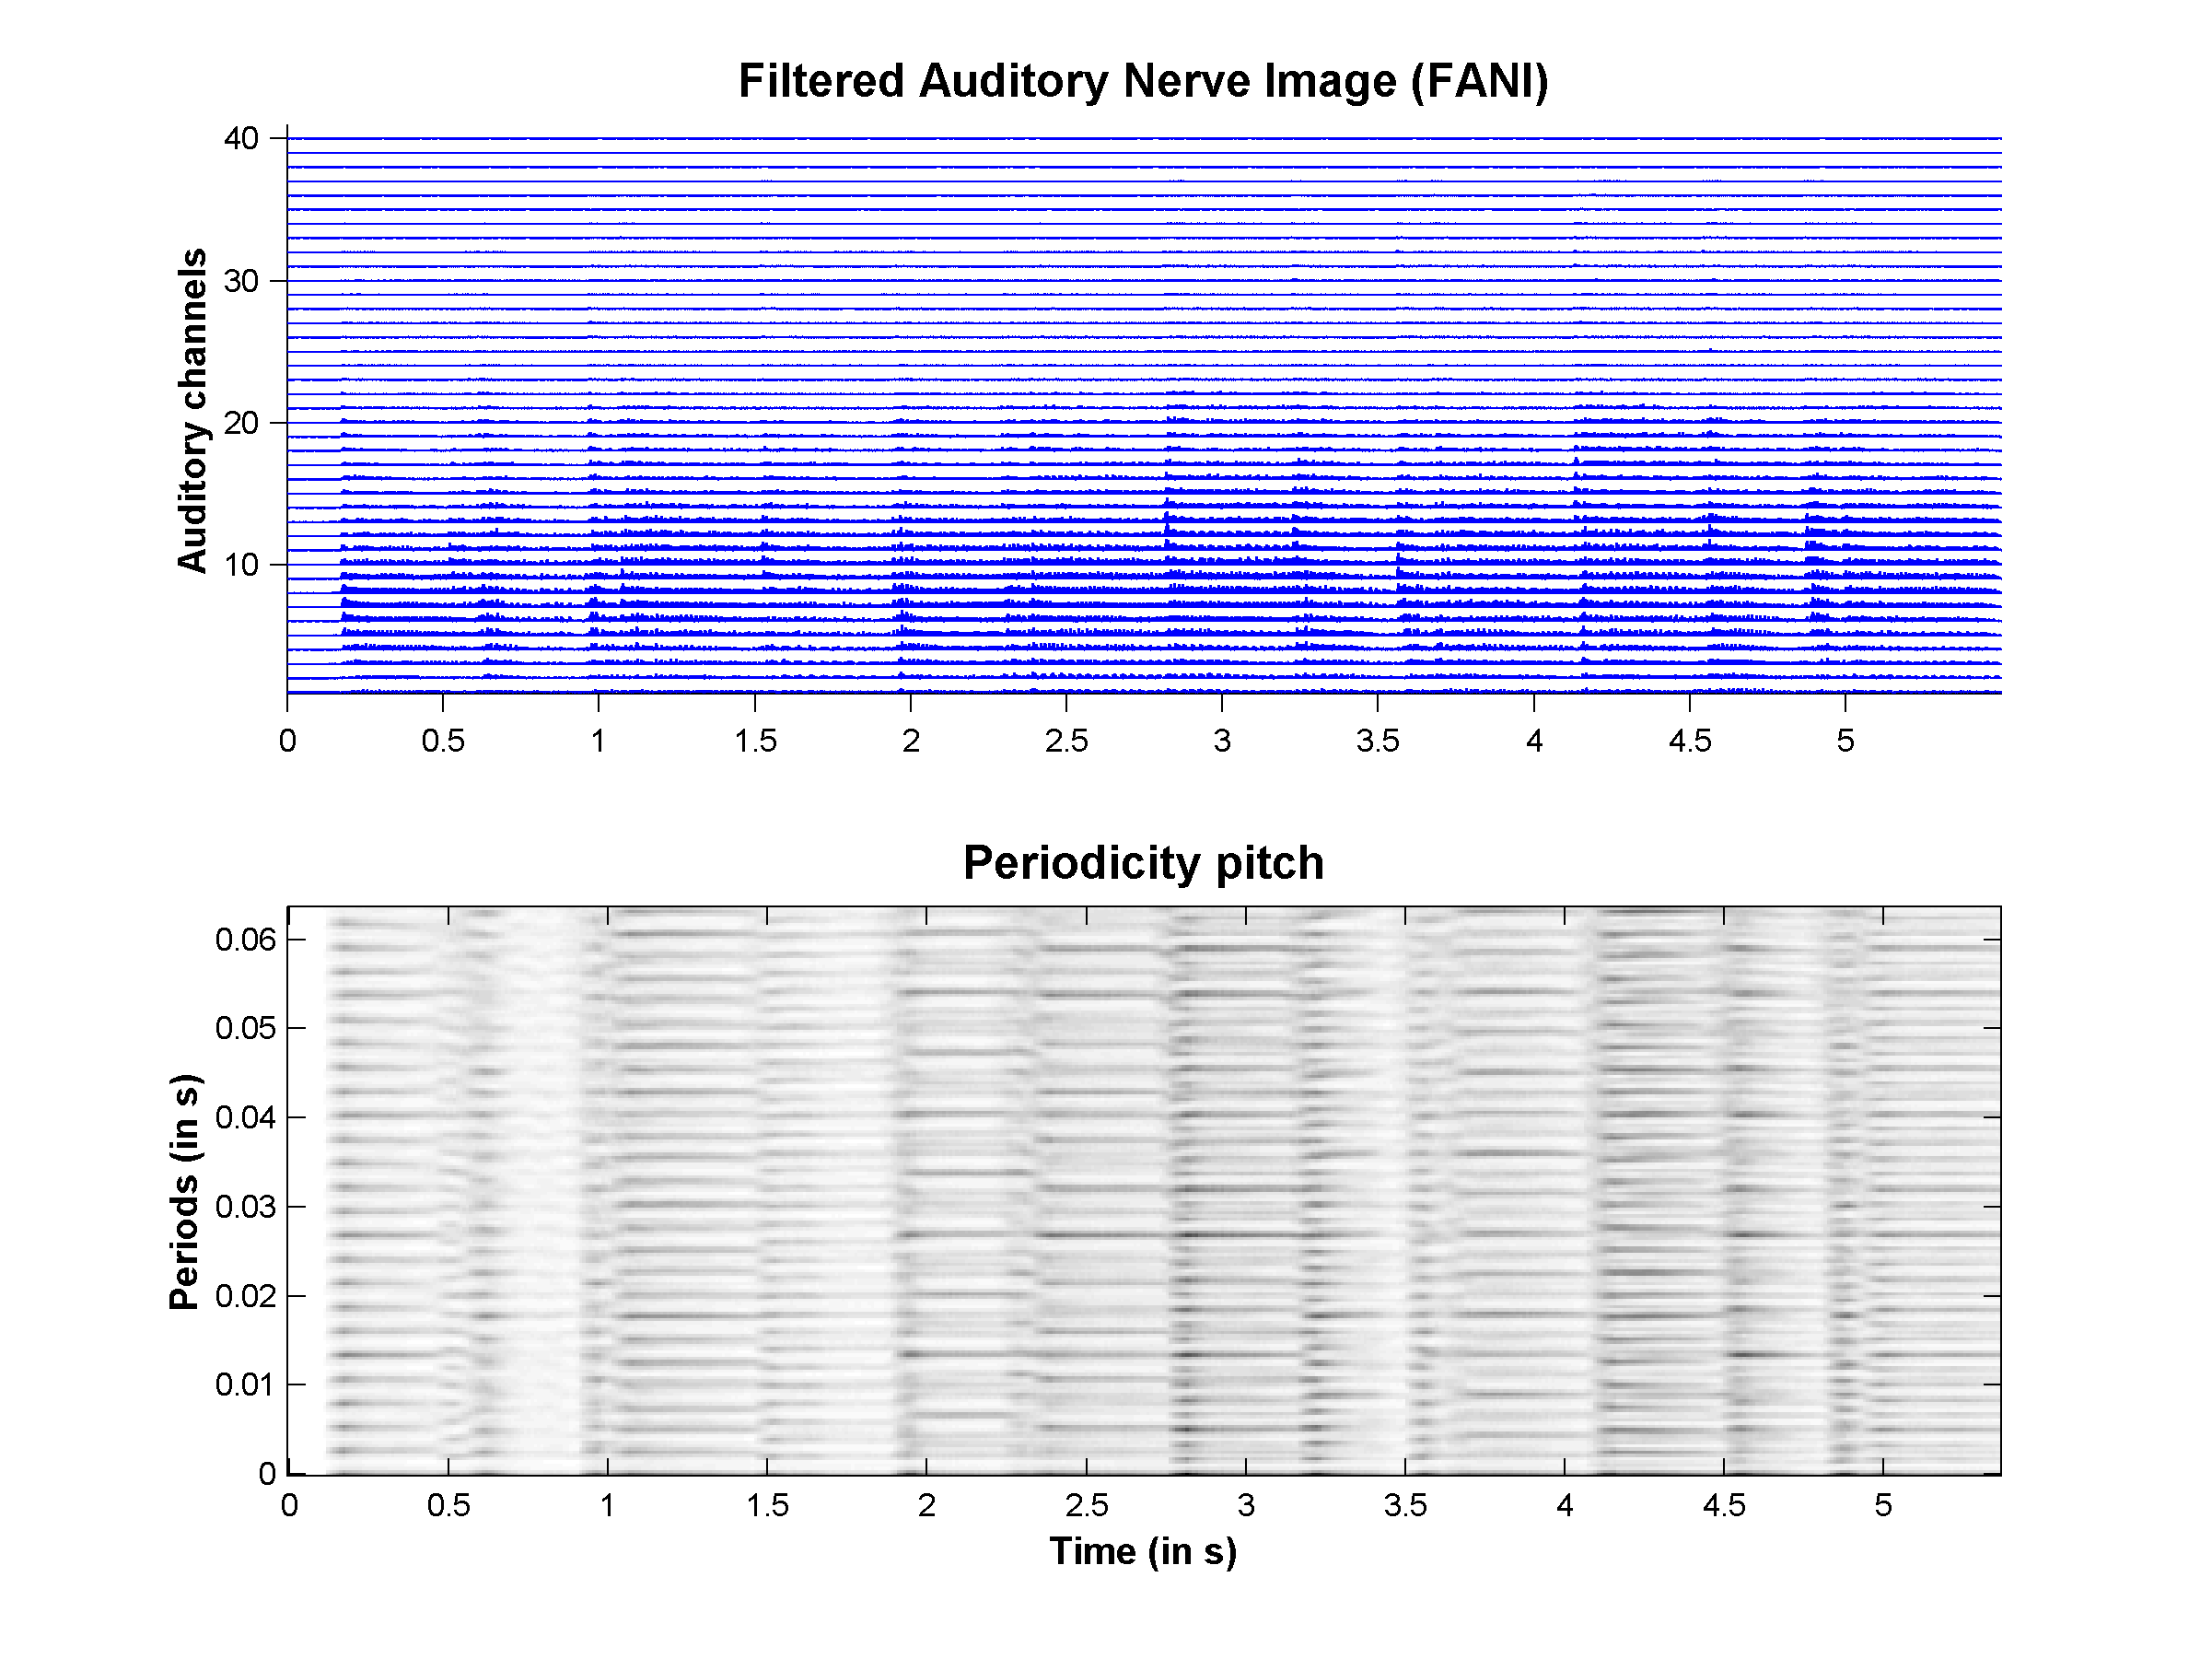
\includegraphics[width=\IPEMDefaultFigureWidth]{Graphics/SchumannPeriodicityPitch}
    \caption{Periodicity Pitch for the excerpt of Schumann's Kuriose Geschichte}
    \label{Fig:SchumannPeriodicityPitch}
\end{figure}

\begin{figure}[h]
    \centering
    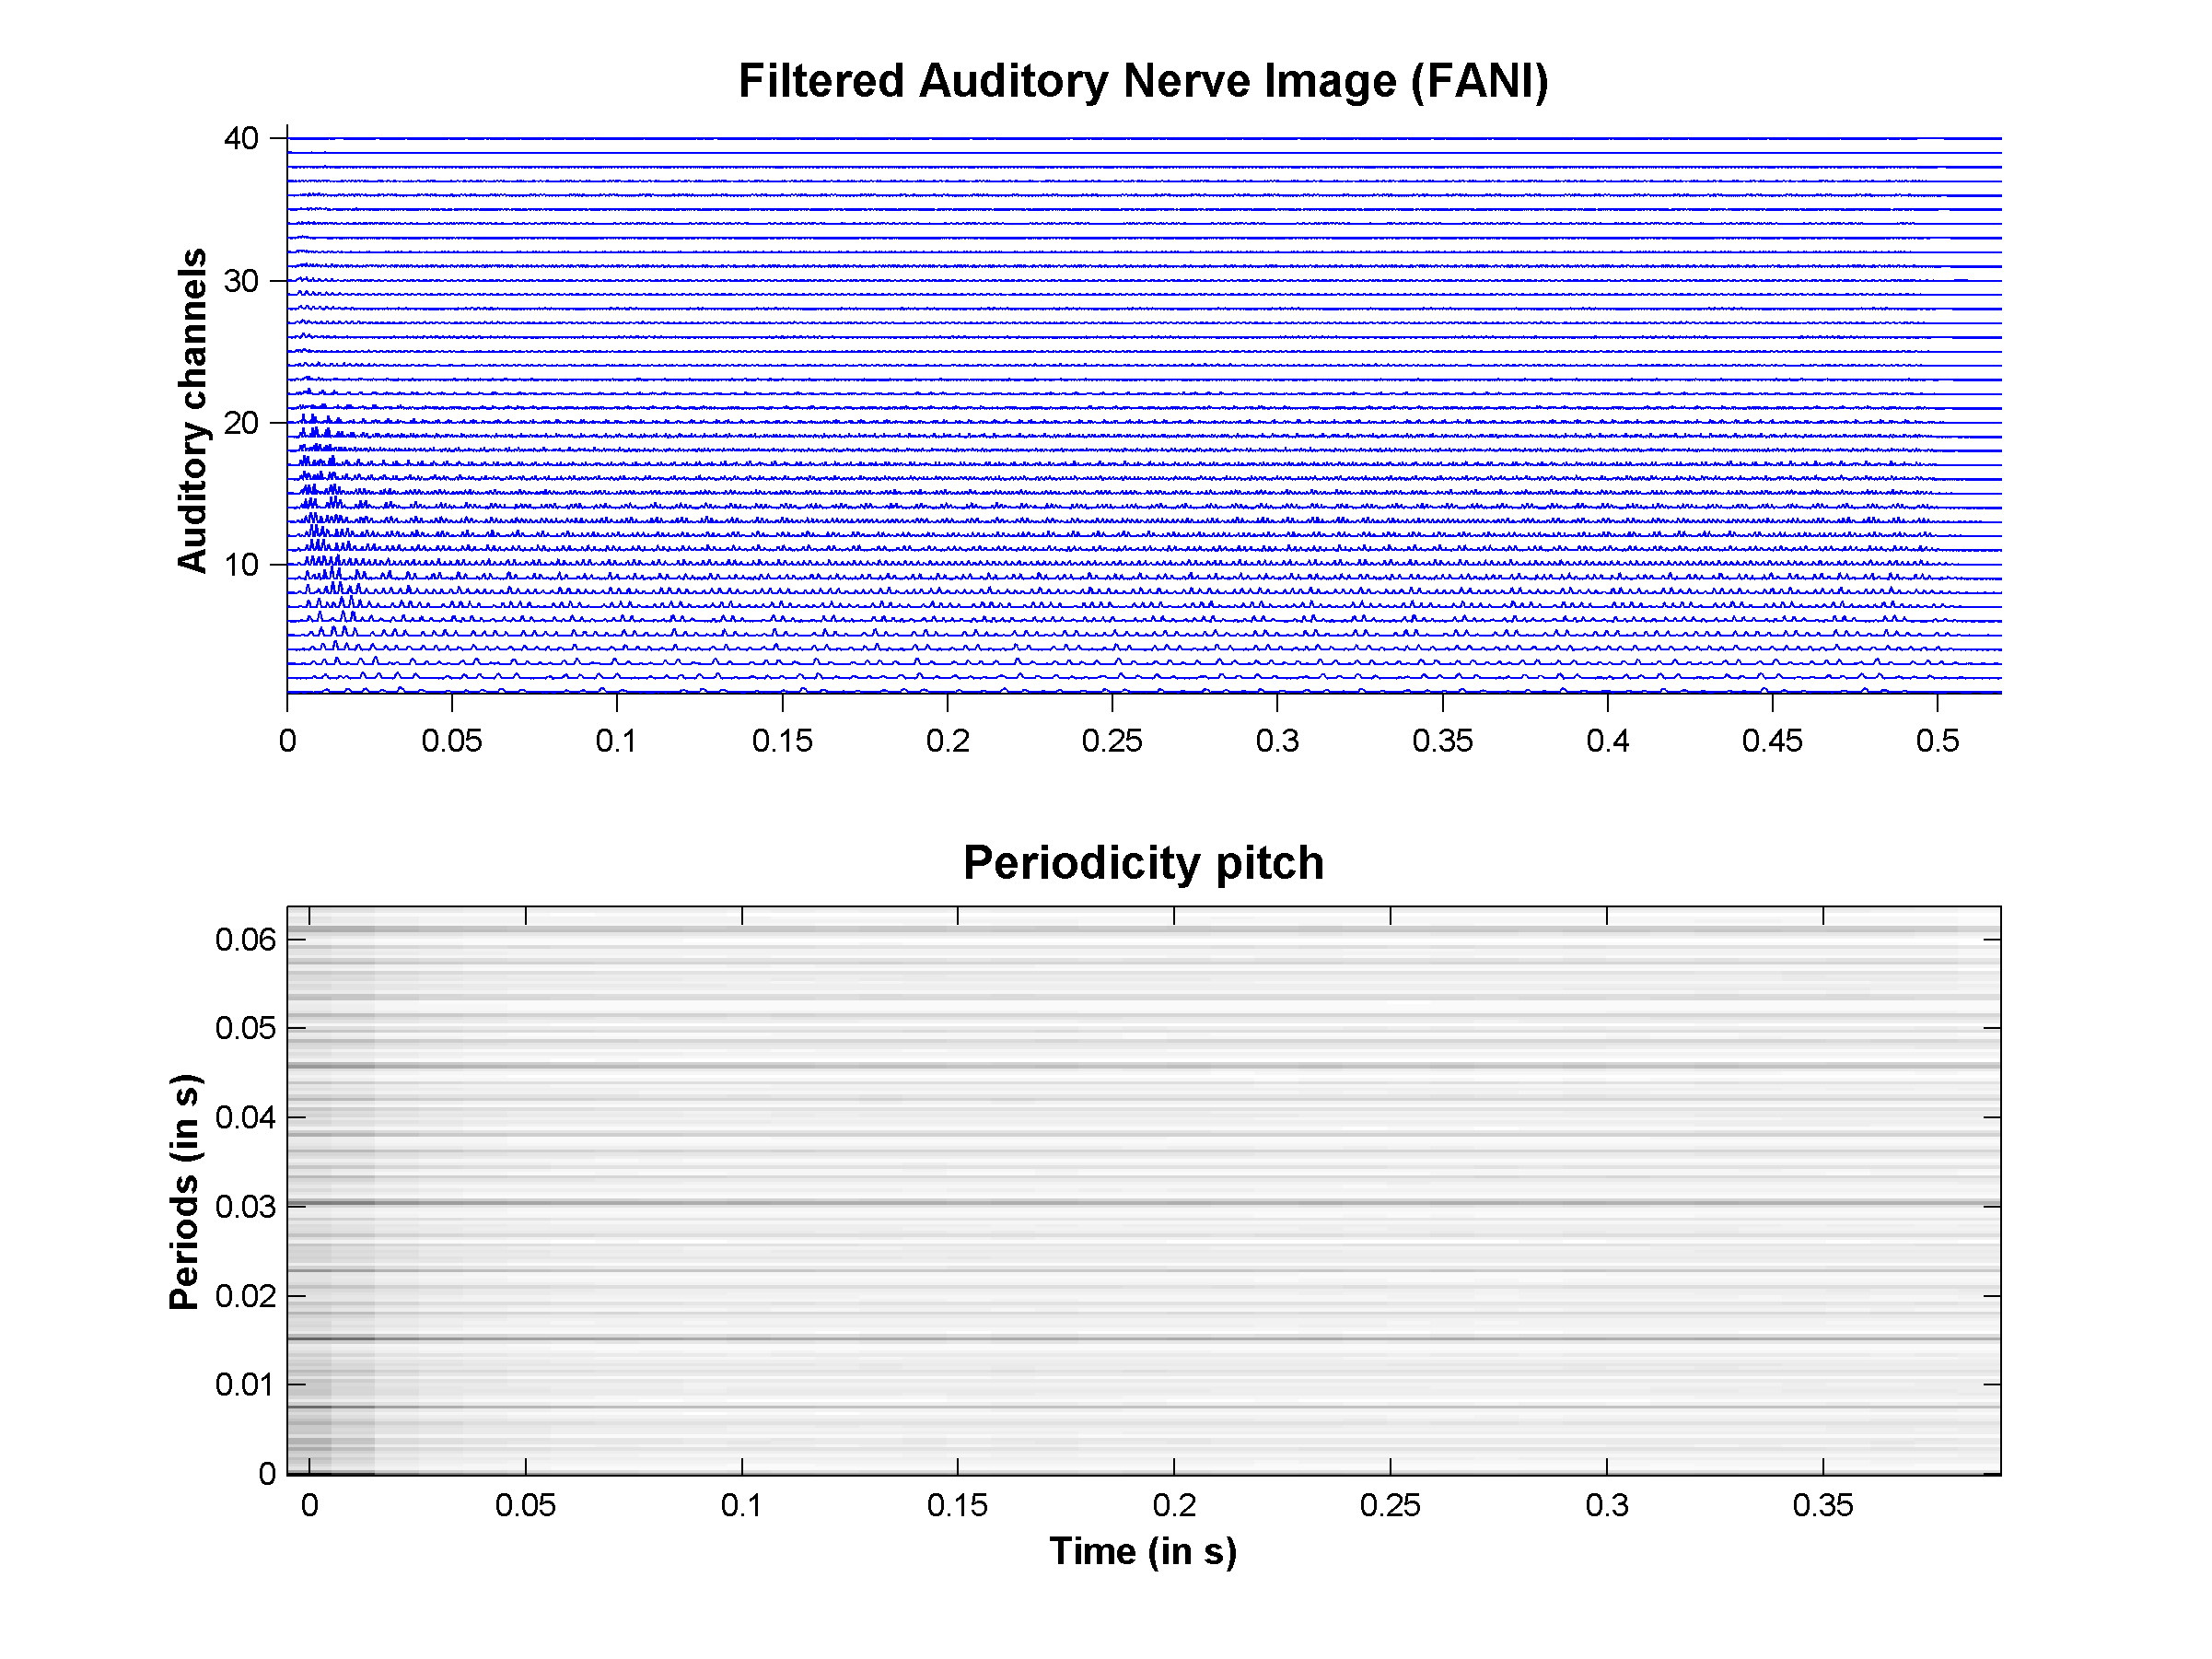
\includegraphics[width=\IPEMDefaultFigureWidth]{Graphics/ShepardCChordPeriodicityPitch}
    \caption{Periodicity Pitch for the C major chord using Shepard tones}
    \label{Fig:ShepardCChordPeriodicityPitch}
\end{figure}

% --------------------------------------------------------------------------------

% --------------------------------------------------------------------------------
% --------------------------------------------------------------------------------
\newpage
\section{Rhythm Module}
% --------------------------------------------------------------------------------

% Make general target
\hypertarget{Concepts:RhythmModule}{}

% Make target for following functions:
\hypertarget{Concepts:IPEMMECAnalysis}{}
\hypertarget{Concepts:IPEMMECExtractPatterns}{}
\hypertarget{Concepts:IPEMMECReSynthUI}{}
\hypertarget{Concepts:IPEMMECSynthesis}{}
\hypertarget{Concepts:IPEMMECSaveResults}{}

% Make target for normal references
\label{Concepts:RhythmModule}

\subsection{Introductory description}
% --------------------------------------------------------------------------------

The Rhythm Module (RhM) uses the Minimal Energy Change (MEC)
algorithm to calculate the fundamental period of a signal. The
input is a sound file and the output is an estimation of the
fundamental period at each time step. The technique used is a
generalization of the Average Magnitude Difference Function, known
as AMDF \cite{inproceedings:LemanVerbeke:Ieper:2000}. The basic
idea is that:
\begin{itemize}
\item
the energy calculated over the period of a repeating pattern is
more or less the same at each moment in time
\item
minimal changes of this energy point to the period of the
repetitive pattern.
\end{itemize}
In applying MEC to rhythm detection we perform the analysis on
the energy patterns in the auditory nerve images. This module
then has its place in the image transformation chart as shown in
figure \ref{Fig:ModulesRhM}.
\begin{figure}[h]
    \centering
    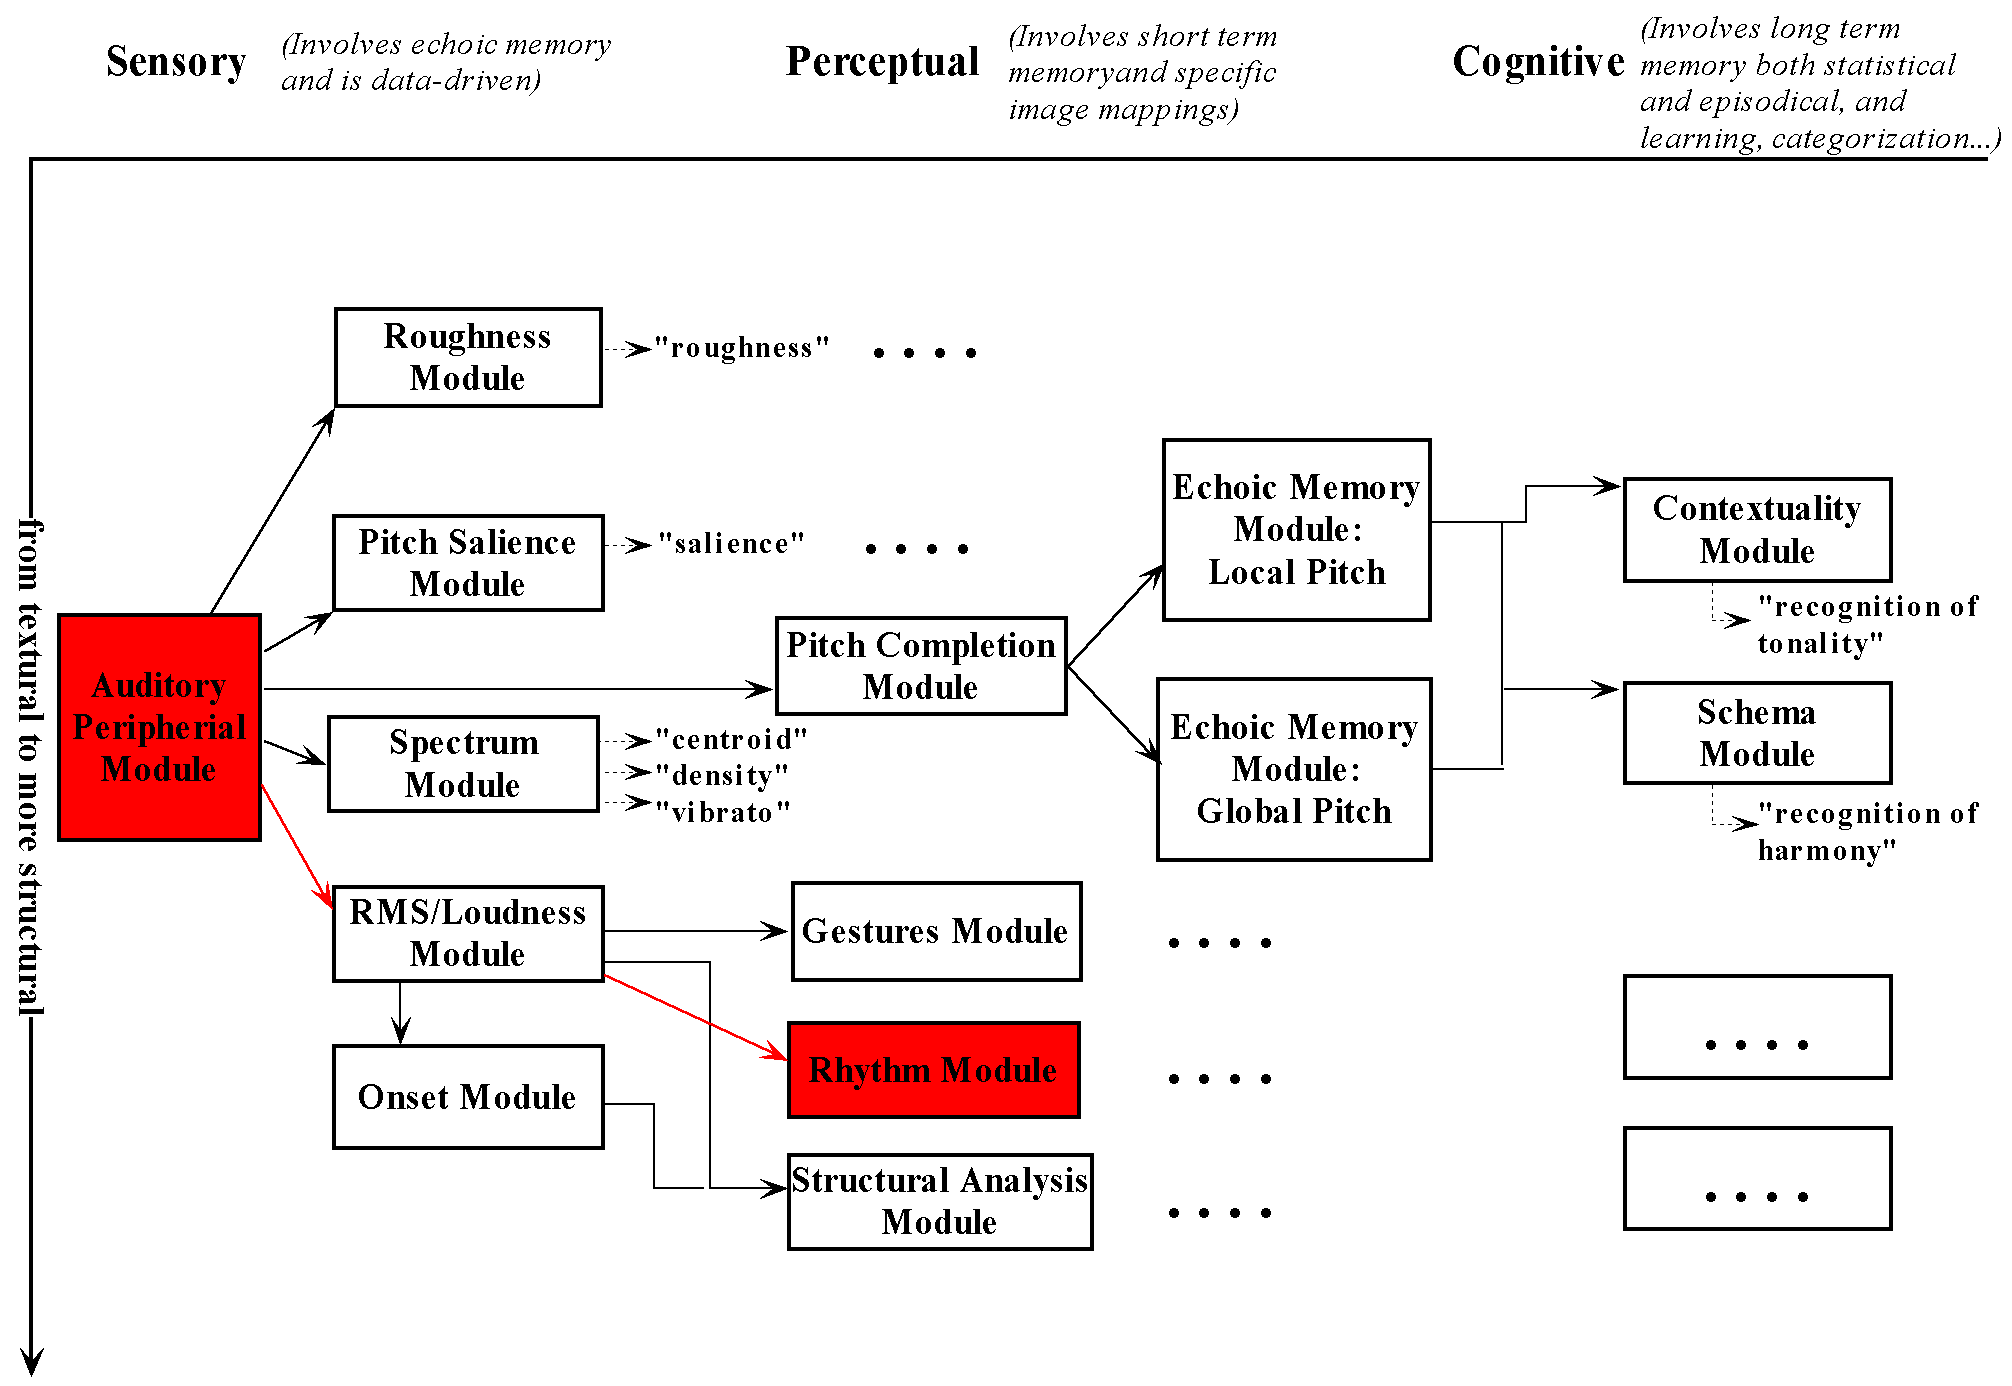
\includegraphics[width=\textwidth]{Graphics/ModulesRhM}
    \caption{Chart of image transformation modules, with RhM highlighted}
    \label{Fig:ModulesRhM}
\end{figure}


\subsection{Functional-logical description}
% --------------------------------------------------------------------------------

The Minimal Energy Change algorithm applied to the recognition of
repetition in rhythm involves:
\begin{eqnarray}
    APM: s(t) \rightarrow e(t,c)\\
    RMS: e(t,c) \rightarrow r(t,c)
\end{eqnarray}
where APM provides the auditory nerve images and where RMS
considers the energy in these images. The application of MEC
involves:
\begin{equation}
    MEC1:  r(t,c) \rightarrow m(\tau,t,c)
\end{equation}
where MEC1 performs a periodicity analysis of these energies and
outputs the estimated periodicity patterns $m(\tau,t,c)$, where
$t$ is time as usual, $\tau$ is the period, and $c$ is the
auditory channel. To obtain the summary MEC-analysis, one has to
sum over all auditory channels, which gives:
\begin{equation}
    MEC2: m(\tau,t) = \sum_{c=1}^{C} m(\tau,t,c)~=~\tilde{m}(t)
\end{equation}
Hence, the MEC-function can be summarized as:
\begin{equation}
    MEC:  \tilde{r}(t) \rightarrow \tilde{m}(t)
\end{equation}
In this notation, one should take into account that the tilde
character, indicating a vector representation, applies to
different dimensions. The components of $\tilde{r}(t)$ are the
channels, while the components of $\tilde{m}(t)$ are the different
periods considered in the analysis. A derived value is the
so-called "best period" $p(t)$, which we obtain by taking the
minimum in each $\tilde{m}(t)$ for fixed $t$, hence:
\begin{equation}
    MEC:  \tilde{r}(t) \rightarrow \tilde{m}(t) \rightarrow p(t)
\end{equation}


\subsection{Signal processing description}
% --------------------------------------------------------------------------------

The MEC-algorithm takes a signal $s(t)$ and its shifted version
$s(t-\tau)$. It then calculates the difference between both
signals, takes the absolute value, and integrates the result:
\begin{equation}\label{MECM1}
    a(\tau,t)~=~
    \int_{0}^{t}~\left|~
    s(t'-\tau)-s(t') ~\right|~
    ~dt'
\end{equation}
where $a(\tau,t)$ at fixed $t$ contains an analysis for all
$\tau$. $\tau$ is typically chosen in the region of interest. For
rhythm detection, this may be from 400 ms to 1 s. The obtained
analysis $a(\tau,t)$ at fixed $t$ is then searched for a minimum:
\begin{equation}\label{MECM2}
    p(t) = ~min_{\tau>0}~a(\tau,t)
\end{equation}
which gives a value $p$ for the best period at each time step $t$.

In practice, we can build in more stability by leaky-integrating
the $a(\tau,t)$ over $t$:
\begin{equation}\label{MECM1B}
    a(\tau,t)~=~
    \int_{0}^{t}~\left|~
    s(t'-\tau)-s(t') ~\right|~
    e^{\beta(t-t')}~dt'
\end{equation}
and apply Expression \ref{MECM2}.

When applied to the signal in different auditory channels, the
calculation will be applied to each channel, thus giving
$a(\tau,t,c)$. To get the best period, one may calculate $p(t)$
using $\sum_{c=1}^{C}a(\tau,t,c)$.


\subsection{Implementation}
% --------------------------------------------------------------------------------

\begin{tabularx}{\linewidth}{llX}
\hyperlink{FuncRef:IPEMMECAnalysis}{IPEMMECAnalysis} & - & Performs a periodicity analysis of a (multi-channel) signal using the MEC model\\
\hyperlink{FuncRef:IPEMMECExtractPatterns}{IPEMMECExtractPatterns} & - & Extracts the best pattern from the original signal using the results of an IPEMMECAnalysis run\\
\hyperlink{FuncRef:IPEMMECReSynthUI}{IPEMMECReSynthUI} & - & User interface callback function for interactively handling the resynthesis of MEC analysis results\\
\hyperlink{FuncRef:IPEMMECSaveResults}{IPEMMECSaveResults} & - & Utility function that saves the results of IPEMMECExtractPatterns, so that resynthesis can still be done at a later date, after reloading this data\\
\hyperlink{FuncRef:IPEMMECSynthesis}{IPEMMECSynthesis} & - & Generates an AM modulated noise signal constructed from a repetition of the pattern found at the specified time moment\\
\end{tabularx}


\subsection{Examples}
% --------------------------------------------------------------------------------

The first steps involve the preparation of the signal in which we
want to look for periodicity. This is done by:\\

\begin{IPEMCodeEnvironment}
[ANI,ANIFreq,ANIFilterFreqs] = IPEMCalcANIFromFile('SchumannKurioseGeschichte.wav');
\newline [RMS,RMSFreq] = IPEMCalcRMS(ANI,ANIFreq,0.050,0.020);
\newline [Periods,Best,AnalysisFreq,Values] = IPEMMECAnalysis(RMS,RMSFreq,0.5,3,[],1.5);
\end{IPEMCodeEnvironment}\\

The MEC algorithm has stored the periods that were analyzed in
\IPEMCodeExtract{Periods}, the indices (into
\IPEMCodeExtract{Periods}) for the best periods found in each
channel in \IPEMCodeExtract{Best}, and all values $m(\tau,t,c)$ in
\IPEMCodeExtract{Values}. The data format of
\IPEMCodeExtract{Values} is described in
\hyperlink{FuncRef:IPEMMECAnalysis}{IPEMMECAnalysis}. Just to give
you an example of how to work with MATLAB, we sum over all
channels $c$ in the following way:\\

\begin{IPEMCodeEnvironment}
SummaryPeriodicity = zeros(size(Values\{1\}));
\newline for channel = 1:40;
\newline SummaryPeriodicity = SummaryPeriodicity + Values\{channel\};
\newline end
\end{IPEMCodeEnvironment}\\

The values in \IPEMCodeExtract{SummaryPeriodicity} contain the
periodicity analysis over all channels which can be visualized
using the MATLAB code:\\

\begin{IPEMCodeEnvironment}
figure;
\newline imagesc((0:size(SummaryPeriodicity,2)-1)/AnalysisFreq,Periods,SummaryPeriodicity);
\newline xlabel('Time (in s)'); ylabel('Period (in s)');
\newline axis xy; colormap(1-gray);
\end{IPEMCodeEnvironment}\\

We plot the best periods of the summary periodicity on top of the
image.\\

\begin{IPEMCodeEnvironment}
[M,I]=min(SummaryPeriodicity); hold on;
\newline plot((0:length(I)-1)/AnalysisFreq,Periods(I));
\end{IPEMCodeEnvironment}\\

The resulting graph should be similar to the one in figure
\ref{Fig:RhMDifferenceValuesSchumannn}.

\begin{figure}[h]
    \centering
    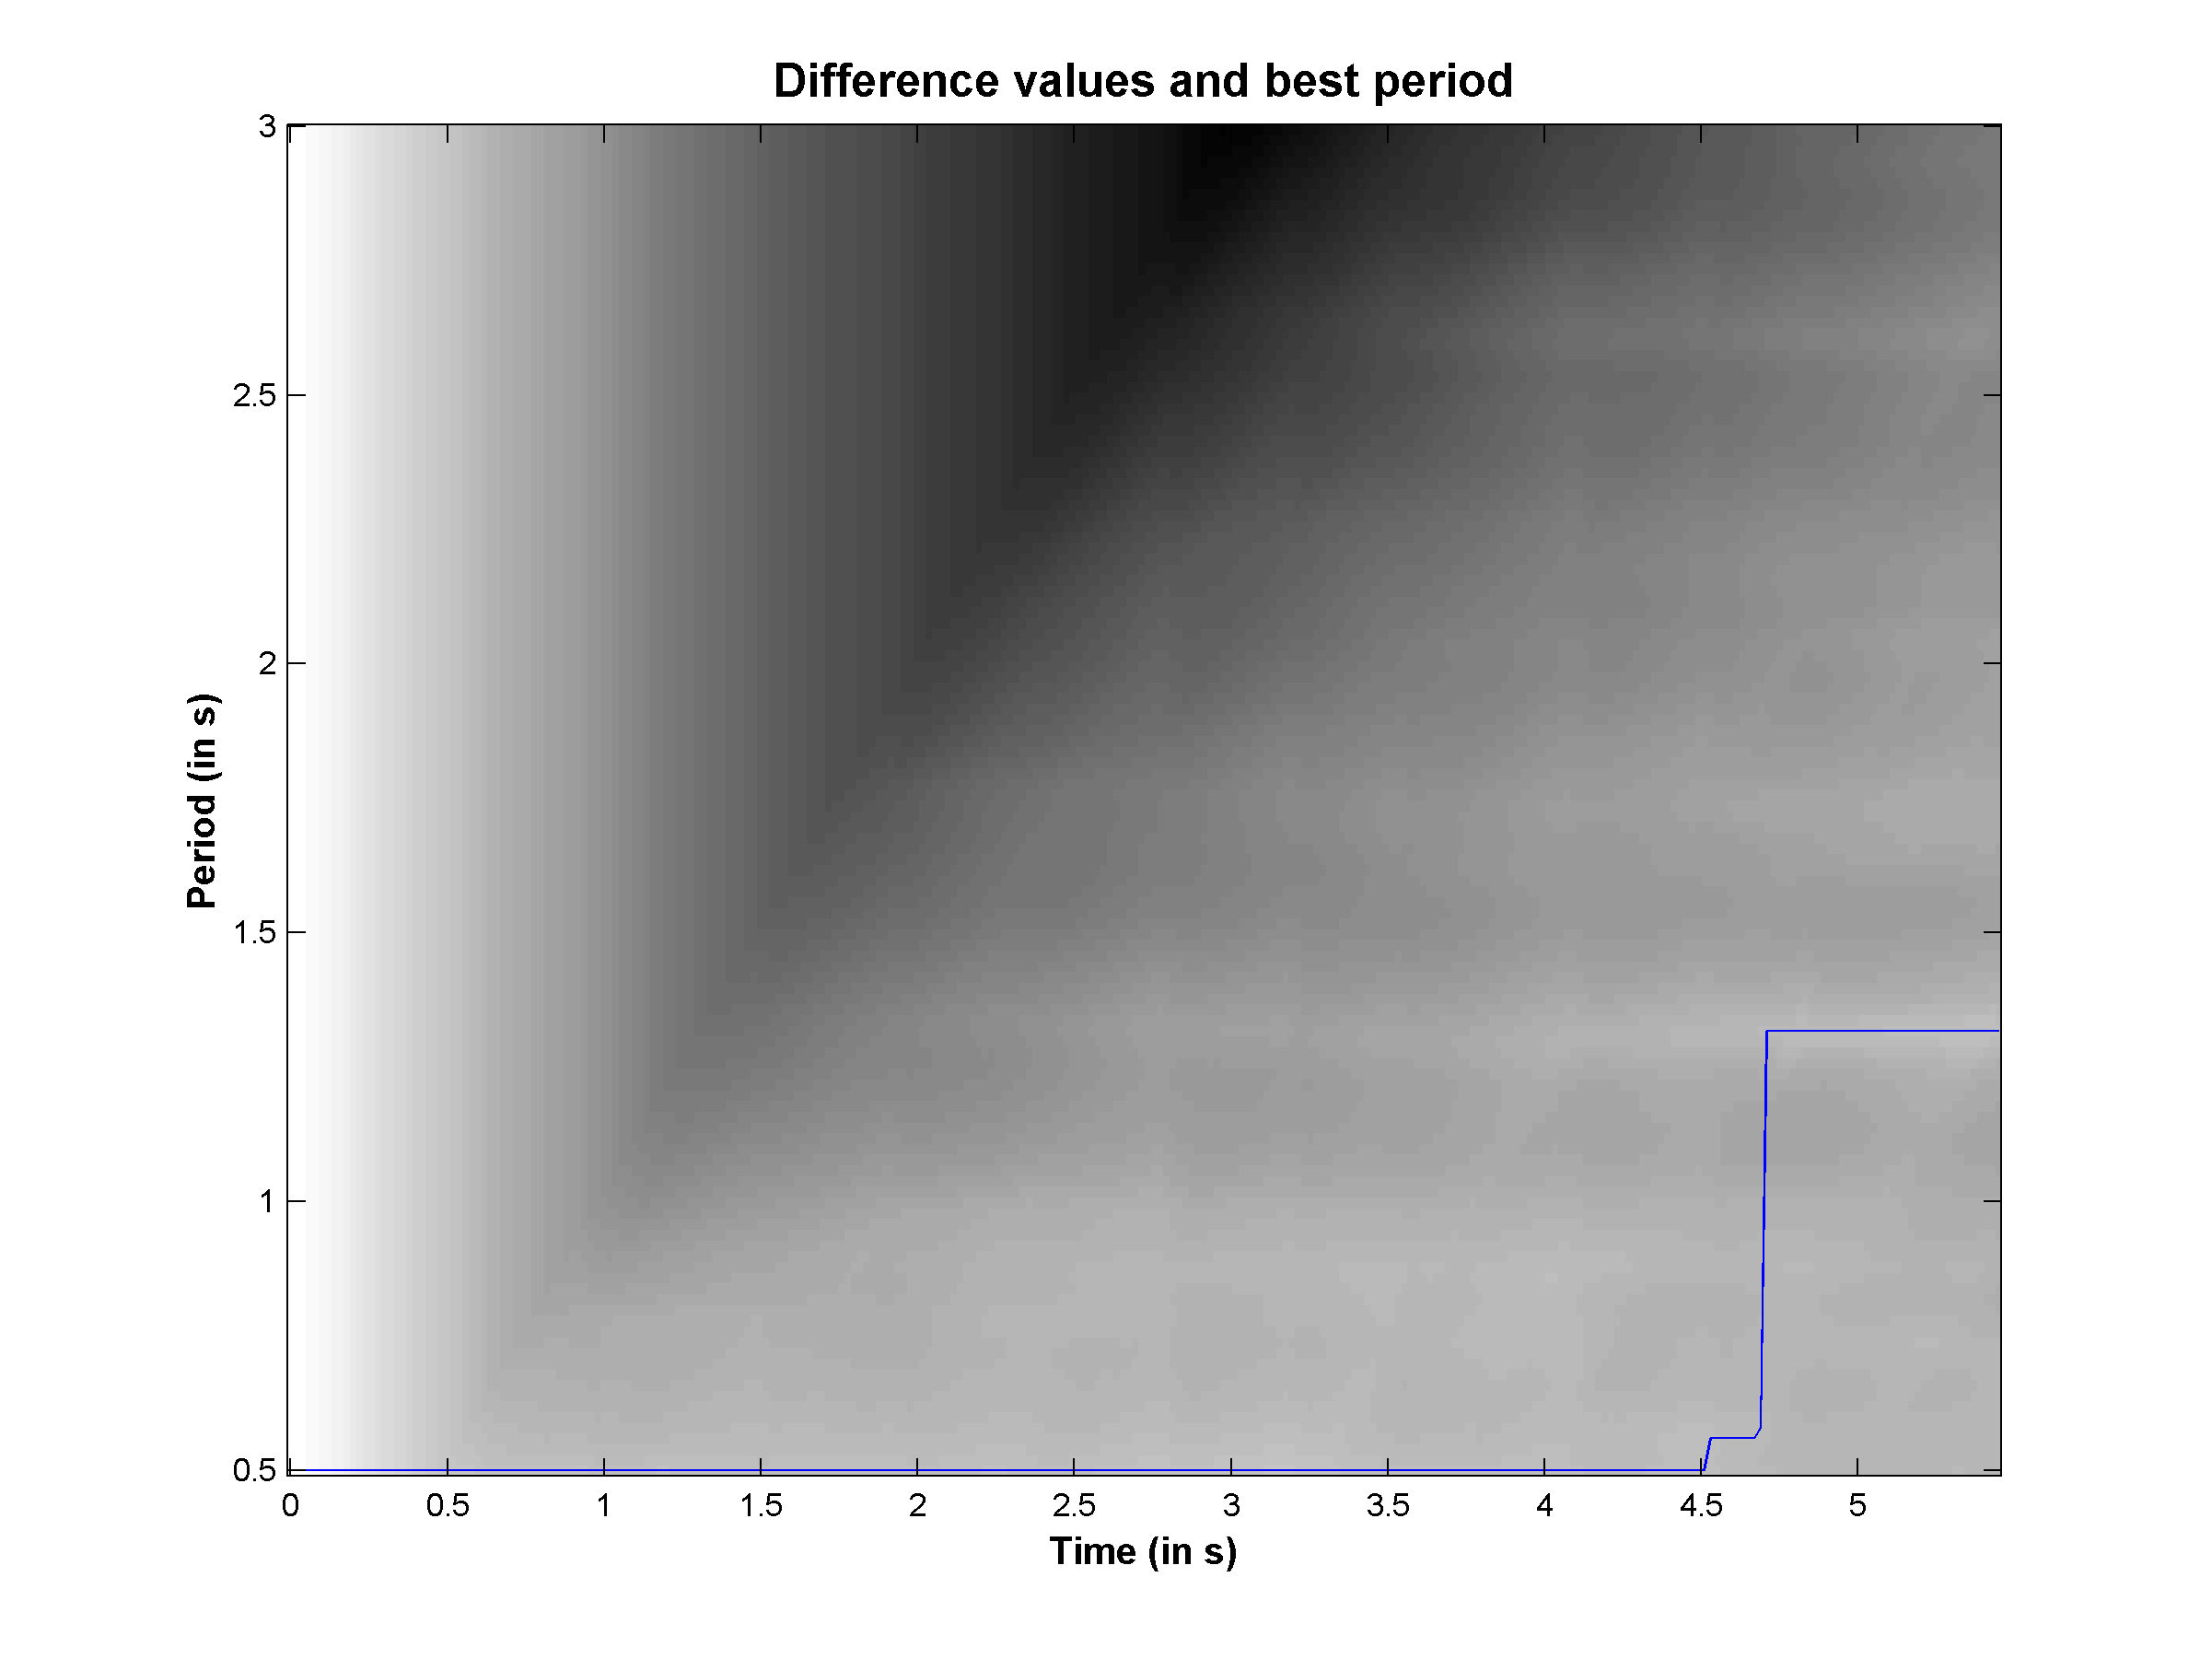
\includegraphics[width=\IPEMDefaultFigureWidth]{Graphics/RhMDifferenceValuesSchumannn}
    \caption{MEC analysis result of a short excerpt of Schumann's Kuriose Geschichte. Shown are the summed difference values (over all channels) and a plot of the best period on top of this.}
    \label{Fig:RhMDifferenceValuesSchumannn}
\end{figure}

% --------------------------------------------------------------------------------

% --------------------------------------------------------------------------------
% --------------------------------------------------------------------------------
\newpage
\section{Echoic Memory Module}
% --------------------------------------------------------------------------------

% Make general target
\hypertarget{Concepts:EchoicMemoryModule}{}

% Make target for following functions:
\hypertarget{Concepts:IPEMLeakyIntegration}{}

\subsection{Introductory description}
% --------------------------------------------------------------------------------

An echo can be defined as a leaky integration with a given half
decay time. At each moment in time, a leaky integrator adds the
incoming signal value to an attenuated version of the previously
calculated value to form the newly calculated value. The half
decay time specifies the time it takes for an impulse signal to
reach half its original value.

The Echoic Memory Module (EMM) takes an image as input and gives
the leaky integrated image as output. The images are integrated so
that at each time step, the new image is calculated by taking a
certain amount of the old image which is then added with the new
incoming image.

The Echoic Memory Module can be applied to pitch completion
images, for example. We then start from our familiar APM, followed
by PCM, and apply EMM. The echo which we specify defines the
amount of context which we take into account. With very little (or
almost no) context we speak about \emph{local pitch images}. When
context is taken into account we use a longer half decay time and
call the images \emph{global pitch images}. EMM has been used in
\citeA{article:MusicPerception:Leman:2000} to construct the
pitch images of an echoic memory. In our global chart of image
transformation modules EMM is localized in the middle part
(perception section) of figure \ref{Fig:ModulesEMM}. The
application is described in detail in the chapter on
\hyperlink{Concepts:IPEMGenerateProbes}{{tonality induction
experiments}}.
\begin{figure}[h]
    \centering
    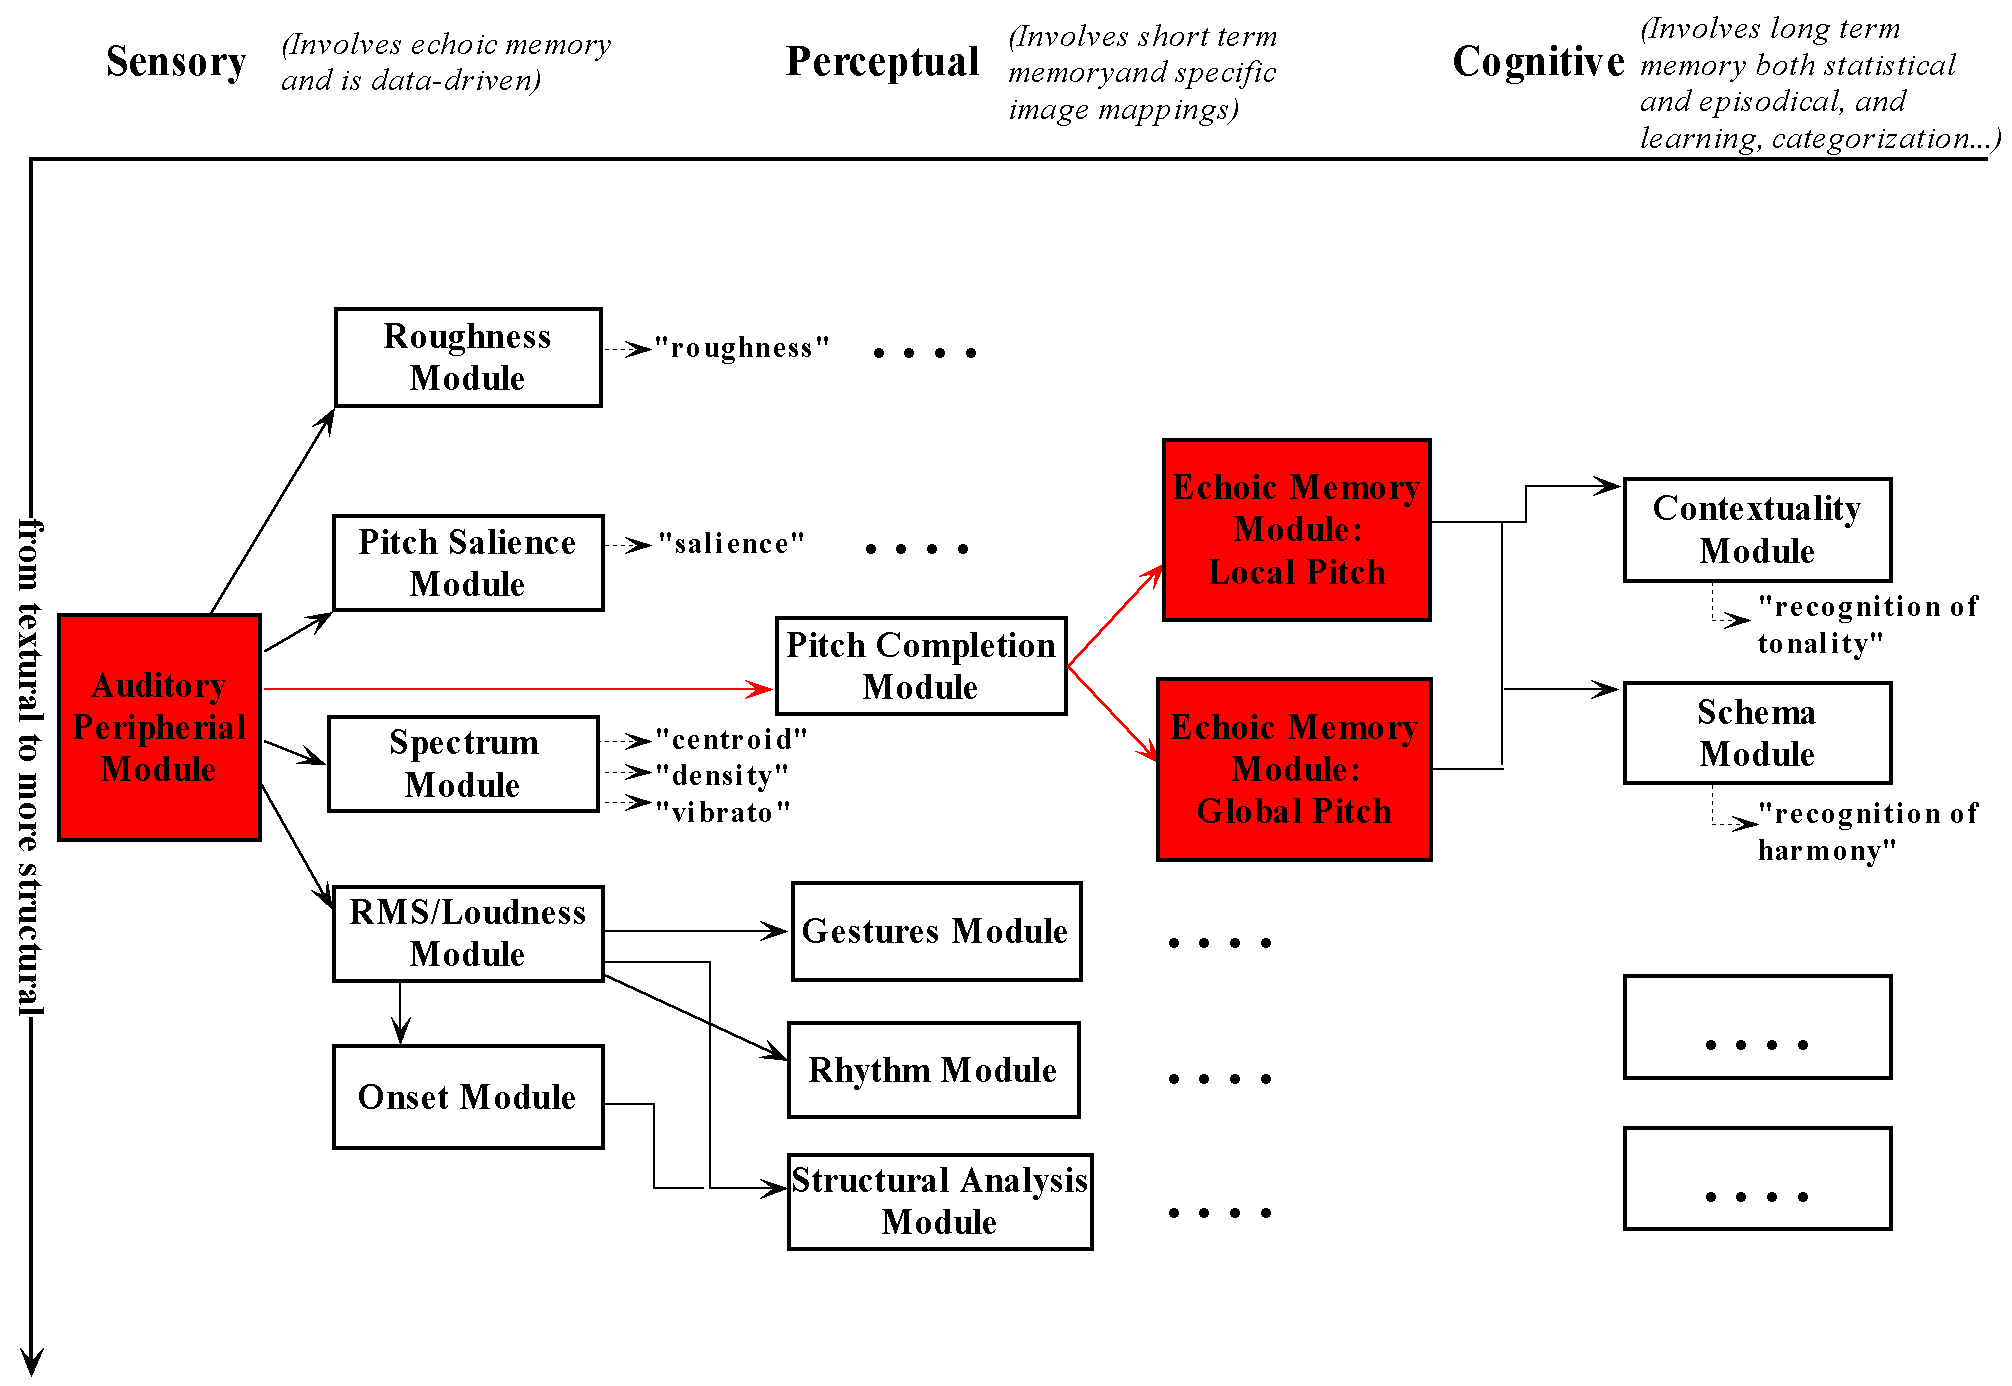
\includegraphics[width=\textwidth]{Graphics/ModulesEMM}
    \caption{Chart of image transformation modules, with EMM highlighted}
    \label{Fig:ModulesEMM}
\end{figure}
Figure \ref {Fig:EMMModule} shows the modules involved in the
image transformation process.
\begin{figure}[h]
    \centering
    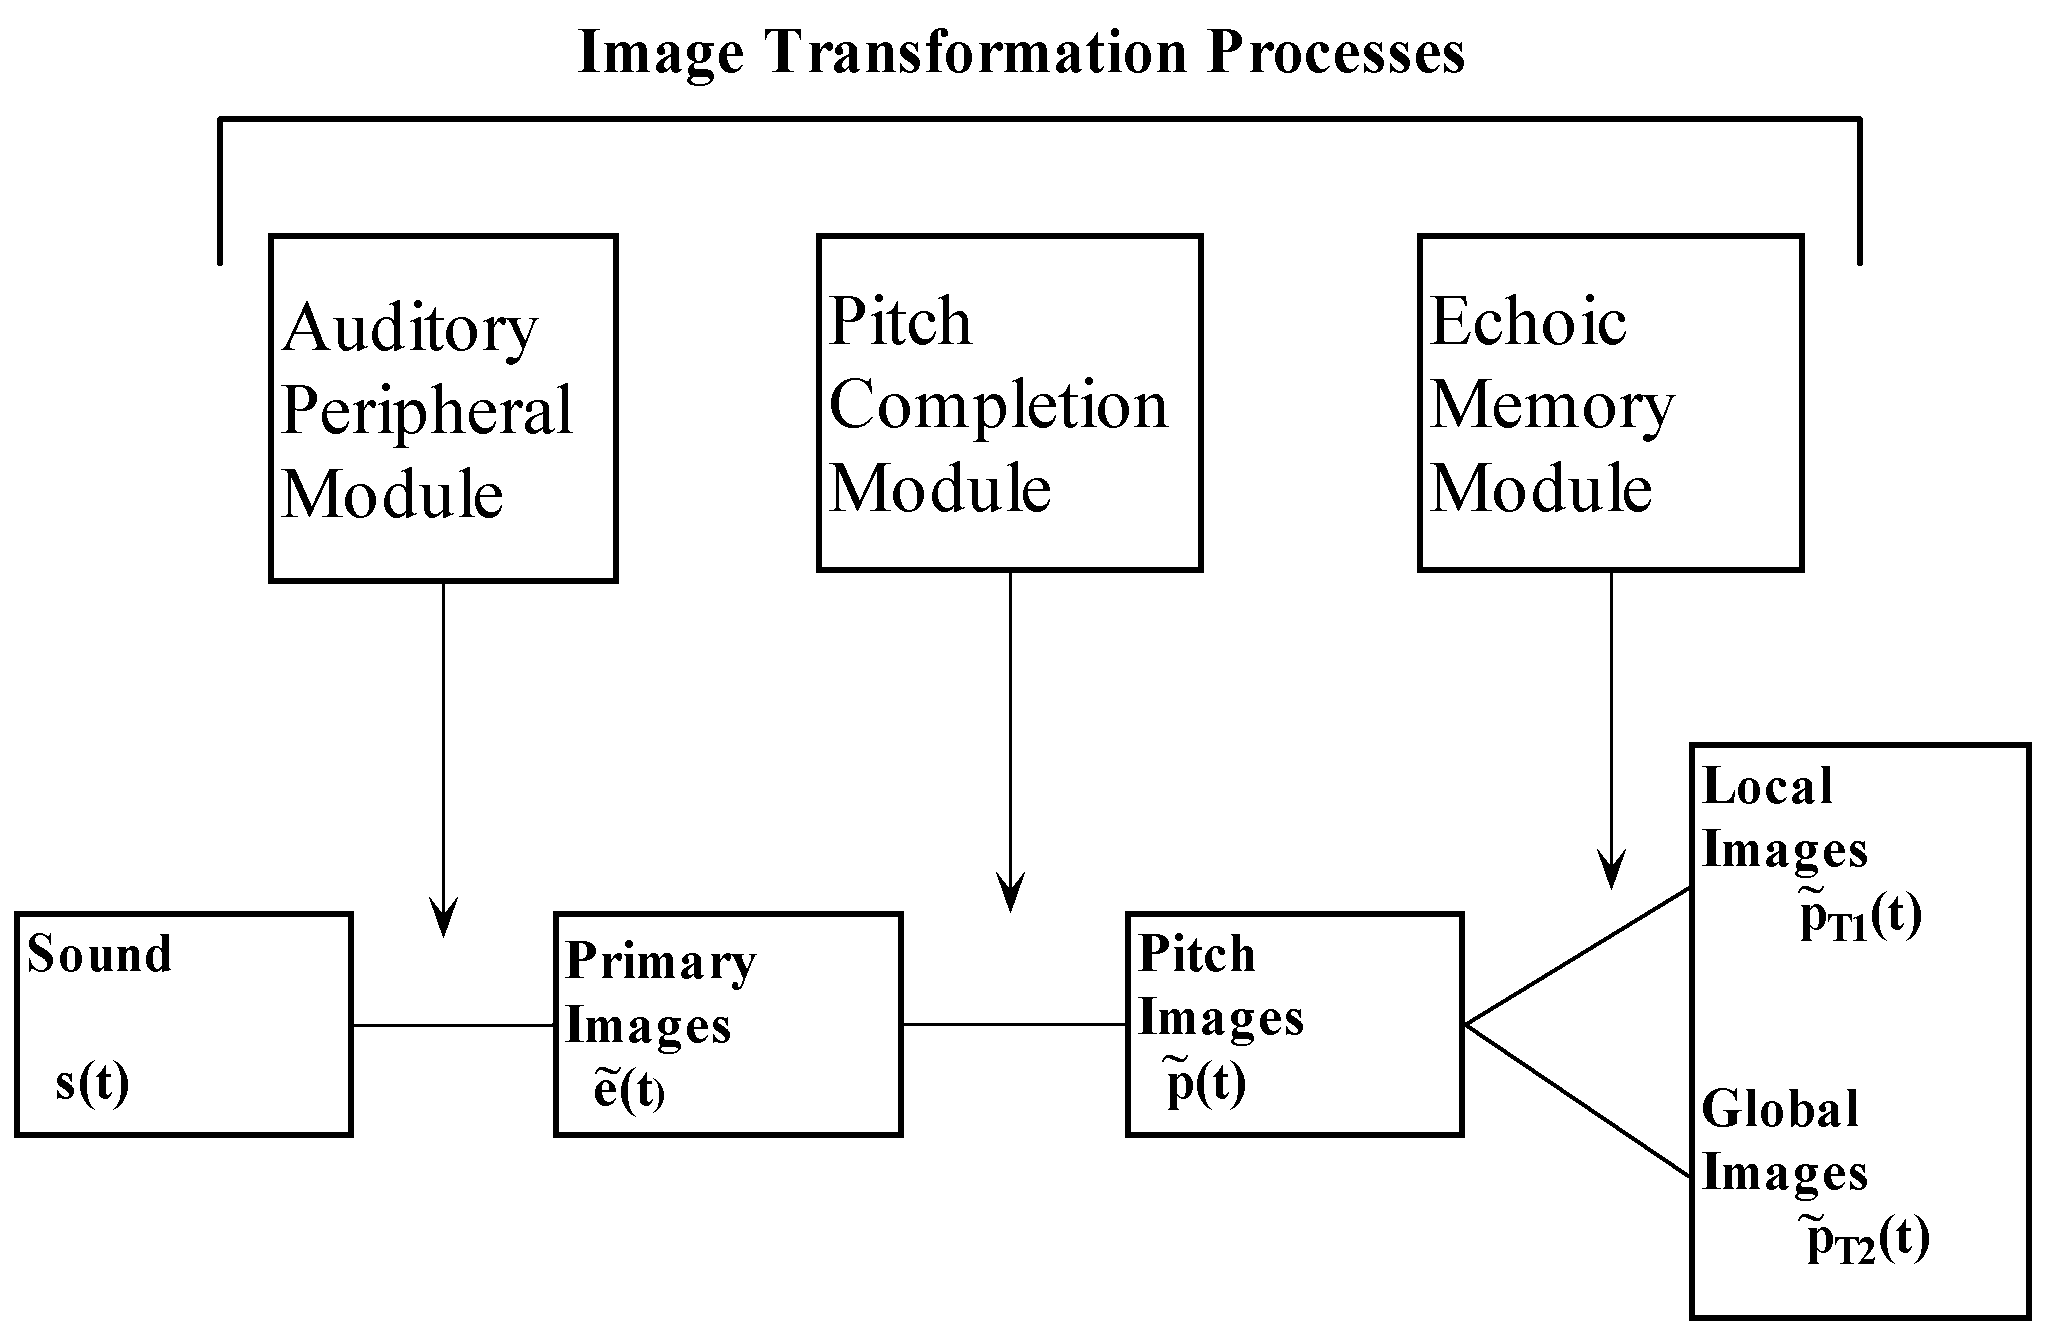
\includegraphics[width=\IPEMDefaultFigureWidth]{Graphics/EMMModule}
    \caption{Image Transformation Process: Echoic Memory Module}
    \label{Fig:EMMModule}
\end{figure}

\subsection{Functional-logical description}
% --------------------------------------------------------------------------------

A symbolic representation of the Echoic Memory Module may be written as:
\begin{equation}
EMM: \tilde{p}(t) \rightarrow \tilde{p}_T(t)
\end{equation}
where $T$ denotes the {\sl echo} in seconds, $\tilde{p}(t)$
denotes a pitch completion image and $ \tilde{p}_T(t)$ an echoed
image.


\subsection{Signal processing description}
% --------------------------------------------------------------------------------

$\tilde{p}_T(0) = \tilde{p}(0)$

$\tilde{p}_T(t) = \tilde{p}(t) ~+~
\tilde{p}_T(t-1)*2^{\frac{-1}{T}}$ \quad , $t \neq 0$


\subsection{Implementation}
% --------------------------------------------------------------------------------

\begin{tabularx}{\linewidth}{llX}
\hyperlink{FuncRef:IPEMLeakyIntegration}{IPEMLeakyIntegration} & - & Calculates leaky integration with specified half decay time\\
\end{tabularx}


\subsection{Examples}
% --------------------------------------------------------------------------------

The Echoic Memory Module can be applied to a pitch completion
image to obtain a local and a global pitch image. A local pitch
image can be defined as $\tilde{p}_{T=0.1}(t)$, with an echo of
0.1 s, while a global pitch image can be defined as
$\tilde{p}_{T=1.5}(t)$, with the echo of 1.5 s. Local images are
built up by echoes which, by definition, are smaller than echoes
for the global images. Use the following MATLAB functions to
create those pitch images:\\

\begin{IPEMCodeEnvironment}
[ANI,ANIFreq,ANIFilterFreqs] = IPEMCalcANIFromFile('SchumannKurioseGeschichte.wav');
\newline [PP,PPFreq,PPPeriods,PPFANI] = IPEMPeriodicityPitch(ANI,ANIFreq);
\newline LocalIntegration = IPEMLeakyIntegration(PP,PPFreq,0.1,0.1,1);
\newline GlobalIntegration = IPEMLeakyIntegration(PP,PPFreq,1.5,1.5,1);
\end{IPEMCodeEnvironment}\\

Figure \ref{Fig:EMMPitchImages} shows the pitch images for the
\IPEMSound{Sounds/SchumannKurioseGeschichte.wav}{excerpt of
Schumann's Kuriose Geschichte}.

\begin{figure}[h]
    \centering
    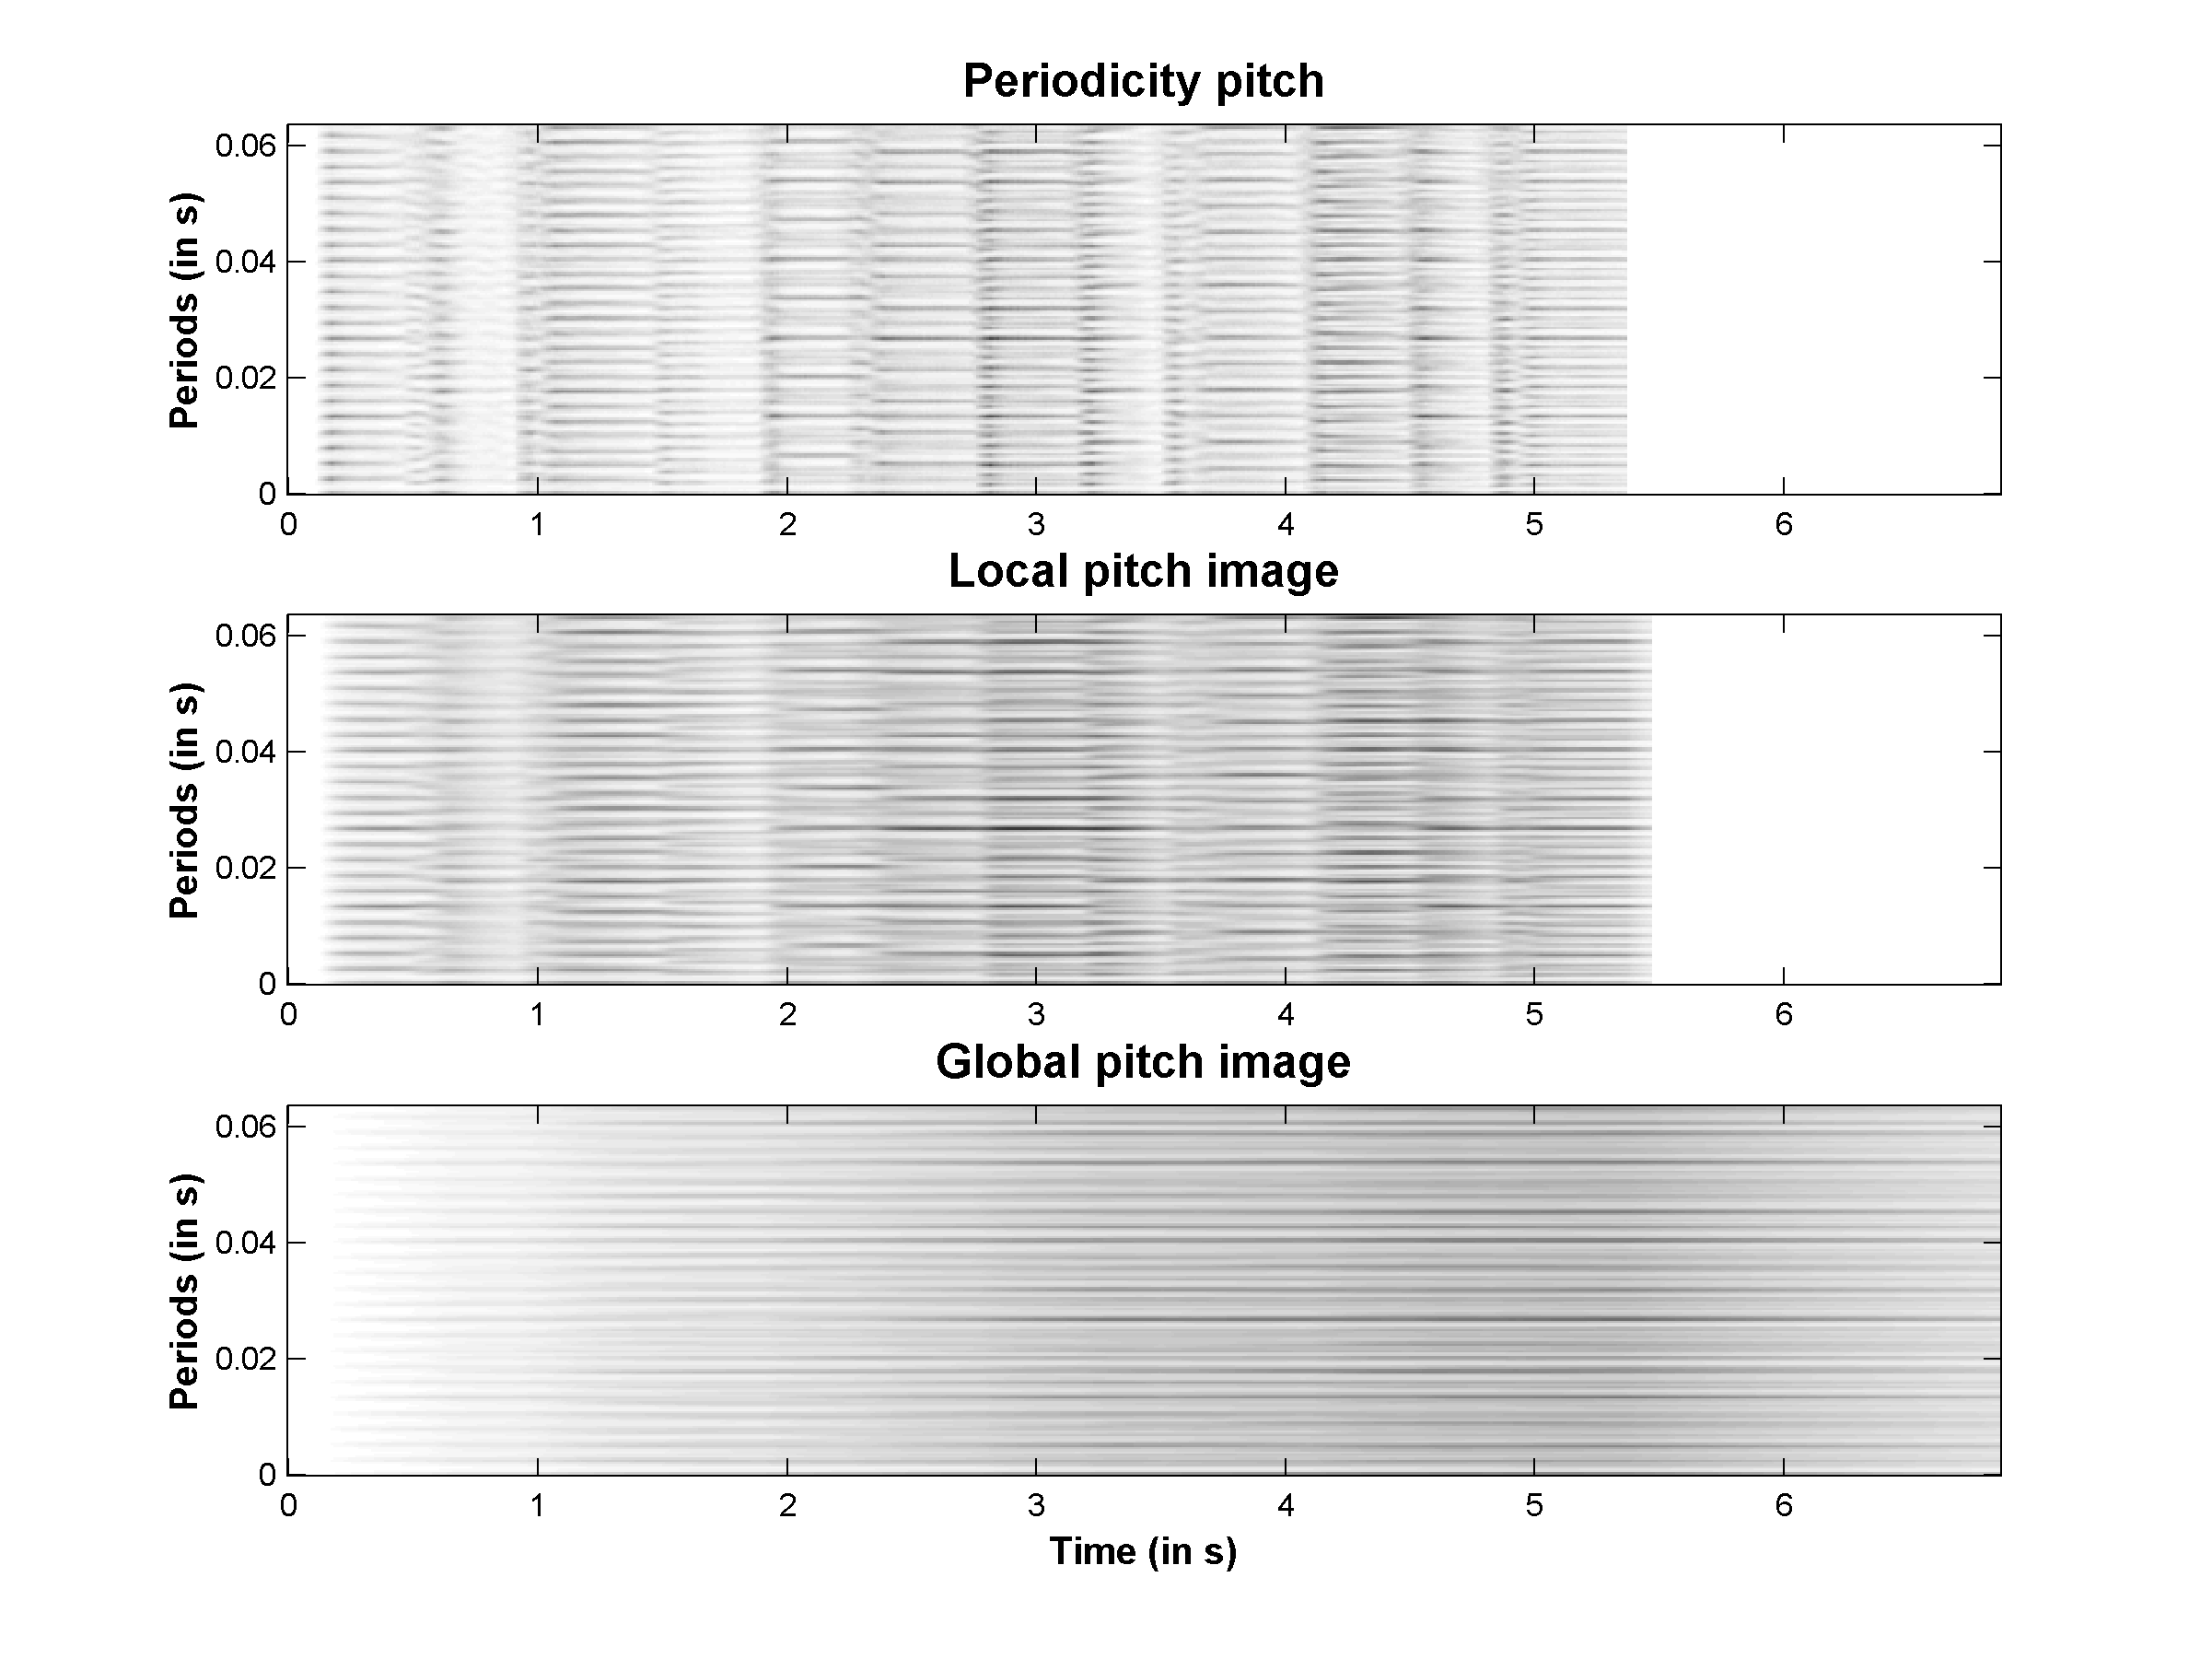
\includegraphics[width=\IPEMDefaultFigureWidth]{Graphics/EMMPitchImages}
    \caption{Top: periodicity pitch for the excerpt of Schumann's Kuriose Geschichte
    Middle: local pitch image of Schumann's Kuriose Geschichte (echo of 0.1 s).
    Bottom: global pitch image (echo of 1.5 s)}
    \label{Fig:EMMPitchImages}
\end{figure}

% --------------------------------------------------------------------------------

% --------------------------------------------------------------------------------
% --------------------------------------------------------------------------------
\newpage
\section{Contextuality Module}
% --------------------------------------------------------------------------------

% Make general target
\hypertarget{Concepts:ContextualityModule}{}

% Make target for following functions:
\hypertarget{Concepts:IPEMContextualityIndex}{}

\subsection{Introductory description}
% --------------------------------------------------------------------------------

Contextuality measures the pitch commonality between two running
pitch images of the same sound, each having a possible different
echo. In \citeA{article:MusicPerception:Leman:2000}, contextuality
is used to measure the pitch commonality of local (=short echo)
images versus global (=long echo) images. Two types of measurement
are taken into account:
\begin{itemize}
\item
    The first method is based on an \emph{inspection} of the pitch sequence by
    means of a fixed image (or \emph{probe}).
\item
    The second method is based on a \emph{comparison} of the pitch images (each
    having a possible different echo) at running time. This amounts to the
    calculation of the differences, due to the echo, between both running images.
\end{itemize}
Inspection and comparison of echoic pitch images are useful
methods for studying tonal tensions in terms of figure/ground
relationships.\\ In our global chart of image transformation
modules CM is localized in the cognitive section of figure
\ref{Fig:ModulesCM}.

\begin{figure}[h]
    \centering
    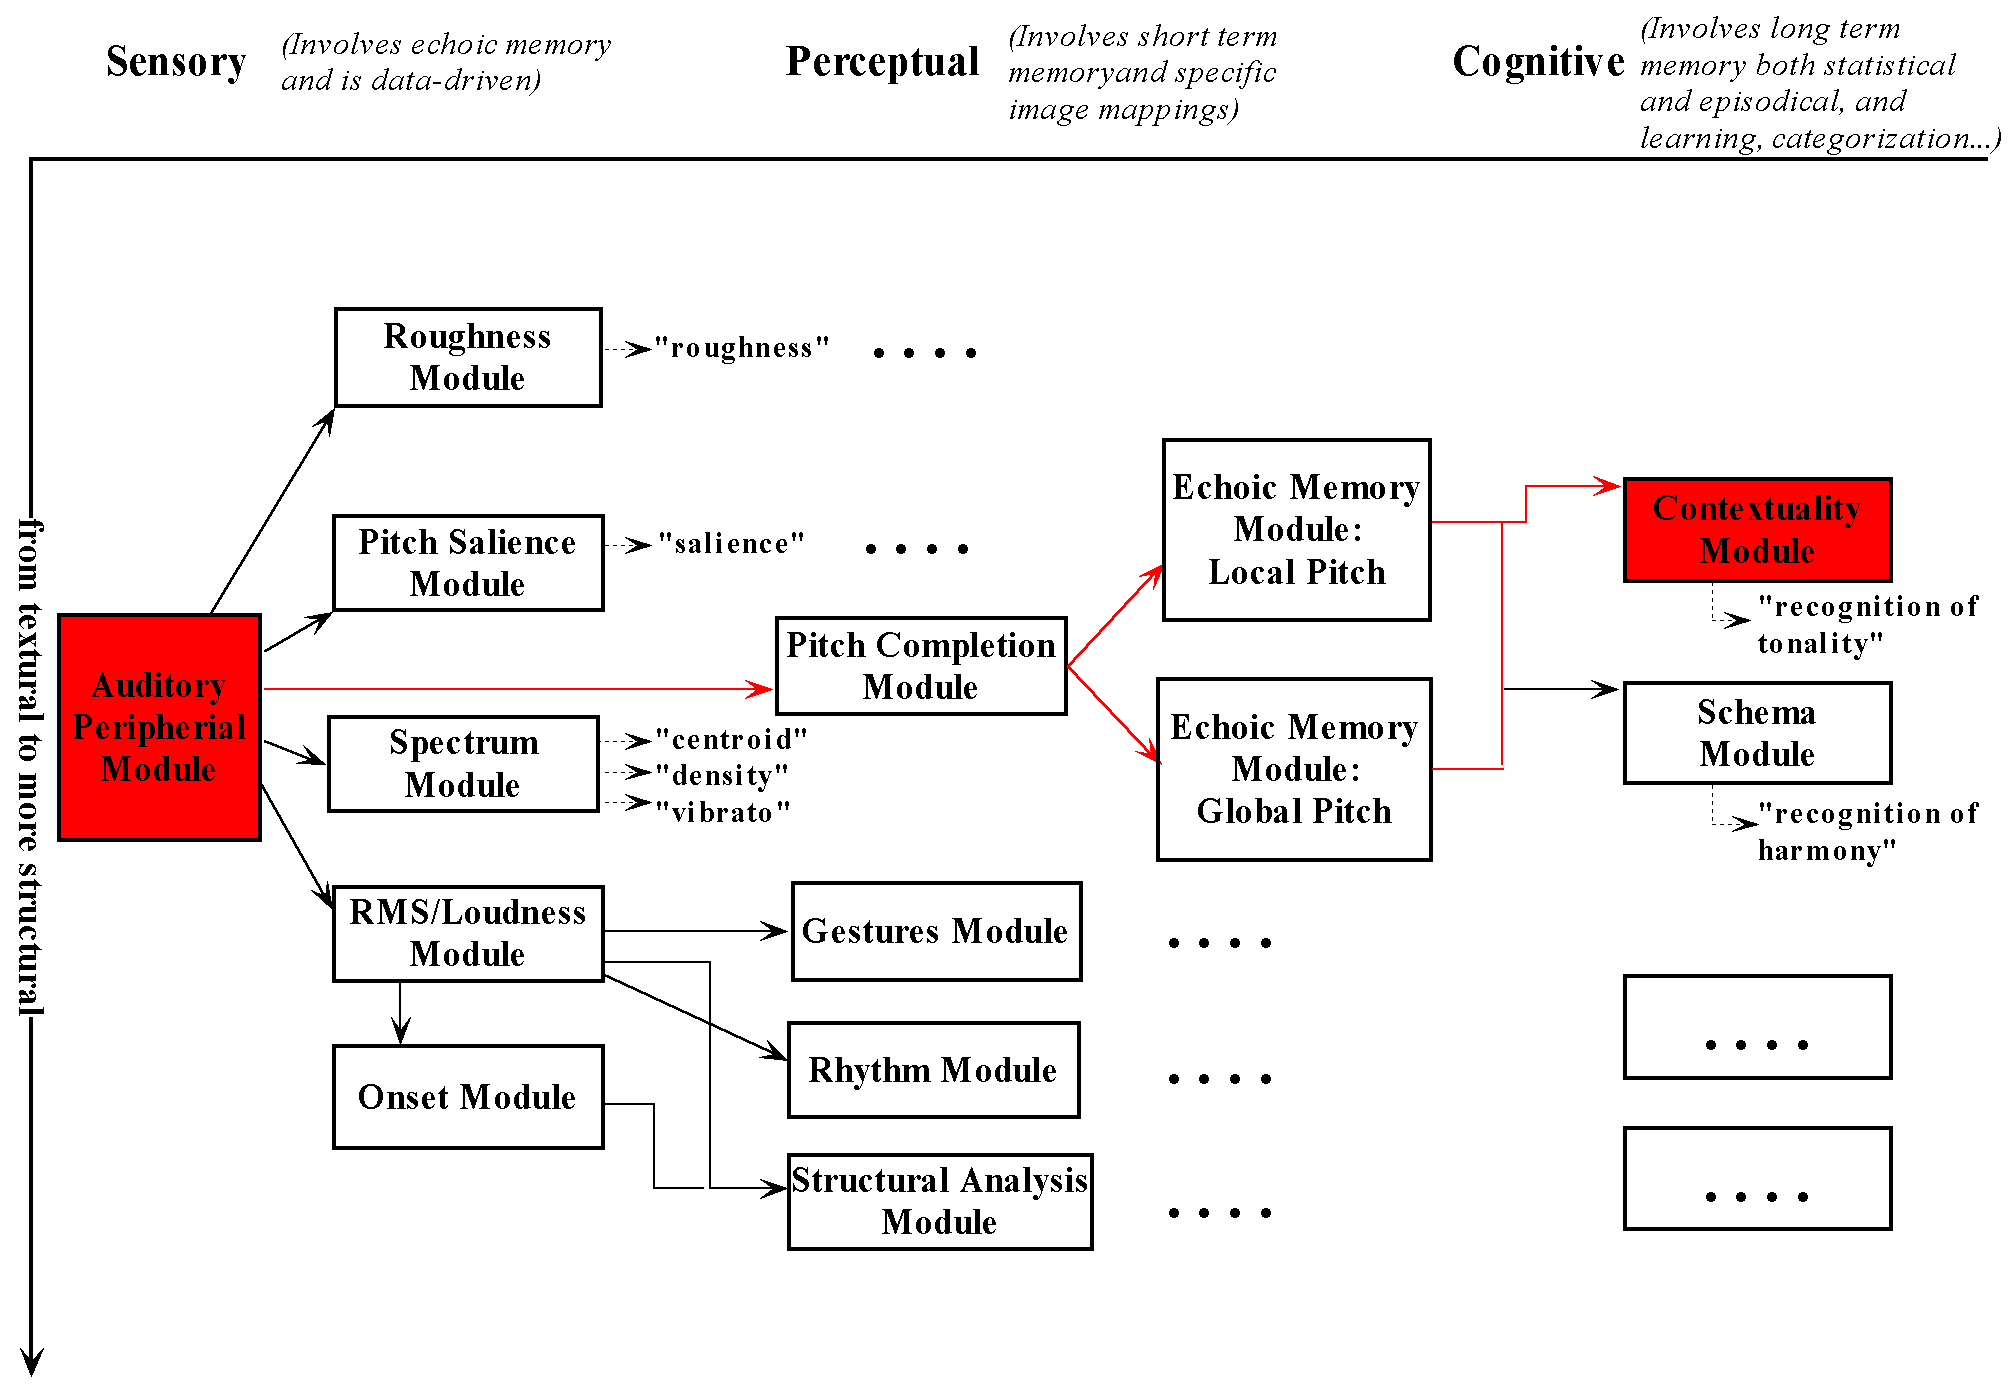
\includegraphics[width=\textwidth]{Graphics/ModulesCM}
    \caption{Chart of image transformation modules, with CM highlighted}
    \label{Fig:ModulesCM}
\end{figure}

Figure \ref{Fig:CMModule} shows the modules involved in the image
transformation and inference process.
\begin{figure}[h]
    \centering
    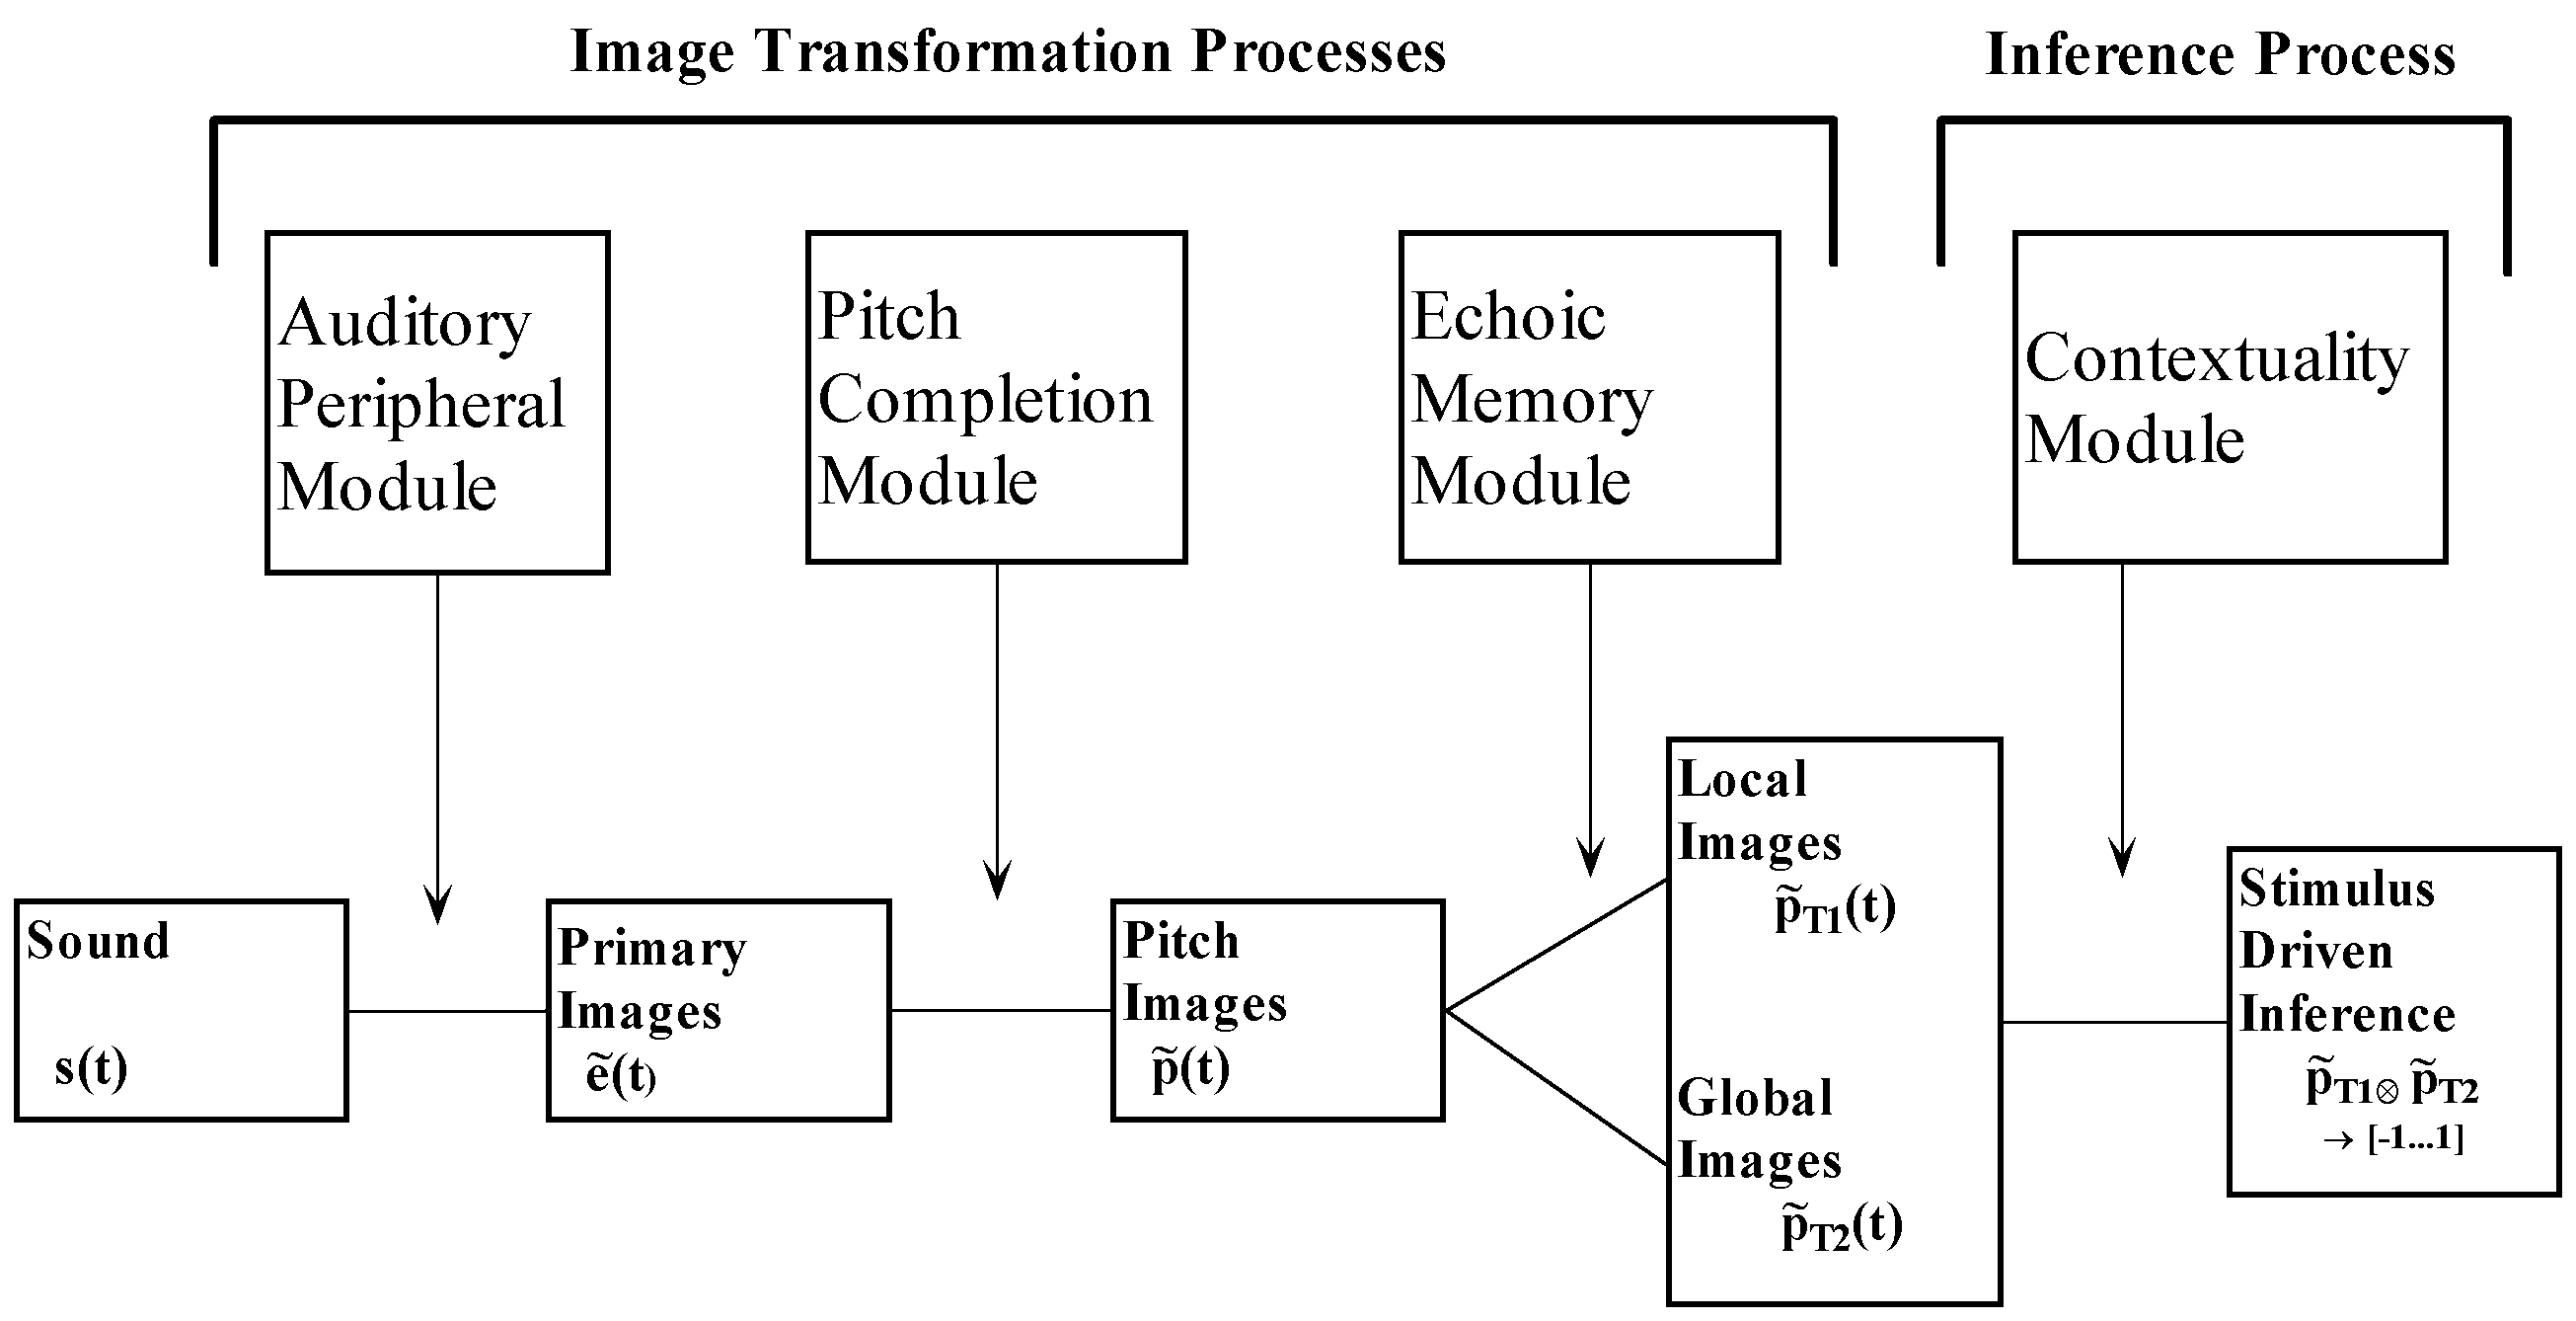
\includegraphics[width=\IPEMDefaultFigureWidth]{Graphics/CMModule}
    \caption{Image Transformation and Inference Process: Contextuality Module}
    \label{Fig:CMModule}
\end{figure}


\subsection{Functional-logical description}
% --------------------------------------------------------------------------------

Contextulatiy realizes a mapping of two images onto a scale:
\begin{equation}
Contextuality: \tilde{p}_{T1} \bigotimes \tilde{p}_{T2} \rightarrow [-1 ... 1]
\end{equation}
where $\tilde{p}$ is a pitch image,
$T1$ and $T2$ are standing for the respective echoes (with T1 $\leq$ T2),
and $\bigotimes$ represents the calculation of a correlation coefficient.
The two methods then correspond to the following mappings:
\begin{itemize}
\item{Inspection:}
    \begin{displaymath}
    Contextuality_{I}: \tilde{p}_{T1}(\tau) \bigotimes \tilde{p}_{T2}(t) \rightarrow [-1 ...
    1]
    \end{displaymath}
    where $\tau$ represents a fixed time instance, typically situated at the end of the
    sound sequence, and $t$ represents the running time.
\item{Comparison:}
    \begin{displaymath}
    Contextulatiy_{II}: \tilde{p}_{T1}(t) \bigotimes \tilde{p}_{T2}(t) \rightarrow [-1 ...
    1]
    \end{displaymath}
    where $t$ represents the running time for both images.
\end{itemize}


\subsection{Signal processing description}
% --------------------------------------------------------------------------------

The Contextuality Module involves several modules.
\begin{itemize}
\item
    The auditory nerve image is calculated using the
    \hyperlink{Concepts:AuditoryPeripheralModule}{Auditory Peripheral
    Module}
\item
    The \hyperlink{Concepts:PitchCompletionModule}{Pitch Completion
    Module} transforms the auditory nerve image into pitch images
\item
    Through the \hyperlink{Concepts:EchoicMemoryModule}{Echoic Memory
    Module} the pitch images undergo the effect of an echo and are
    processed into local and global images
\item
    The Contextuality Module considers two types of contextuality
\end{itemize}


\subsection{Implementation}
% --------------------------------------------------------------------------------

\begin{tabularx}{\linewidth}{llX}
\hyperlink{FuncRef:IPEMContextualityIndex}{IPEMContextualityIndex}
& - & Calculates the contextuality index. Two methods are used:
the method of comparison compares running chords with running tone
center images, while the method of inspection compares a fixed
chord with running chords and running tone center images.
\end{tabularx}


\subsection{Examples}
% --------------------------------------------------------------------------------

Contextuality has been used to simulate the probe-tone experiments
of Krumhansl and Kessler
\cite{article:MusicPerception:Leman:2000,KrumhanslKessler:82}.
%See also \hyperlink{Chapter:ConceptsApplications}{Applications} for more elaborate examples.\\

In what follows, contextuality is applied to the
\IPEMSound{Sounds/SchumannKurioseGeschichte.wav}{short excerpt of
Schumann's Kuriose Geschichte} followed by a 0.1 s period of
silence and an f$\sharp$ Shepard tone. Use the following MATLAB
code to read in the sound file, generate the silence and generate
the Shepard tone f$\sharp$:\\

\begin{IPEMCodeEnvironment}
[s1,fs] = IPEMReadSoundFile('SchumannKurioseGeschichte.wav');
\newline s2 = zeros(1,round(0.1*fs));
\newline NoteFreq = IPEMCalcNoteFrequency('F\#4');
\newline s3 = IPEMShepardTone(NoteFreq,0.5,fs,1,-20);
\end{IPEMCodeEnvironment}\\

Concatenate the 3 sound signals, calculate the auditory nerve
image and from there the periodicity pitch (see also
\hyperlink{Concepts:EchoicMemoryModule}{Echoic Memory Module})
using the following Matlab code:\\

\begin{IPEMCodeEnvironment}
s = [s1 s2 s3];
\newline [ANI,ANIFreq,ANIFilterFreqs] = IPEMCalcANI(s,fs);
\newline [PP,PPFreq,PPPeriods,PPFANI] = IPEMPeriodicityPitch(ANI,ANIFreq,[],[],[],1);
\end{IPEMCodeEnvironment}\\

Then finally, the function
\hyperlink{FuncRef:IPEMContextualityIndex}{IPEMContextualityIndex}
 is applied for the context analysis.\\

\begin{IPEMCodeEnvironment}
[Chords,ToneCenters,LocalInspection,GlobalInspection,LocalGlobalComparison] = ...
\newline IPEMContextualityIndex(PP,PPFreq,PPPeriods,[],0.1,1.5,[],1);
\end{IPEMCodeEnvironment}\\

In this example, \IPEMCodeExtract{PP} contains the periodicity
pitch image of the concatenated sounds, \IPEMCodeExtract{PPFreq}
contains the sampling rate, \IPEMCodeExtract{PPPeriods} contains
the analyzed periods, and the fourth argument specifies the
location of the fixed image. Here, it is left blank, which
defaults to the end of the signal. The local and global echoes are
set to 0.1 s and 1.5 s, respectively, and the plot flag is set to
1.\\

Figure \ref{Fig:ContextualityPitchImages} shows the periodicity
pitch image of the Schumann excerpt followed by the Shepard tone,
the local pitch image, and the global pitch image.\\
The method based on inspection has been applied to the local and
the global pitch images.\\

\IPEMCodeExtract{LocalInspection}
(fig. \ref{Fig:ContextualityLocalInspection}) contains the results
of inspecting the local images with the fixed (local) image. The
graph shows the similarity of the Shepard probe tone of
f$\sharp$ within the Schumann excerpt at a local level.\\

\IPEMCodeExtract{GlobalInspection}
(fig. \ref{Fig:ContextualityGlobalInspection}) contains the
results of inspecting the global images with the fixed (local)
image. The graph shows the similarity of the Shepard probe tone of
f$\sharp$ within the Schumann excerpt at a more global pitch
level.\\

\IPEMCodeExtract{LocalGlobalComparision}
(fig. \ref{Fig:ContextualityLocalGlobalComparison}) contains the
results of comparing the local images with the global images over
the whole piece. It shows the degree in which the local pitch
images (= the level of individual tones and chords) fit with the
global pitch images (= the level of the tone context). At points
where the local image deviates from the global image, such as in a
tonal movement, there will be a low correlation. Inversely, at
points where the local image confirms the global image, there will
be a high correlation.\\

\begin{figure}[h]
    \centering
    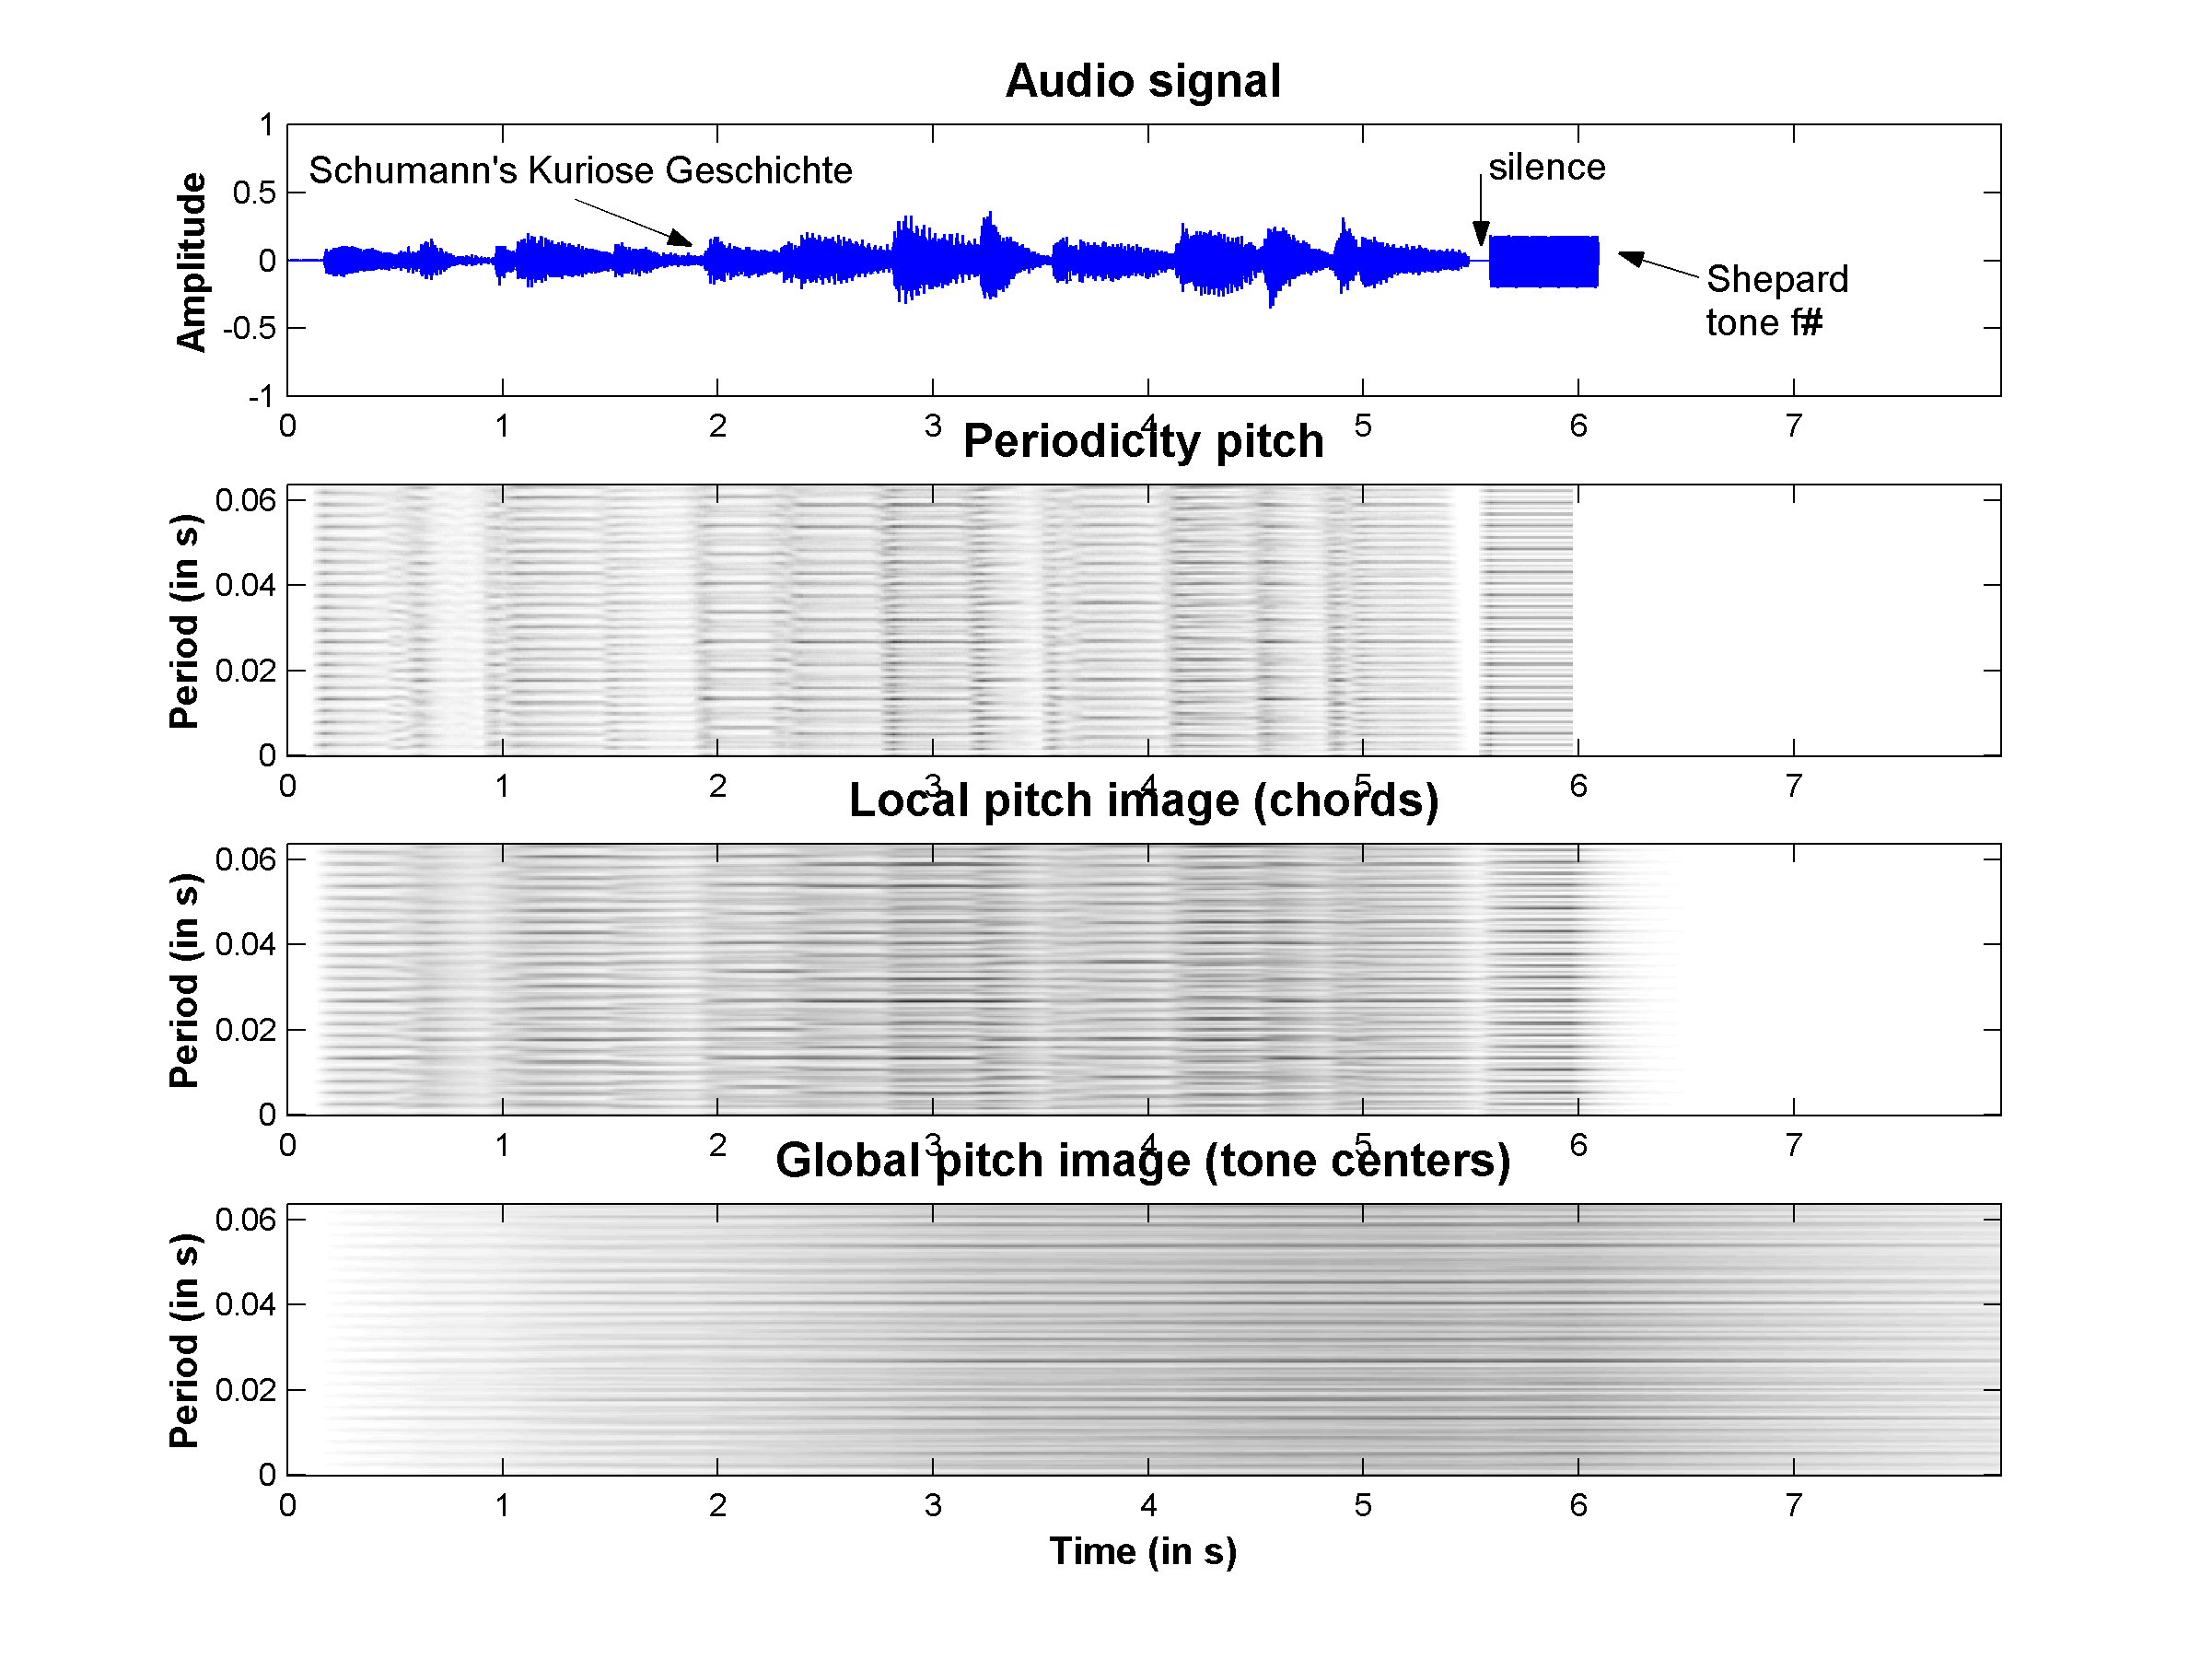
\includegraphics[width=\IPEMDefaultFigureWidth]{Graphics/ContextualityPitchImages}
    \caption{Pitch images for the excerpt of Schumann's Kuriose
    Geschichte followed by a small period of silence and a Shepard
    probe-tone of f$\sharp$. From top to bottom: the analyzed
    audio signal, the periodicity pitch image, the local pitch image and
    the global pitch image.} \label{Fig:ContextualityPitchImages}
\end{figure}

\begin{figure}[h]
    \centering
    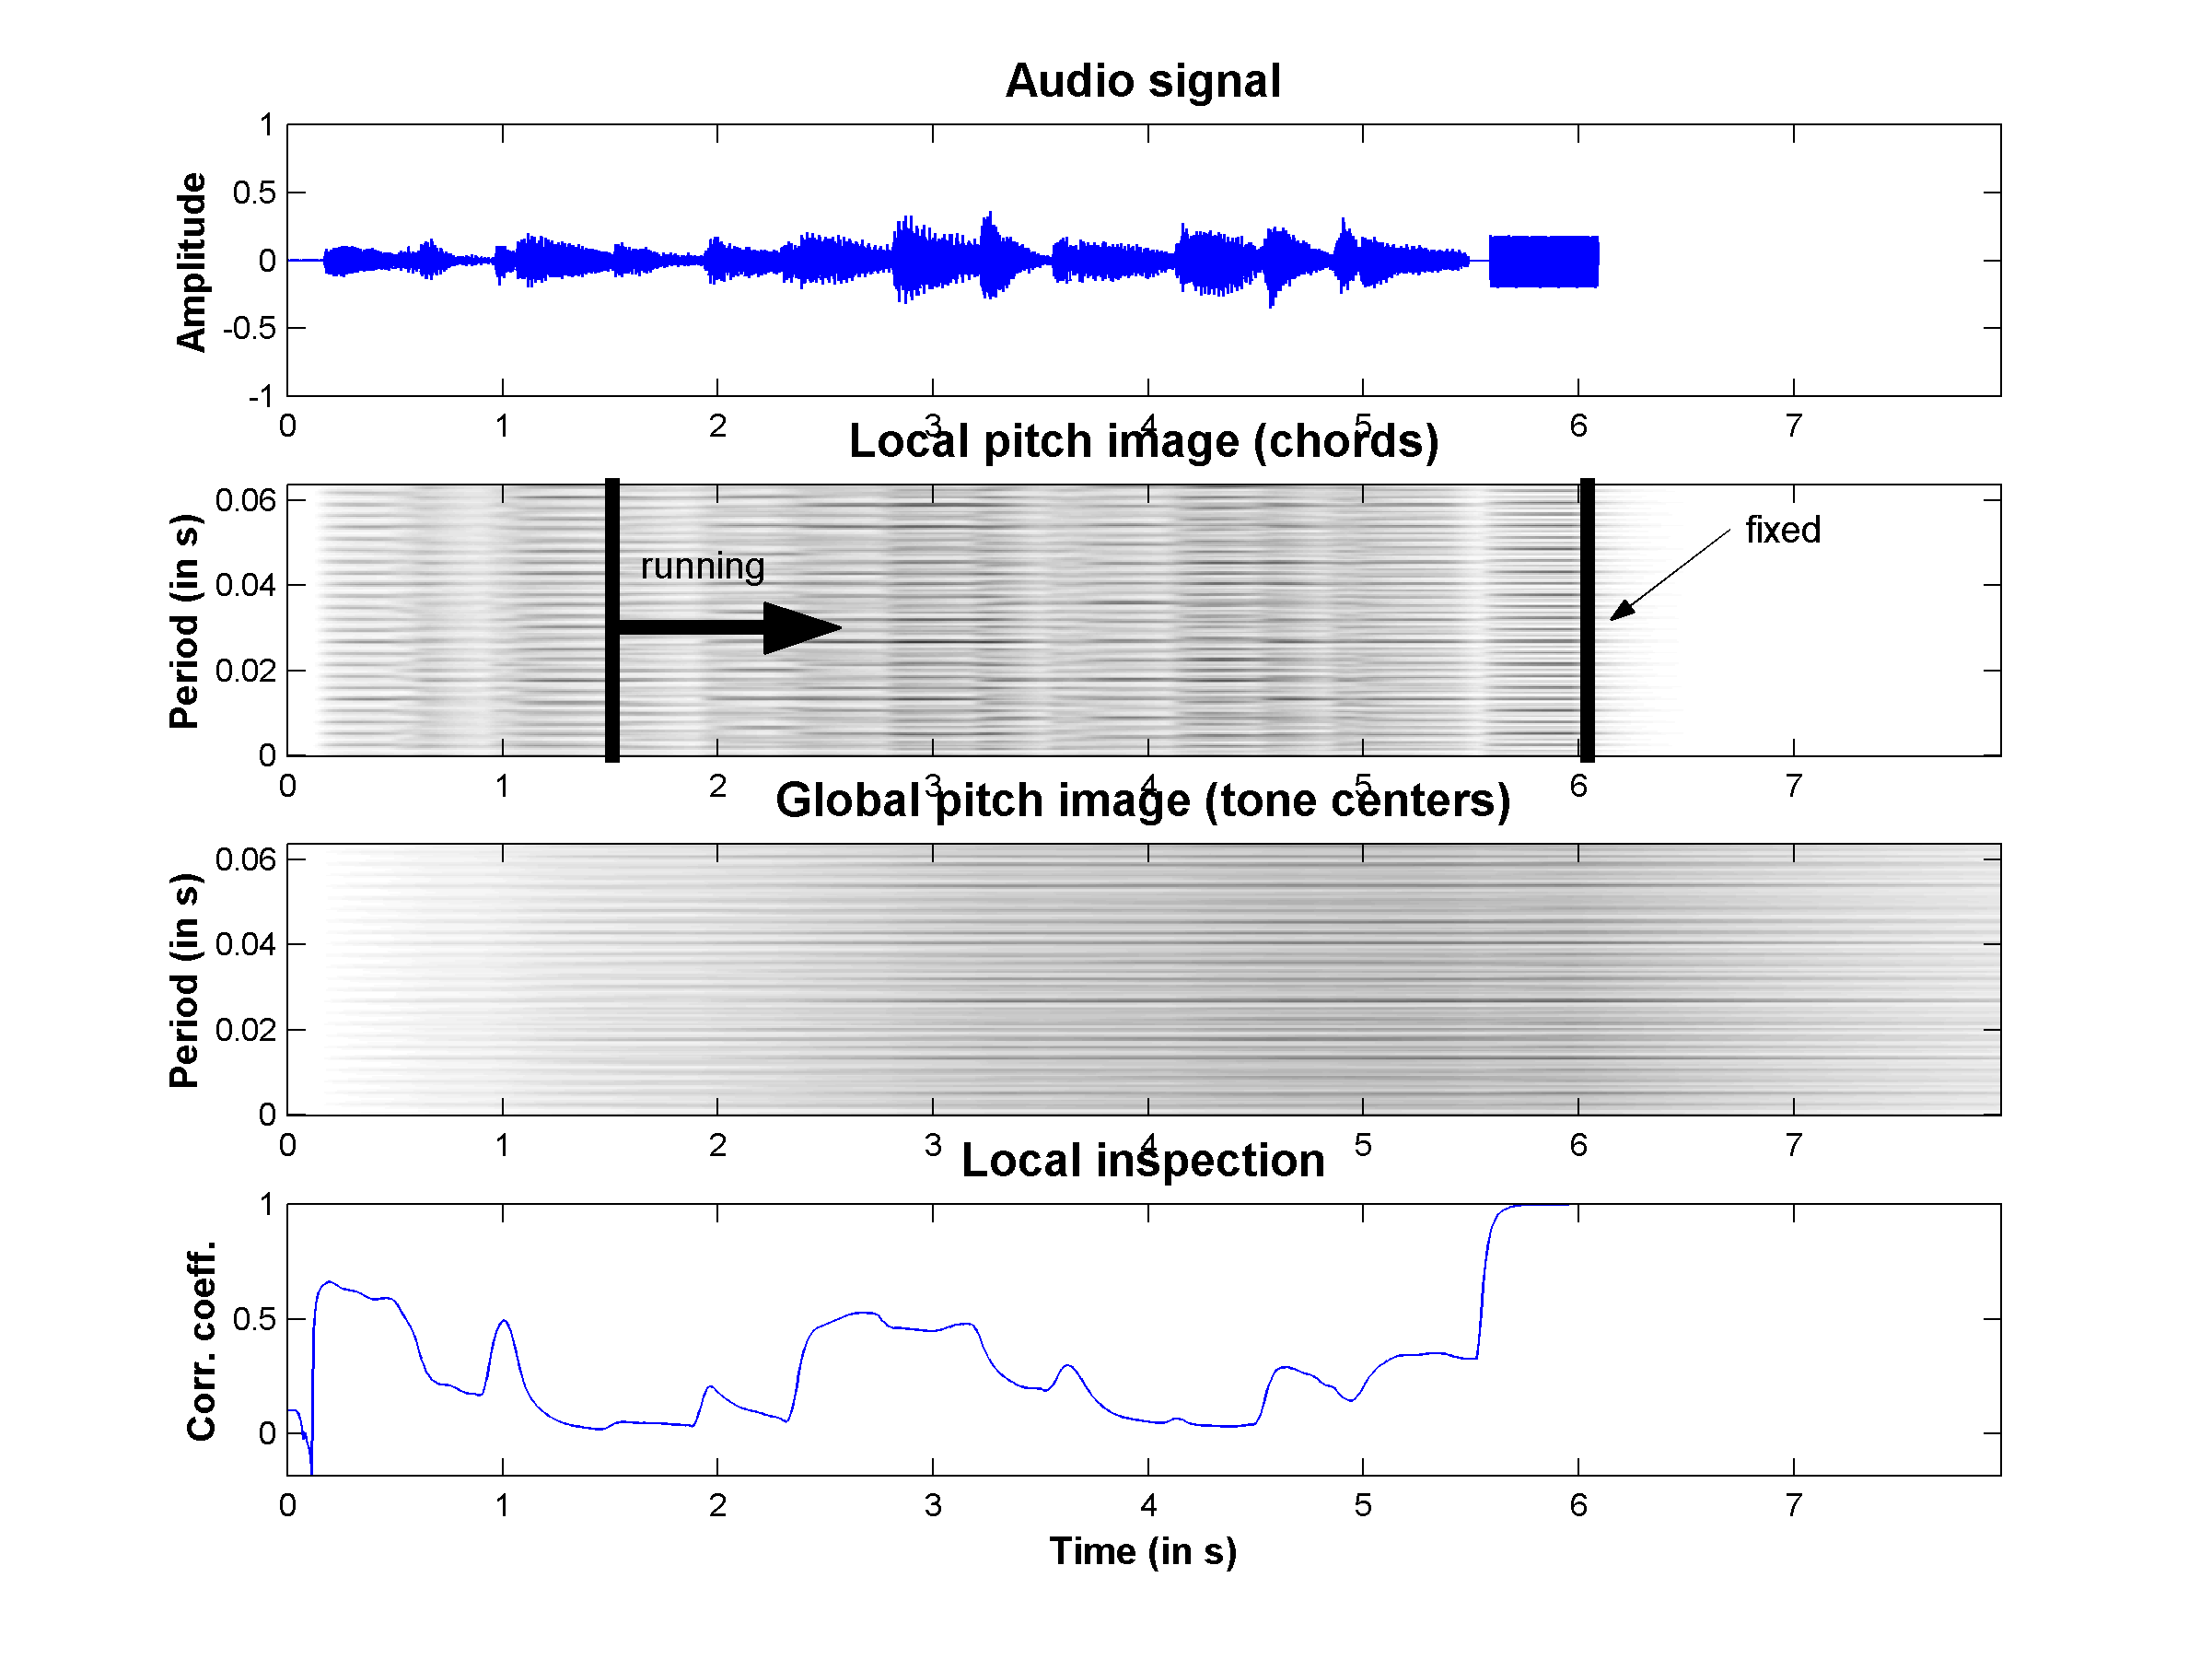
\includegraphics[width=\IPEMDefaultFigureWidth]{Graphics/ContextualityLocalInspection}
    \caption{Inspection of Schumann's Kuriose Geschichte followed
    by a small period of silence and a Shepard probe-tone of
    f$\sharp$. Inspection of local images. From top to bottom:
    audio signal, local pitch image, global pitch image and local
    inspection.} \label{Fig:ContextualityLocalInspection}
\end{figure}

\begin{figure}[h]
    \centering
    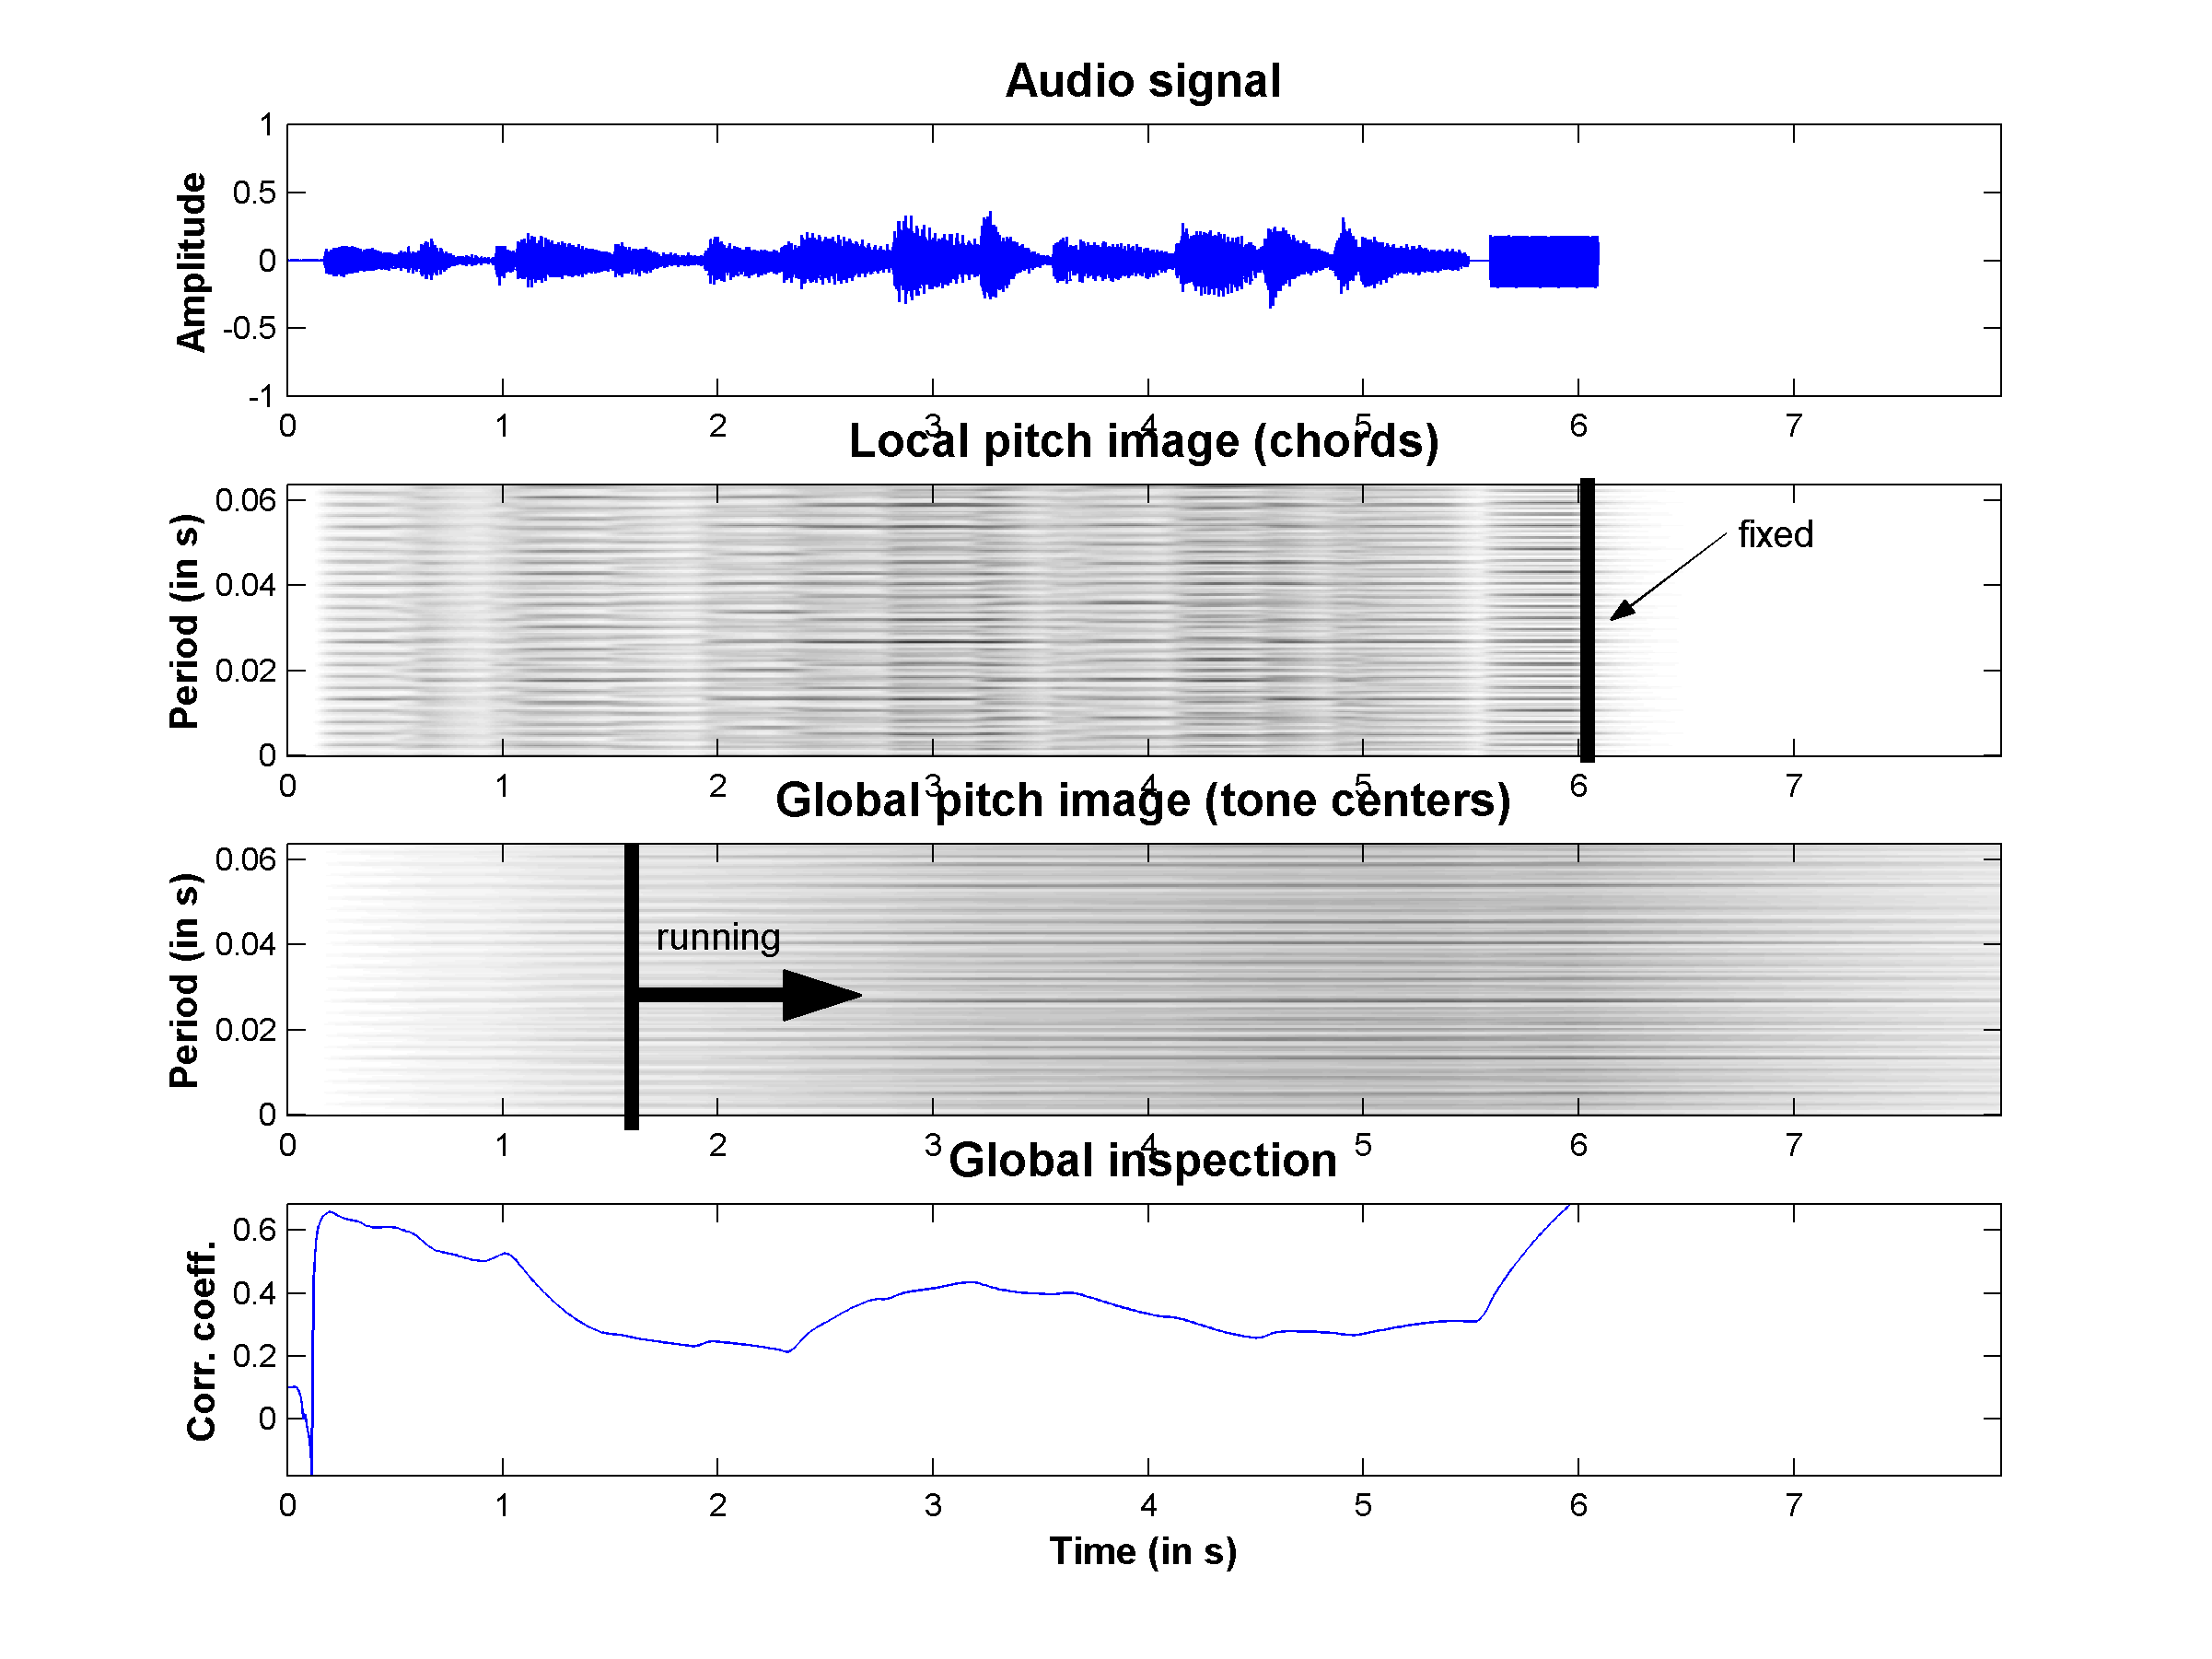
\includegraphics[width=\IPEMDefaultFigureWidth]{Graphics/ContextualityGlobalInspection}
    \caption{Inspection of Schumann's Kuriose Geschichte followed
    by a small period of silence and a Shepard probe-tone of
    f$\sharp$. Inspection of global images. From top to bottom:
    audio signal, local pitch image, global pitch image and global
    inspection} \label{Fig:ContextualityGlobalInspection}
\end{figure}

\begin{figure}[h]
    \centering
    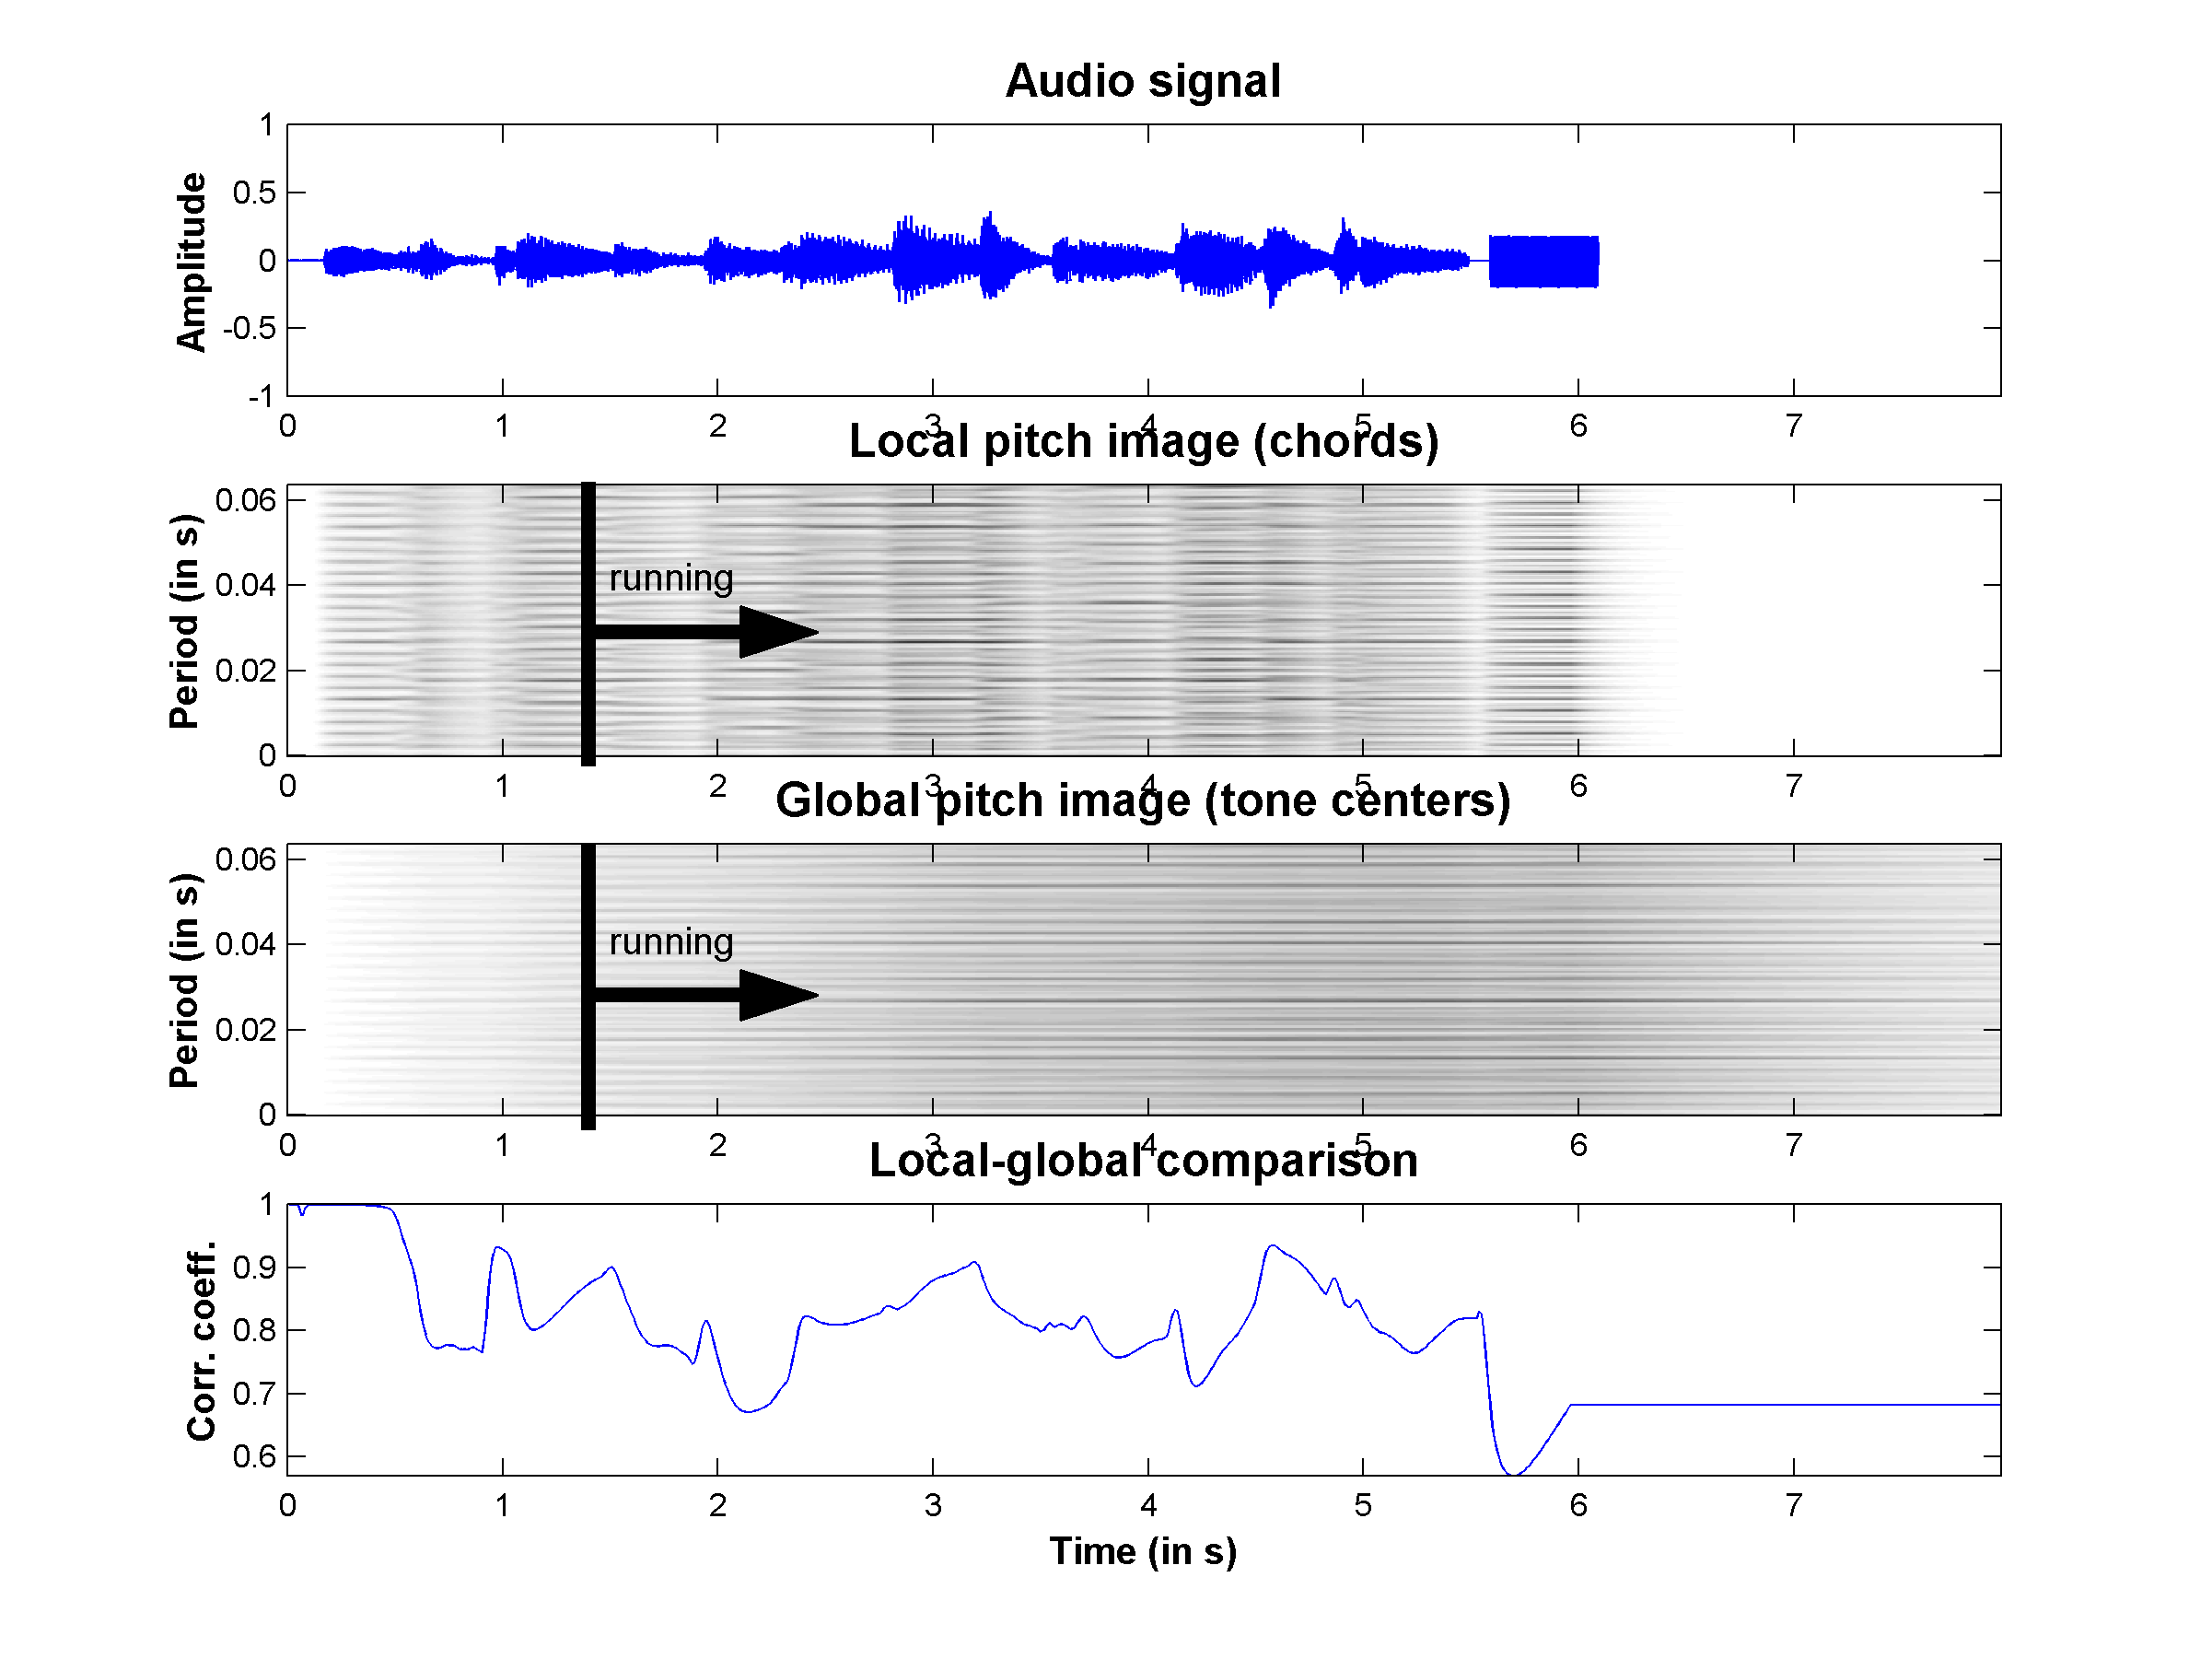
\includegraphics[width=\IPEMDefaultFigureWidth]{Graphics/ContextualityLocalGlobalComparison}
    \caption{Comparison of the local and global pitch images of
    Schumann's Kuriose Geschichte followed by a small period of
    silence and a Shepard probe-tone of f$\sharp$. From top to
    bottom: audio signal, local pitch image, global pitch image
    and comparison between local and global pitch images.}
    \label{Fig:ContextualityLocalGlobalComparison}
\end{figure}

% --------------------------------------------------------------------------------
